\chapter{Fonctions et macros graphiques}\label{cmdFoncGraph}


Ces fonctions et macros créent un élément graphique au moment de leur évaluation et renvoient un résultat égal à \Nil, elles ne sont utilisables \Mytextbf{que lors de la création d'un élément graphique "Utilisateur"}.

Elles peuvent être utilisées dans des macros, mais elles ne seront évaluées que si ces macros sont exécutées lors de la création d'un élément graphique "Utilisateur".


\section{Fonctions graphiques prédéfinies}

<argument>: signifie que l'argument est \Mytextbf{obligatoire}.

[, argument]: signifie que l'argument est \Mytextbf{facultatif}.

Les fonctions prédéfinies sont des fonctions basiques qui ne permettent pas la modification locale des paramètres du graphique, contrairement aux macros graphiques du modèle \textit{draw2d}.

\subsection{(Poly-)Bézier}\label{cmdBezier}
\begin{itemize}
 \item \util \textbf[Bezier()]{Bezier( <liste de points> )}.
 \item \desc dessine une succession de courbes de \textsc{Bézier} (avec éventuellement des segments de droite). Il y a plusieurs possibilités pour la liste de points:
  \begin{enumerate}
  \item une liste de trois points $[A,C,B]$, il s'agit alors d'une courbe de Bézier d'origine \argu{A} et d'extrémité \argu{B} avec un point de contrôle \argu{C}, c'est la courbe paramétrée par: $(1-t)^2A+2t(1-t)C+t^2B$.
  \item une liste de 4 points ou plus: [A1, C1, C2, A2, C3, C4, A3...]: il s'agit alors d'une succession de courbes de Bézier à 2 points de contrôles, la première va de A1 à A2, elle est contrôlée par C1, C2 (paramétrée par $(1-t)^3A1+3(1-t)^2tC1]+3(1-t)t^2C2+t^3A2$), la deuxième va de A2 à A3 et est contrôlée par C3,C4 ...etc. Une exception toutefois, on peut remplacer les deux points de contrôle par la constante \jump, dans ce cas on saute directement de A1 à A2 en traçant un segment de droite.
  \end{enumerate}
\end{itemize}

\begin{demo}{Commande Bezier}{Bezier}
\begin{texgraph}[name=Bezier]
view(-4,4,-4,5),Marges(0,0,0,0),size(7.5),Width:=8,
A:=-3+4*i, B:=3+i, C:=3-3*i, D:=-3-3*i,
C1:=4.5*i,C2:=-2*i, C3:=2-i, C4:=-2,
FillStyle:=full, FillColor:=lightblue,Color:=red,
Bezier([A,C1,C2,B,jump,C,C3,C4,D,jump,A]),
FillStyle:=none, Color:=black, DotStyle:=cross, DotScale:=2,
L:=[A,"$A$","N",B,"$B$","E",C,"$C$","SE",D,"$D$","SO",
C1,"$C_1$","E",C2,"$C_2$","SO",C3,"$C_3$","N",
C4,"$C_4$","N"],
for Z in L By 3 do
 draw("label",Z[2],[anchor:=Z[1],labeldir:=Z[3],showdot:=1])
od,
LineStyle:=userdash, DashPattern:=[5,2,0.5,2],Width:=6,
Line([A,C1,C2,B,jump,C,C3,C4,D])
\end{texgraph}
\end{demo}

\subsection{Cartesian}\label{cmdCartesienne}
\begin{itemize}
 \item \util \textbf[Cartesian()]{Cartesian( <f(x)> [, n, 1] )} ou \textbf[Cartesienne()]{Cartesienne( <f(x)> [, n, 1] )}.
 \item \desc trace la courbe cartésienne d'équation $y=f(x)$. Le paramètre optionnel \argu{n} est un entier (égal à 5 par défaut) qui permet de faire varier le pas de la manière suivante: lorsque la distance entre deux points consécutifs est supérieur à un certain seuil alors on calcule un point intermédiaire [par dichotomie], ceci peut être répété n fois. Si au bout de n itérations la distance entre deux points consécutifs est toujours supérieure au seuil, et si la valeur optionnelle $1$ est présente, alors une discontinuité (\jump) est insérée dans la liste des points.
\end{itemize}

\begin{demo}{Courbe avec discontinuités}{Cartesienne}
\begin{texgraph}[name=Cartesienne]
view(-2,2,-0.1,2),Marges(0.5,0.5,0.5,0.5),size(7.5),
tMin:=-2, tMax:=2, Width:=8,
draw("grid",[-2,2+2*i],[unit:=[0.5,0.5],gridstyle:=dotted]),
Axes(0,1+i,1), NbPoints:=100, Color:=darkseagreen,
Cartesian(x*Ent(1/x),5,1)
\end{texgraph}
\end{demo}

\subsection{Dot (nuage de points)}\label{cmdPoint}
\begin{itemize}
 \item \util \textbf[Dot()]{Dot( <A1>, ..., <An> )} ou \textbf[Point()]{Point( <A1>, ..., <An> )}.
 \item \desc représente le nuage de points \argu{A1} ... \argu{An}.
\end{itemize}

\pngtrue
\begin{demo}{Diagramme de bifurcation de la suite $u_{n+1}=ru_n(1-u_n)$}{Point}
\begin{texgraph}[name=Point,export=none]
view(2.75,4,0,1),
Marges(0.75,0.5,0.5,0.5),size(7.5),
Axes(Xmin+i*Ymin,0.25+0.2*i,1+i),
pas:=0.001, Color:=red,
DotScale:=0.1,
Dot(
 for r from Xmin to Xmax step pas do
 u:=0.5,
 for k from 1 to 25 do u:=r*u*(1-u) od,
 for k from 1 to 25 do u:=r*u*(1-u), r+i*u od
 od)
\end{texgraph}
\end{demo}
\pngfalse

\subsection{Ellipse}\label{cmdEllipse}
\begin{itemize}
 \item \util \textbf[Ellipse()]{Ellipse( <A>, <Rx>, <Ry> [, inclinaison] )}.
 \item \desc trace une ellipse de centre \argu{A} de rayons \argu{Rx} et \argu{Ry} sur les axes respectifs $Ox$ et $Oy$. Le dernier paramètre \argu{inclinaison} est un angle en degrés (nul par défaut) qui indique l'inclinaison de l'ellipse par rapport à l'horizontale.
\end{itemize}

\begin{demo}{Ellipses}{ellipse}
\begin{texgraph}[name=ellipse]
view(-5.25,5.25,-5.25,5.25), Marges(0,0,0,0), size(7.5),
background(full,blue), Width:=4, Color:=white,
inclin:=[0,35,-35],
for z in inclin do
 Ellipse(0,5,2,z)
od,
Width:=2*mm, Ellipse(0,1.5,4.5),
Label(-0.1, "\resizebox{6cm}{3.5cm}{R\ T\ F}")
\end{texgraph}
\end{demo}

\subsection{EllipticArc}\label{cmdEllipticArc}
\begin{itemize}
 \item \util \textbf[EllipticArc()]{EllipticArc( <B>, <A>, <C>, <Rx>, <Ry> [, sens] )}.
 \item \desc trace un arc d'ellipse dont les axes sont $Ox$ et $Oy$ et le centre \argu{A},  le rayon sur $Ox$ est \argu{Rx}, et celui sur $Oy$ est \argu{Ry}. L'arc est tracé partant de la droite $(AB)$ jusqu'à la droite $(AC)$, l'argument facultatif \argu{sens} indique: le sens trigonométrique si sa valeur est $1$ (valeur par défaut), le sens contraire si sa valeur est $-1$. 
\end{itemize}

\begin{demo}{Commande EllipticArc}{EllipticArc}
\begin{texgraph}[name=EllipticArc]
view(-2.25,3.75,-2,5),Marges(0,0,0,0),size(7.5),
A:=0, B:=3+i, C:=2+4*i, DotScale:=2, Width:=8,
Ligne([B,A,C],0), Color:=red,
LabelDot(A,"$A$","S",1), LabelDot(B,"$B$","N",1),
LabelDot(C,"$C$","SE",1), Arrows:=1, Color:=blue,
EllipticArc(B,A,C,2,1,-1), EllipticArc(B,A,C,2,3,1)
\end{texgraph}
\end{demo}

Remarques: 
\begin{itemize}
 \item Pour un arc de cercle, il suffit de prendre \argu{Rx} et \argu{Ry} égaux. Mais le plus simple est d'utiliser la macro \Helpref{Arc}{macArc}.
 \item Pour un arc d'ellipse dont l'axe portant le rayon \argu{Rx} a une inclinaison non nulle par rapport à l'axe horizontal, il faut utiliser la commande \co{draw("ellipticArc",...)}, ou bien la macro \Helpref{ellipticArc}{macellipticArc}.
\end{itemize}

\subsection{Implicit}\label{cmdImplicit}
\begin{itemize}
 \item \util \textbf[Implicit()]{Implicit( <f(x,y)> [, n, m] )}.
 \item \desc trace la courbe implicite d'équation $f(x,y)=0$. L'intervalle des abscisses est subdivisé en \argu{n} parties et l'intervalle des ordonnées en \argu{m} parties, par défaut $n=m=50$. Sur chaque pavé ainsi obtenu on teste s'il y a un changement de signe, auquel cas on applique une dichotomie sur les bords du pavé.
\end{itemize}

\begin{demo}{\'Equation $\sin(xy)=0$}{Implicit}
\begin{texgraph}[name=Implicit]
view(-5,5,-5,5),Marges(0,0,0,0), size(7.5), 
Arrows:=1, Axes(0,1+i), Arrows:=0,
Width:=8, Color:=red,
Implicit( sin(x*y) )
\end{texgraph}
\end{demo}

\subsection{Label}\label{cmdLabel}
\begin{itemize}
 \item \util \textbf[Label()]{Label( <affixe1>, <texte1>,..., <affixeN>, <texteN> )}.
 \item \desc place la chaîne de caractères \argu{texte1} à la position \argu{affixe1} ... etc. Les paramètres \argu{texte1},..., \argu{texteN} sont donc interprétés comme des \Helpref{chaînes de caractères}{chaine}.
\end{itemize}

\begin{demo}{Nommer des points}{Label}
\begin{texgraph}[name=Label,
       preload="PolyedresII.mac"]
view(-5,5,-5,5),Marges(0,0,0,0), size(7.5,0),
C:=Cube(Origin, M(3,3,0)), S:=Sommets(C), 
Point3D(S), DrawPoly(C,0), k:=0,
for Z in S by 2 do
 Inc(k,1),
 Label(Proj3D(Z)+if k>4 then 0.5*i else -0.5*i fi,
   ["$S_",k,"$"])
od 
\end{texgraph}
\end{demo}

\subsection{Line (Ligne polygonale)}\label{cmdLigne}
\begin{itemize}
 \item \util \textbf[Line()]{Line( <list>, <closed> [, radius] )} ou \textbf[Ligne()]{Ligne( <liste>, <fermée> [, rayon] )}.
 \item \desc trace la ligne polygonale définie par la liste, si le paramètre \argu{fermée} vaut 1, la ligne polygonale sera fermée, si sa valeur est 0 la ligne est ouverte. Si l'argument \argu{rayon} est précisé (0 par défaut), alors les "angles" de la ligne polygonale sont arrondis avec un arc de cercle dont le rayon correspond à l'argument \argu{rayon}.
\end{itemize}

\begin{demo}{Triangle de \textsc{Sierpinski}}{Ligne}
\begin{texgraph}[name=Ligne]
Marges(0,0,0,0), size(7.5),
A:=-5-5*i, B:=5*i, C:=5-5*i, niv:=6,
Tr:=[A,B,C,jump], {figure initiale}
for k from 1 to niv do
 Tr:=[hom(Tr,A,0.5),hom(Tr,B,0.5),hom(Tr,C,0.5)]
od,
FillStyle:=full, FillColor:=blue, Line(Tr,1) 
\end{texgraph}
\end{demo}

\subsection{Odeint (ou EquaDif)}\label{cmdEquadif}
\begin{itemize}
 \item \util \textbf[EquaDif()]{Odeint( <f(t,x,y)>, <t0>, <x0 + i*y0> [, mode] )}.
 \item \desc trace une solution approchée de l'équation différentielle: $x'(t)+iy'(t)=f(t,x,y)$ avec la condition initiale $x(t_0)=x0$ et $y(t_0)=y_0$. Le dernier paramètre est facultatif et peut valoir 0, 1 ou 2:
  \begin{itemize}
  \item \argu{mode}=0: la courbe représente les points de coordonnées $(x(t),y(t))$, c'est la valeur par défaut.
  \item \argu{mode}=1: la courbe représente les points de coordonnées $(t,x(t))$.
  \item \argu{mode}=2: la courbe représente les points de coordonnées $(t,y(t))$.
  \end{itemize}
C'est la méthode de \textsc{Runge-Kutta} d'ordre 4 qui est utilisée.
 \item \exem l'équation $x''-x'-tx=\sin(t)$ avec la condition initiale $x(0)=-1$ et $x'(0)=1/2$, se met sous la forme:
\[\begin{pmatrix}
X'\\Y'\end{pmatrix}=\begin{pmatrix} 0&1\\t&1\end{pmatrix}\begin{pmatrix}X\\Y\end{pmatrix}+
\begin{pmatrix}0\\\sin(t)\end{pmatrix}\] en posant $X=x$ et $Y=x'$:
\end{itemize}

\begin{demo}{\'Equation différentielle}{EquaDif}
\begin{texgraph}[name=EquaDif]
view(-10.5,2.5,-1.5,4.5),Marges(0,0,0,0), size(7.5,0),
draw("axes",[0,2+i],[legend:=["$x$","$t$"],Arrows:=1,
 nbsubdiv:=[1,0]]),
Width:=8, Color:=red, tMin:=-10, tMax:=2,
Odeint(y+i*(t*x+y+sin(t)),0,-1+i/2, 1),
Color:=black, LabelStyle:=stacked,
Label(-6+2*i,
 "$x''-x'-tx=\sin(t)$\\avec $x(0)=-1$ et $x'(0)=\frac12$")
\end{texgraph}
\end{demo}


\subsection{Parametric (ou Courbe)}\label{cmdCourbe}
\begin{itemize}
 \item \util \textbf[Parametric()]{Parametric( <f(t)> [, n, 1] )} ou \textbf[Courbe()]{Courbe( <f(t)> [, n, 1] )}.
 \item \desc trace la courbe paramétrée par \argu{f(t)} où $f$ est à valeurs complexes.

Le paramètre optionnel \argu{n} est un entier (égal à 5 par défaut) qui permet de faire varier le pas de la manière suivante : lorsque la distance entre deux points consécutifs est supérieur à un certain seuil alors on calcule un point intermédiaire (par dichotomie), ceci peut être répété $n$ fois. Si au bout de $n$ itérations la distance entre deux points consécutifs est toujours supérieure au seuil, et si la valeur optionnelle $1$ est présente, alors une discontinuité (\jump) est insérée dans la liste des points.
\end{itemize}

\subsection{Path}\label{cmdPath}
\begin{itemize}
 \item \util  \textbf[Path()]{Path( <liste> [, fermé (0/1)]}
 \item \desc trace le chemin représenté par \argu{liste} et ferme la dernière composante de celui-ci si l'argument optionnel vaut $1$ (sa valeur par défaut est $0$). La liste est une succession de points (affixes) et d'instructions indiquant à quoi correspondent ces points, ces instructions sont: 
\begin{itemize}
 \item \Mytextbf{line}: relie les points par une ligne polygonale,
 \item \Mytextbf{linearc}: relie les points par une ligne polygonale mais les angles sont arrondis par un arc de cercle, la valeur précédent la commande linearc est interprétée comme le rayon de ces arcs.
 \item \Mytextbf{clinearc}: même effet que \emph{linearc}, sauf que la ligne polygonale est refermée avant d'arrondir les angles.
 \item \Mytextbf{arc}: dessine un arc de cercle, ce qui nécessite quatre arguments: 3 points (départ, centre, arrivée) et le rayon, plus éventuellement un cinquième argument: le sens (+/- 1), le sens par défaut est 1 (sens trigonométrique).
 \item \Mytextbf{ellipticArc}: dessine un arc d'ellipse, ce qui nécessite cinq arguments: 3 points, le rayonX, le rayonY, plus éventuellement un sixième argument: le sens (+/- 1), le sens par défaut est 1 (sens trigonométrique), plus éventuellement un septième argument: l'inclinaison en degrés du grand axe par rapport à l'horizontale.
 \item \Mytextbf{curve}: relie les points par une spline cubique naturelle.
 \item \Mytextbf{bezier}: relie le premier et le quatrième point par une courbe de Bézier (les deuxième et troisième points sont les points de contrôle).
 \item \Mytextbf{circle}: dessine un cercle, ce qui nécessite deux arguments: un point et le centre, ou bien trois arguments qui sont trois points du cercle.
 \item \Mytextbf{ellipse}: dessine une ellipse, les arguments sont: un point, le centre, rayon rX, rayon rY, inclinaison du grand axe en degrés par rapport à l'horizontale (facultatif).
 \item \Mytextbf{move}: indique un déplacement sans tracé.
 \item \Mytextbf{closepath}: ferme la composante en cours.
\end{itemize}
Par convention, le premier point du tronçon numéro n+1 est le dernier point du tronçon numéro n.
 \item \exem
\end{itemize}

\begin{demo}{Commande Path et Eofill}{Path}
\begin{texgraph}[name=Path]
view(-5,5,-4,6), Marges(0,0,0,0), size(7.5),
Axes(2*i,1+i), 
Eofill:=1, FillStyle:=full, FillOpacity:=0.85,
FillColor:= blue, Width:=8,
Path([-4,i,circle,
   -3+2*i,move,-3,-2,line,
   0,2,2,-1,arc,
   3,3+3*i,0.5,linearc,
   1,-1+5*i,-3+2*i,bezier,
   closepath,
   ]) 
\end{texgraph}
\end{demo}

\subsection{Polar (ou Polaire)}\label{cmdPolaire}
\begin{itemize}
 \item \util \textbf[Polar()]{Polar( <r(t)> [, n, 0/1] )} ou \textbf[Polaire()]{Polaire( <r(t)> [, n, 0/1] )}.
 \item \desc trace la courbe polaire d'équation $\rho=r(t)$, \argu{expression}. Le paramètre optionnel \argu{n} est un entier (égal à 5 par défaut) qui permet de faire varier le pas de la manière suivante: lorsque la distance entre deux points consécutifs est supérieur à un certain seuil alors on calcule un point intermédiaire (par dichotomie), ceci peut être répété $n$ fois. Si au bout de $n$ itérations la distance entre deux points consécutifs est toujours supérieure au seuil, et si la valeur optionnelle $1$ est présente, alors une discontinuité (\jump) est insérée dans la liste des points.
\end{itemize}

\begin{demo}{Courbe polaire et points doubles}{Polaire}
\begin{texgraph}[name=Polaire]
view(-3,2,-2,3),Marges(0.25,0.25,0.25,0.25), size(7.5),
Axes(0,1+i), NbPoints:=250, tMin:=-25, tMax:=25,
courbe:=Get(Polar((t+1)/(t-1))),
ptDoubles:= courbe InterL courbe,
Width:=8, Color:= blue, Line(courbe),
DotStyle:=dotcircle, DotScale:=1.5, Dot(ptDoubles),
Label(1+2*i,"$r(t)=\dfrac{t+1}{t-1}$")
\end{texgraph}
\end{demo}

\subsection{Spline}\label{cmdSpline}
\begin{itemize}
 \item \util \textbf[Spline()]{Spline( <V0>, <A0>,..., <An>, <Vn> )}.
 \item \desc trace la spline cubique passant par les points \argu{A0} jusqu'à \argu{An}. \argu{V0} et \argu{Vn} désignent les vecteurs vitesses aux extrémités [contraintes], si l'un d'eux est nul alors l'extrémité correspondante est considérée comme libre (sans contrainte).
\end{itemize}

\begin{demo}{Commande Spline}{Spline}
\begin{texgraph}[name=Spline]
view(-5,5,-5,5), Marges(0.25,0.25,0.25,0.25), size(7.5),
Axes(0,1+i),
A:= -4-3*i, B:=-2+2*i, C:=1-3*i, D:=4+3*i,
LabelDot(A,"$A$","S",1), LabelDot(B,"$B$","N",1),
LabelDot(C,"$C$","S",1), LabelDot(D,"$D$","O",1),
Width:=8, Color:=red, Spline(0,A,B,C,D,0),
Line([-4.5+4.5*i,-4+4.5*i]), LabelStyle:=left,
Label(-3.5+4.5*i,"libre"), Color:=blue, Spline(5,A,B,C,D,5*i),
Line([-4.5+3.5*i,-4+3.5*i]), Label(-3.5+3.5*i,"contrainte"),
Width:=4, Arrows:=1, Line([A,A+2,jump,D,D+2*i])
\end{texgraph}
\end{demo}

\subsection{StraightL (droite)}\label{cmdDroite}
\begin{itemize}
 \item \util \textbf[StraightL()]{StraightL( <A>, <B> [, C] )} ou \textbf[Droite()]{Droite( <A>, <B> [, C] )} .
 \item \desc trace la droite $(AB)$ lorsque le troisième argument \argu{C} est omis, sinon c'est la droite d'équation cartésienne \argu{A}x+\argu{B}y=\argu{C}.
\end{itemize}

\begin{demo}{Développée d'une ellipse}{Droite}
\begin{texgraph}[name=Droite]
view(-5,5,-5,5), Marges(0,0,0,0), size(7.5),
F:=sqrt(7), F':=-F, {foyers} Width:=1, Color:=darkgray,
for t from -pi to pi step 0.1 do
 M:=4*cos(t)+3*i*sin(t),
 Vn:=(M-F)/abs(M-F)+(M-F')/abs(M-F'),
 StraightL(M,M+Vn), {normale a l'ellipse}
od,
Width:=8, Color:=red, Ellipse(0,4,3),
LabelDot(F,"$F$","S",1), LabelDot(F',"$F'$","S",1)
\end{texgraph}
\end{demo}


\section{Commandes de dessin bitmap}

La version \version propose quelques commandes de base pour faire du dessin bitmap. Ce dessin bitmap peut être enregistré (au format \textit{bmp}) mais il n'est pas pris en compte par les autres exports du logiciel. Ces commandes ne sont fonctionnelles qu'avec la version GUI de TeXgraph. Chaque pixel est repéré son affixe $x+iy$ où $x$ et $y$ sont deux entiers, l'origine est en haut à gauche de la zone de dessin \Mytextbf{marges exclues}, l'axe $Ox$ est dirigé vers la droite et l'axe $Oy$ vers le bas.

\subsection{DelBitmap}\label{cmdDelBitmap}
\begin{itemize}
 \item \util \textbf[DelBitmap()]{DelBitmap()}.
 \item \desc détruit le bitmap en cours.
\end{itemize}

\subsection{GetPixel}\label{cmdGetPixel}
\begin{itemize}
 \item \util \textbf[GetPixel()]{GetPixel( <liste d'affixes de pixels> )}.
 \item \desc renvoie la liste des couleurs des pixels de la \argu{liste} de pixels. Les affixes des pixels sont de la forme $a+ib$ avec $a$ et $b$ des entiers positifs ou nuls, l'origine étant le coin supérieur gauche de la zone graphique \Mytextbf{marges exclues}.
\end{itemize}

\subsection{MaxPixels}\label{cmdMaxPixels}
\begin{itemize}
 \item \util \textbf[MaxPixels()]{MaxPixels()}.
 \item \desc renvoie la taille de la zone graphique en pixels sous la forme: \textsl{maxX+i*maxY}, ainsi pour les coordonnées des pixels (coordonnées entières), l'intervalle des abscisses est \textsl{[0 .. maxX]} et celui des ordonnées \textsl{[0 .. maxY]}. Chaque pixel est repéré par des coordonnées entières, donc chaque pixel a une affixe $a+ib$ avec $a$ dans \textsl{[0 .. maxX]} et $b$ dans \textsl{[0 .. maxY]}. L'origine étant le coin supérieur gauche de la zone graphique \Mytextbf{marges exclues}.
\end{itemize}

\subsection{NewBitmap}\label{cmdNewBitmap}
\begin{itemize}
 \item \util \textbf[NewBitmap()]{NewBitmap( [fond] )}.
 \item \desc permet de créer un nouveau bitmap (vide). Par défaut la couleur du fond est le blanc.
\end{itemize}

\subsection{Pixel}\label{cmdPixel}
\begin{itemize}
 \item \util \textbf[Pixel()]{Pixel( <liste d'affixes de pixels> )}.
 \item \desc permet de d'allumer une \argu{liste} de pixels. Cette liste est de la forme: \textsl{[affixe, couleur, affixe, couleur, ...]}. Les affixes des pixels sont de la forme $a+ib$ avec $a$ et $b$ des entiers positifs ou nuls, l'origine étant le coin supérieur gauche de la zone graphique \Mytextbf{marges exclues}.
\end{itemize}

\subsection{Pixel2Scr}\label{cmdPixel2Scr}
\begin{itemize}
 \item \util \textbf[Pixel2Scr()]{Pixel2Scr( <affixe> )}.
 \item \desc permet de convertir l'\argu{affixe} d'un pixel (coordonnées entières) en affixe dans le repère de l'utilisateur à l'écran.
\end{itemize}

\subsection{Scr2Pixel}\label{cmdScr2Pixel}
\begin{itemize}
 \item \util \textbf[Scr2Pixel()]{Scr2Pixel( <affixe> )}.
 \item \desc permet de convertir l'\argu{affixe} d'un point dans le repère de l'utilisateur à l'écran en coordonnées entières (affixe du pixel correspondant au point).
 \item \exem un ensemble de Julia, la commande est à placer dans un élément graphique utilisateur. L'image \textit{png} a été obtenue à partir du bouton \textit{snapshot} de l'interface graphique en prenant l'export \textit{bmp} puis une conversion en \textit{png} :
\end{itemize}

\pngtrue
\begin{demo}{Un ensemble de Julia}{julia}
\begin{texgraph}[name=julia,export=none]
view(-1.5,1.5,-1,1), Marges(0,0,0,0), size(7.5),
NewBitmap(), T:=100, m:=MaxPixels(), c:=-0.181-0.667*i,
for x from 0 to Re(m) do
 Pixel(
   for y from 0 to Im(m) do
     N:=0, z:=Pixel2Scr(x+i*y),
     repeat
       z:=z^2+c, Inc(N,1)
     until (N=T) Or (abs(z)>2) od,
     x+i*y, MixColor(darkred,1-N/T,yellow,N/T)
 od)
od
\end{texgraph}
\end{demo}
\pngfalse

\section{Macros de draw2d.mac}\label{modeleDraw2d}

Ce modèle est désormais automatiquement chargé. Il gère notamment différentes sortes de marqueurs et propose une unification des commandes de dessin sous la forme :

{\centering \Mytextbf{draw("type", <données>, [options locales])}\par}

Les options sont une liste d'affectations \opt{<paramètre>}{valeur}, ces affectations sont \Mytextbf{locales}. Les
paramètres peuvent être des attributs prédéfinis comme \var{FillStyle}, \var{LineStyle}, $\ldots$, ou bien des paramètres définis par le modèle. La valeur par défaut des attributs prédéfinis est leur valeur courante au moment de l'appel à la commande \Mytextbf{draw}. La valeur par défaut des paramètres définis par le modèle sera vue dans les sections suivantes.

Types de base :        
\begin{itemize}
 \item \emph{dot}: pour dessiner une liste de points. Un nouveau style de point est défini à l'occasion, c'est le style \emph{pix} (pour pixel) ainsi que les exports correspondants,
 \item \emph{label}: pour afficher un label, ce type est utilisé par les autres mis à part \emph{dot},
 \item \emph{path}: pour dessiner un chemin, les éventuels marqueurs sont pris en compte dans les options, ainsi qu'un gradient de ligne, l'attribut \var{Arrows} est également pris en compte.
\end{itemize}

Types secondaires reprenant des commandes prédéfinies:
\begin{itemize}
 \item \emph{bezier}: pour dessiner une succession de courbes de Bézier, ce type hérite du type \emph{path},
 \item \emph{ellipse}: pour dessiner ellipse, ce type hérite du type \emph{path},
 \item \emph{ellipticArc}: pour dessiner un arc d'ellipse, ce type hérite du type \emph{path},
 \item \emph{line}: pour dessiner une ligne polygonale, ce type hérite du type \emph{path},
 \item \emph{cartesian}: pour dessiner une courbe cartésienne, ce type hérite du type \emph{line},
 \item \emph{polar}: pour dessiner une courbe polaire, ce type hérite du type \emph{line},
 \item \emph{parametric}: pour dessiner une courbe paramétrique, ce type hérite du type \emph{line},
 \item \emph{implicit}: pour dessiner une courbe implicite, ce type hérite du type \emph{line},
 \item \emph{odeint}: pour dessiner une solution à une équation différentielle, ce type hérite du type \emph{line},
 \item \emph{spline}: pour dessiner une courbe spline, ce type hérite du type \emph{path},
 \item \emph{straightL}: pour dessiner une droite à partir de son équation ou de deux points, ce type hérite du type \emph{line}.
\end{itemize}

Types supplémentaires :
\begin{itemize}
 \item \emph{angleD}: pour dessiner un angle droit, ce type hérite du type \emph{line},
 \item \emph{arc}: pour dessiner un arc de cercle, ce type hérite du type \emph{path},
 \item \emph{circle}: pour dessiner un cercle, ce type hérite du type \emph{path},
 \item \emph{periodic}: pour dessiner une courbe de fonction périodique, ce type hérite du type \emph{line},
 \item \emph{halfPlane}: pour dessiner un demi-plan à partir d'une inéquation, ce type hérite du type \emph{line},
 \item \emph{seg}: pour dessiner un segment, ce type hérite du type \emph{line},
 \item \emph{interval}: pour dessiner un intervalle, ce type hérite du type \emph{seg}.
\end{itemize}

\subsection{Options pour des lignes en dégradé}\label{gradLines}

Pour avoir un dégradé dans le tracé d'un contour, les options sont:

\begin{itemize}
 \item \textcolor{\coloropt}{LineStyle\string:=gradient} annonce un tracé en dégradé, cette option pouvant être globale car par défaut c'est la valeur courante de \var{LineStyle} qui est prise en compte,
 \item \opt{LineColorA}{couleur} définit la couleur de départ, \emph{white} par défaut,
 \item \opt{LineColorB}{couleur} définit la couleur d'arrivée, \emph{red} par défaut,
 \item \opt{GradLineStep}{longueur en cm} définit la longueur des morceaux de couleur unie, $0.25\,$cm par défaut
\end{itemize}

\subsection{Options pour les marqueurs}\label{marqueurs}

Pour ajouter des marqueurs le long d'un chemin, il y a deux options et celles-ci seront appliquées à chaque\Mytextbf{composante connexe de la ligne} :

\begin{itemize}
 \item \opt{marker}{[pos1, mark1, pos2, mark2, ...]} définit la liste des marqueurs et leur position. Les positions (\emph{pos1}, \emph{pos2}, $\ldots$) sont des nombres compris entre $0$ et $1$, $0$ indiquant le début de la composante et $1$ la fin. Les valeurs \emph{mark1}, \emph{mark2}, $\ldots$, sont des valeurs représentant des marqueurs, ceux-ci sont énumérés dans la figure suivante.
 \item \opt{scale}{entier positif} permet de modifier la taille des marqueurs, sa valeur est par défaut est celle de \var{CurrentArrowScale} (qui est une variable globale initialisée à $1$, une modification de cette variable permet de modifier globalement la taille des marqueurs).
\end{itemize}


\begin{center}
\begin{comment}[name=marker,file]
Mac
  legende = if %1=dot then "dot"
  elif %1=dotcircle then "dotcircle"
  elif %1=square then "square"
  elif %1=square' then "square'"
  elif %1=plus then "plus"
  elif %1=times then "times"
  elif %1=asterisk then "asterisk"
  elif %1=oplus then "oplus"
  elif %1=otimes then "otimes"
  elif %1=diamond then "diamond"
  elif %1=diamond' then "diamond'"
  elif %1=triangle then "triangle"
  elif %1=triangle' then "triangle'"
  elif %1=pentagon then "pentagon"
  elif %1=pentagon' then "pentagon'"
  elif %1=Oarc then "Oarc"     {arc ouvert}
  elif %1=Carc then  "Carc"   {arc fermé}
  elif %1=Ocro then  "Ocro"   {crochet ouvert}
  elif %1=Ccro then  "Ccro"   {crochet fermé}
  elif %1=Oarrow then  "Oarrow"   {flèche ouverte}
  elif %1=Carrow then  "Carrow"     {flèche fermée}
  elif %1=OTarrow then  "OTarrow"  {flèche triangulaire ouverte creuse}
  elif %1=CTarrow then  "CTarrow"  {flèche triangulaire fermée creuse}
  elif %1=OTarrow' then  "OTarrow'" {flèche triangulaire ouverte pleine}
  elif %1=CTarrow' then  "CTarrow'" {flèche triangulaire fermée pleine}
  elif %1=Line then  "Line"   {trait droit}
  elif %1=Circle then  "Circle"   {cercle plein}
  elif %1=OParrow then  "OParrow"  {flèche ouverte creuse}
  elif %1=CParrow then  "CParrow"  {flèche fermée creuse}
  elif %1=OParrow' then  "OParrow'" {Flèche ouverte pleine}
  elif %1=CParrow' then  "CParrow'" {Flèche fermée pleine}
  elif %1=Osect then  "Osect"    {Secteur angulaire ouvert creux}
  elif %1=Csect then  "Csect"      {Secteur angulaire fermé creux}
  elif %1=Oarc' then  "Oarc'"      {Arc de cercle ouvert}
  elif %1=Carc' then  "Carc'"      {Arc de cercle fermé}
  elif %1=Oarrow2 then  "Oarrow2"  {Double flèche ouverte}
  elif %1=Carrow2 then  "Carrow2"  {Double flèche fermée}
  elif %1=Oarrow3 then  "Oarrow3"  {Triple flèche ouverte}
  elif %1=Carrow3 then  "Carrow3"  {Triple flèche fermée}
  elif %1=ODarrow then  "ODarrow"  {Demi-flèche inférieure ouverte creuse}
  elif %1=CDarrow then  "CDarrow"  {Demi-flèche inférieure fermée creuse}
  elif %1=OUarrow then  "OUarrow"  {Demi-flèche supérieure ouverte creuse}
  elif %1=CUarrow then  "CUarrow"  {Demi-flèche supérieure fermée creuse}
    elif %1=ODParrow then  "ODParrow" {Demi-flèche inférieure ouverte creuse}
  elif %1=CDParrow then  "CDParrow" {Demi-flèche inférieure fermée creuse}
  elif %1=ODParrow' then  "ODParrow'"  {Demi-flèche inférieure ouverte pleine}
  elif %1=CDParrow' then  "CDParrow'"  {Demi-flèche inférieure fermée pleine}
  elif %1=OUParrow then  "OUParrow" {Demi-flèche supérieure ouverte creuse}
  elif %1=OUParrow' then  "OUParrow'"  {Demi-flèche supérieure ouverte pleine}
  elif %1=CUParrow then  "CUParrow" {Demi-flèche supérieure fermée creuse}
  elif %1=CUParrow' then  "CUParrow'"  {Demi-flèche supérieure fermée pleine}
  elif %1=ODarrow2 then  "ODarrow2" {Demi-flèche inférieure double ouverte}
  elif %1=CDarrow2 then  "CDarrow2" {Demi-flèche inférieure double fermée}
  elif %1=OUarrow2 then  "OUarrow2" {Demi-flèche supérieure double ouverte}
  elif %1=CUarrow2 then  "CUarrow2" {Demi-flèche supérieure double fermée}
  elif %1=ODarrow3 then  "ODarrow3" {Demi-flèche inférieure triple ouverte}
  elif %1=CDarrow3 then  "CDarrow3" {Demi-flèche inférieure triple fermée}
  elif %1=OUarrow3 then  "OUarrow3" {Demi-flèche supérieure triple ouverte}
  elif %1=CUarrow3 then  "CUarrow3" {Demi-flèche supérieure triple fermée}
  elif %1=Square then  "Square"     {Carré creux}
  elif %1=TSquare then  "TSquare"  {Carré creux avec rotation}
  elif %1=Square' then  "Square'"  {Carré plein}
  elif %1=TSquare' then  "TSquare'" {Carré plein avec rotation}
  elif %1=Times then  "Times"    {Croix}
  elif %1=Plus then  "Plus"   {Plus}
  elif %1=Dots then  "Dots"   {Droite infinie}
  elif %1=Oscissors then  "Oscissors"  {Paire de ciseaux ouverte creuse}
  elif %1=Cscissors then  "Cscissors"  {Paire de ciseaux fermée creuse}
  elif %1=Oscissors' then  "Oscissors'" {Paire de ciseaux ouverte pleine}
  elif %1=Cscissors' then  "Cscissors'" {Paire de ciseaux fermée pleine}
    elif %1=OUdistance then  "OUdistance"
  elif %1=CUdistance then  "CUdistance"
  elif %1=OUdistance' then  "OUdistance'"
  elif %1=CUdistance' then  "CUdistance'"
  elif %1=ODdistance then  "ODdistance"
  elif %1=CDdistance then  "CDdistance"
  elif %1=ODdistance' then  "ODdistance'"
  elif %1=CDdistance' then  "CDdistance'"
  fi;

Graph objet1 = [
  liste:=[dot,dotcircle,square,square',plus,times,asterisk,oplus,otimes,diamond,diamond',triangle,triangle',
     pentagon,pentagon',Oarc,Carc,Ocro,Ccro,Oarrow,Carrow,OTarrow,CTarrow,OTarrow',CTarrow',Line,Circle,
   OParrow,CParrow,OParrow',CParrow',Osect,Csect,Oarc',Carc',Oarrow2,Carrow2,Oarrow3,Carrow3,
   ODarrow,CDarrow,OUarrow,CUarrow,ODParrow,CDParrow,ODParrow',CDParrow',OUParrow,CUParrow,
   OUParrow',CUParrow',ODarrow2,CDarrow2,OUarrow2,CUarrow2,ODarrow3,CDarrow3,OUarrow3,CUarrow3,
   Square,TSquare,Square',TSquare',Times,Plus,Dots,Oscissors,Cscissors,Oscissors',Cscissors',
   OUdistance,CUdistance,OUdistance',CUdistance',ODdistance,CDdistance,ODdistance',CDdistance'],

  view(-6,12,-15,5), Marges(0,0,0,0), size(15), col1:=-4+5.25*i, distx:=0.75, disty:=-i*0.75,
    LabelSize:=scriptsize, LabelStyle:=right, LineStyle:=dotted, Width:=6,
  Droite(col1+distx,col1+i+distx), Droite(col1+distx+1+distx,col1+i+distx+1+distx),
  Droite(col1+6+distx,col1+6+i+distx), Droite(col1+7+2*distx,col1+7+i+2*distx),
  Droite(col1+12+distx,col1+i+12+distx), Droite(col1+13+2*distx,col1+i+13+2*distx),
  Color:=black, LineStyle:=solid, k:=0,
  for z in liste do
    Inc(k,1), reste:=mod(k,3),
    pos:= if reste=1 then Inc(col1,disty), col1
       elif reste=2 then col1+6 else col1+12 fi,
    Label(pos, ["($\pm$) ",@legende(z)]), Inc(pos,distx),
    draw("line", [pos,pos+1], marker:=[0, z]), Inc(pos,1+distx),
    draw("line", [pos,pos+1], marker:=[0, -z]),
  od
  ];
\end{comment}
\ifhtml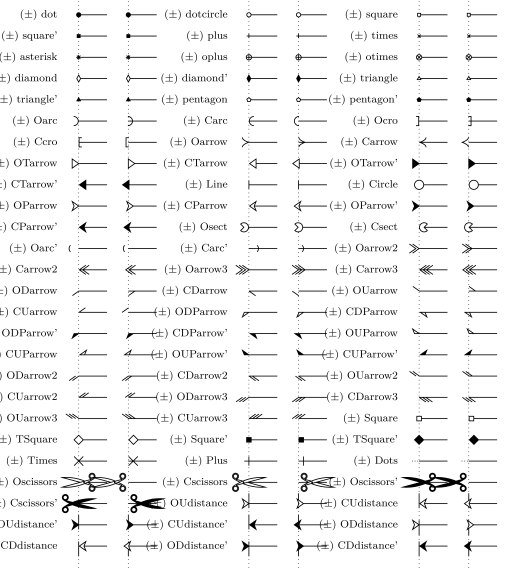
\includegraphics[]{marker.png}\else% TeXgraph version 2.0
\bgroup%
%\shorthandoff{;:!?}% uncomment if problem with babel
\pgfdeclarehorizontalshading[colorA,colorB]{myshading}{100bp}{color(0bp)=(colorA);color(75bp)=(colorB)}%
\pgfdeclareradialshading[colorA,colorB]{mysphereshading}{\pgfpoint{\GradCenterX bp}{\GradCenterY bp}}{color(0bp)=(colorA); color(35bp)=(colorB)}%
%\shorthandon{;:!?}% uncomment if problem with babel
\begin{tikzpicture}%
\pgfsetxvec{\pgfxy(0.75,0)}%
\pgfsetyvec{\pgfxy(0,0.75)}%
\useasboundingbox (-6,-15)--(12,5);
%objet1  (User)
\pgfsetstrokecolor{rgb,1:red,0;green,0;blue,0}%
\pgfsetlinewidth{0.6pt}%
\pgfsetroundcap%
\pgfsetroundjoin%
\pgfsetdash{{0pt}{3pt}}{0pt}%
\pgfxyline(-3.25,-15)(-3.25,5)%
\pgfxyline(-1.5,-15)(-1.5,5)%
\pgfxyline(2.75,-15)(2.75,5)%
\pgfxyline(4.5,-15)(4.5,5)%
\pgfxyline(8.75,-15)(8.75,5)%
\pgfxyline(10.5,-15)(10.5,5)%
\pgfputat{\pgfxy(-4,4.5)}{\pgftext[right]{\color{rgb,1:red,0;green,0;blue,0}\scriptsize ($\pm$) dot}}\pgfstroke%
\pgfsetbuttcap%
\pgfsetdash{}{0pt}%
\pgfxyline(-3.25,4.5)(-2.25,4.5)%
\pgfsetroundcap%
\pgfpathmoveto{\pgfxy(-3.175,4.5)}\pgfellipse{\pgfxy(-3.25,4.5)}{\pgfxy(0.0000,0.075)}{\pgfxy(-0.075,0.0000)}%
\pgfsetfillcolor{rgb,1:red,0;green,0;blue,0}%
\pgffillstroke%
\pgfsetbuttcap%
\pgfxyline(-1.5,4.5)(-0.5,4.5)%
\pgfsetroundcap%
\pgfpathmoveto{\pgfxy(-1.425,4.5)}\pgfellipse{\pgfxy(-1.5,4.5)}{\pgfxy(0.0000,0.075)}{\pgfxy(-0.075,0.0000)}%
\pgfsetfillcolor{rgb,1:red,0;green,0;blue,0}%
\pgffillstroke%
\pgfputat{\pgfxy(2,4.5)}{\pgftext[right]{\color{rgb,1:red,0;green,0;blue,0}\scriptsize ($\pm$) dotcircle}}\pgfstroke%
\pgfsetbuttcap%
\pgfxyline(2.75,4.5)(3.75,4.5)%
\pgfsetroundcap%
\pgfpathmoveto{\pgfxy(2.825,4.5)}\pgfellipse{\pgfxy(2.75,4.5)}{\pgfxy(0.0000,0.075)}{\pgfxy(-0.075,0.0000)}%
\pgfsetfillcolor{rgb,1:red,1;green,1;blue,1}%
\pgffillstroke%
\pgfsetbuttcap%
\pgfxyline(4.5,4.5)(5.5,4.5)%
\pgfsetroundcap%
\pgfpathmoveto{\pgfxy(4.575,4.5)}\pgfellipse{\pgfxy(4.5,4.5)}{\pgfxy(0.0000,0.075)}{\pgfxy(-0.075,0.0000)}%
\pgfsetfillcolor{rgb,1:red,1;green,1;blue,1}%
\pgffillstroke%
\pgfputat{\pgfxy(8,4.5)}{\pgftext[right]{\color{rgb,1:red,0;green,0;blue,0}\scriptsize ($\pm$) square}}\pgfstroke%
\pgfsetbuttcap%
\pgfxyline(8.75,4.5)(9.75,4.5)%
\pgfsetmiterjoin%
\pgfpathmoveto{\pgfxy(8.803,4.553)}%
\pgfpathlineto{\pgfxy(8.697,4.553)}\pgfpathlineto{\pgfxy(8.697,4.447)}\pgfpathlineto{\pgfxy(8.803,4.447)}\pgfclosepath%
\pgfsetfillcolor{rgb,1:red,1;green,1;blue,1}%
\pgffillstroke%
\pgfsetroundjoin%
\pgfxyline(10.5,4.5)(11.5,4.5)%
\pgfsetmiterjoin%
\pgfpathmoveto{\pgfxy(10.553,4.553)}%
\pgfpathlineto{\pgfxy(10.447,4.553)}\pgfpathlineto{\pgfxy(10.447,4.447)}\pgfpathlineto{\pgfxy(10.553,4.447)}\pgfclosepath%
\pgfsetfillcolor{rgb,1:red,1;green,1;blue,1}%
\pgffillstroke%
\pgfputat{\pgfxy(-4,3.75)}{\pgftext[right]{\color{rgb,1:red,0;green,0;blue,0}\scriptsize ($\pm$) square'}}\pgfstroke%
\pgfsetroundjoin%
\pgfxyline(-3.25,3.75)(-2.25,3.75)%
\pgfsetmiterjoin%
\pgfpathmoveto{\pgfxy(-3.197,3.803)}%
\pgfpathlineto{\pgfxy(-3.303,3.803)}\pgfpathlineto{\pgfxy(-3.303,3.697)}\pgfpathlineto{\pgfxy(-3.197,3.697)}\pgfclosepath%
\pgfsetfillcolor{rgb,1:red,0;green,0;blue,0}%
\pgffillstroke%
\pgfsetroundjoin%
\pgfxyline(-1.5,3.75)(-0.5,3.75)%
\pgfsetmiterjoin%
\pgfpathmoveto{\pgfxy(-1.447,3.803)}%
\pgfpathlineto{\pgfxy(-1.553,3.803)}\pgfpathlineto{\pgfxy(-1.553,3.697)}\pgfpathlineto{\pgfxy(-1.447,3.697)}\pgfclosepath%
\pgfsetfillcolor{rgb,1:red,0;green,0;blue,0}%
\pgffillstroke%
\pgfputat{\pgfxy(2,3.75)}{\pgftext[right]{\color{rgb,1:red,0;green,0;blue,0}\scriptsize ($\pm$) plus}}\pgfstroke%
\pgfsetroundjoin%
\pgfxyline(2.75,3.75)(3.75,3.75)%
\pgfxyline(2.825,3.75)(2.675,3.75)%
\pgfxyline(2.75,3.825)(2.75,3.675)%
\pgfxyline(4.5,3.75)(5.5,3.75)%
\pgfxyline(4.575,3.75)(4.425,3.75)%
\pgfxyline(4.5,3.825)(4.5,3.675)%
\pgfputat{\pgfxy(8,3.75)}{\pgftext[right]{\color{rgb,1:red,0;green,0;blue,0}\scriptsize ($\pm$) times}}\pgfstroke%
\pgfxyline(8.75,3.75)(9.75,3.75)%
\pgfsetmiterjoin%
\pgfxyline(8.803,3.803)(8.697,3.697)%
\pgfxyline(8.697,3.803)(8.803,3.697)%
\pgfsetroundjoin%
\pgfxyline(10.5,3.75)(11.5,3.75)%
\pgfsetmiterjoin%
\pgfxyline(10.553,3.803)(10.447,3.697)%
\pgfxyline(10.447,3.803)(10.553,3.697)%
\pgfputat{\pgfxy(-4,3)}{\pgftext[right]{\color{rgb,1:red,0;green,0;blue,0}\scriptsize ($\pm$) asterisk}}\pgfstroke%
\pgfsetroundjoin%
\pgfxyline(-3.25,3)(-2.25,3)%
\pgfsetroundcap%
\pgfxyline(-3.175,3)(-3.325,3)%
\pgfxyline(-3.25,3.075)(-3.25,2.925)%
\pgfxyline(-3.197,3.053)(-3.303,2.947)%
\pgfxyline(-3.303,3.053)(-3.197,2.947)%
\pgfsetbuttcap%
\pgfxyline(-1.5,3)(-0.5,3)%
\pgfsetroundcap%
\pgfxyline(-1.425,3)(-1.575,3)%
\pgfxyline(-1.5,3.075)(-1.5,2.925)%
\pgfxyline(-1.447,3.053)(-1.553,2.947)%
\pgfxyline(-1.553,3.053)(-1.447,2.947)%
\pgfputat{\pgfxy(2,3)}{\pgftext[right]{\color{rgb,1:red,0;green,0;blue,0}\scriptsize ($\pm$) oplus}}\pgfstroke%
\pgfsetbuttcap%
\pgfxyline(2.75,3)(3.75,3)%
\pgfsetroundcap%
\pgfpathmoveto{\pgfxy(2.8437,3)}\pgfellipse{\pgfxy(2.75,3)}{\pgfxy(0.0000,0.0937)}{\pgfxy(-0.0937,0.0000)}%
\pgfsetfillcolor{rgb,1:red,1;green,1;blue,1}%
\pgffillstroke%
\pgfsetbuttcap%
\pgfxyline(2.825,3)(2.675,3)%
\pgfxyline(2.75,3.075)(2.75,2.925)%
\pgfxyline(4.5,3)(5.5,3)%
\pgfsetroundcap%
\pgfpathmoveto{\pgfxy(4.5937,3)}\pgfellipse{\pgfxy(4.5,3)}{\pgfxy(0.0000,0.0937)}{\pgfxy(-0.0937,0.0000)}%
\pgfsetfillcolor{rgb,1:red,1;green,1;blue,1}%
\pgffillstroke%
\pgfsetbuttcap%
\pgfxyline(4.575,3)(4.425,3)%
\pgfxyline(4.5,3.075)(4.5,2.925)%
\pgfputat{\pgfxy(8,3)}{\pgftext[right]{\color{rgb,1:red,0;green,0;blue,0}\scriptsize ($\pm$) otimes}}\pgfstroke%
\pgfxyline(8.75,3)(9.75,3)%
\pgfsetroundcap%
\pgfsetmiterjoin%
\pgfpathmoveto{\pgfxy(8.8437,3)}\pgfellipse{\pgfxy(8.75,3)}{\pgfxy(0.0000,0.0937)}{\pgfxy(-0.0937,0.0000)}%
\pgfsetfillcolor{rgb,1:red,1;green,1;blue,1}%
\pgffillstroke%
\pgfsetbuttcap%
\pgfxyline(8.803,3.053)(8.697,2.947)%
\pgfxyline(8.697,3.053)(8.803,2.947)%
\pgfsetroundjoin%
\pgfxyline(10.5,3)(11.5,3)%
\pgfsetroundcap%
\pgfsetmiterjoin%
\pgfpathmoveto{\pgfxy(10.5937,3)}\pgfellipse{\pgfxy(10.5,3)}{\pgfxy(0.0000,0.0937)}{\pgfxy(-0.0937,0.0000)}%
\pgfsetfillcolor{rgb,1:red,1;green,1;blue,1}%
\pgffillstroke%
\pgfsetbuttcap%
\pgfxyline(10.553,3.053)(10.447,2.947)%
\pgfxyline(10.447,3.053)(10.553,2.947)%
\pgfputat{\pgfxy(-4,2.25)}{\pgftext[right]{\color{rgb,1:red,0;green,0;blue,0}\scriptsize ($\pm$) diamond}}\pgfstroke%
\pgfsetroundjoin%
\pgfxyline(-3.25,2.25)(-2.25,2.25)%
\pgfsetmiterjoin%
\pgfpathmoveto{\pgfxy(-3.25,2.3737)}%
\pgfpathlineto{\pgfxy(-3.3175,2.25)}\pgfpathlineto{\pgfxy(-3.25,2.1263)}\pgfpathlineto{\pgfxy(-3.1825,2.25)}\pgfclosepath%
\pgfsetfillcolor{rgb,1:red,1;green,1;blue,1}%
\pgffillstroke%
\pgfsetroundjoin%
\pgfxyline(-1.5,2.25)(-0.5,2.25)%
\pgfsetmiterjoin%
\pgfpathmoveto{\pgfxy(-1.5,2.3737)}%
\pgfpathlineto{\pgfxy(-1.5675,2.25)}\pgfpathlineto{\pgfxy(-1.5,2.1263)}\pgfpathlineto{\pgfxy(-1.4325,2.25)}\pgfclosepath%
\pgfsetfillcolor{rgb,1:red,1;green,1;blue,1}%
\pgffillstroke%
\pgfputat{\pgfxy(2,2.25)}{\pgftext[right]{\color{rgb,1:red,0;green,0;blue,0}\scriptsize ($\pm$) diamond'}}\pgfstroke%
\pgfsetroundjoin%
\pgfxyline(2.75,2.25)(3.75,2.25)%
\pgfsetmiterjoin%
\pgfpathmoveto{\pgfxy(2.75,2.3737)}%
\pgfpathlineto{\pgfxy(2.6825,2.25)}\pgfpathlineto{\pgfxy(2.75,2.1263)}\pgfpathlineto{\pgfxy(2.8175,2.25)}\pgfclosepath%
\pgfsetfillcolor{rgb,1:red,0;green,0;blue,0}%
\pgffillstroke%
\pgfsetroundjoin%
\pgfxyline(4.5,2.25)(5.5,2.25)%
\pgfsetmiterjoin%
\pgfpathmoveto{\pgfxy(4.5,2.3737)}%
\pgfpathlineto{\pgfxy(4.4325,2.25)}\pgfpathlineto{\pgfxy(4.5,2.1263)}\pgfpathlineto{\pgfxy(4.5675,2.25)}\pgfclosepath%
\pgfsetfillcolor{rgb,1:red,0;green,0;blue,0}%
\pgffillstroke%
\pgfputat{\pgfxy(8,2.25)}{\pgftext[right]{\color{rgb,1:red,0;green,0;blue,0}\scriptsize ($\pm$) triangle}}\pgfstroke%
\pgfsetroundjoin%
\pgfxyline(8.75,2.25)(9.75,2.25)%
\pgfsetmiterjoin%
\pgfpathmoveto{\pgfxy(8.75,2.325)}%
\pgfpathlineto{\pgfxy(8.6851,2.2125)}\pgfpathlineto{\pgfxy(8.8149,2.2125)}\pgfclosepath%
\pgfsetfillcolor{rgb,1:red,1;green,1;blue,1}%
\pgffillstroke%
\pgfsetroundjoin%
\pgfxyline(10.5,2.25)(11.5,2.25)%
\pgfsetmiterjoin%
\pgfpathmoveto{\pgfxy(10.5,2.325)}%
\pgfpathlineto{\pgfxy(10.4351,2.2125)}\pgfpathlineto{\pgfxy(10.5649,2.2125)}\pgfclosepath%
\pgfsetfillcolor{rgb,1:red,1;green,1;blue,1}%
\pgffillstroke%
\pgfputat{\pgfxy(-4,1.5)}{\pgftext[right]{\color{rgb,1:red,0;green,0;blue,0}\scriptsize ($\pm$) triangle'}}\pgfstroke%
\pgfsetroundjoin%
\pgfxyline(-3.25,1.5)(-2.25,1.5)%
\pgfsetmiterjoin%
\pgfpathmoveto{\pgfxy(-3.25,1.575)}%
\pgfpathlineto{\pgfxy(-3.3149,1.4625)}\pgfpathlineto{\pgfxy(-3.1851,1.4625)}\pgfclosepath%
\pgfsetfillcolor{rgb,1:red,0;green,0;blue,0}%
\pgffillstroke%
\pgfsetroundjoin%
\pgfxyline(-1.5,1.5)(-0.5,1.5)%
\pgfsetmiterjoin%
\pgfpathmoveto{\pgfxy(-1.5,1.575)}%
\pgfpathlineto{\pgfxy(-1.5649,1.4625)}\pgfpathlineto{\pgfxy(-1.4351,1.4625)}\pgfclosepath%
\pgfsetfillcolor{rgb,1:red,0;green,0;blue,0}%
\pgffillstroke%
\pgfputat{\pgfxy(2,1.5)}{\pgftext[right]{\color{rgb,1:red,0;green,0;blue,0}\scriptsize ($\pm$) pentagon}}\pgfstroke%
\pgfsetroundjoin%
\pgfxyline(2.75,1.5)(3.75,1.5)%
\pgfsetmiterjoin%
\pgfpathmoveto{\pgfxy(2.75,1.575)}%
\pgfpathlineto{\pgfxy(2.6787,1.5232)}\pgfpathlineto{\pgfxy(2.7059,1.4393)}\pgfpathlineto{\pgfxy(2.7941,1.4393)}\pgfpathlineto{\pgfxy(2.8213,1.5232)}%
\pgfclosepath%
\pgfsetfillcolor{rgb,1:red,1;green,1;blue,1}%
\pgffillstroke%
\pgfsetroundjoin%
\pgfxyline(4.5,1.5)(5.5,1.5)%
\pgfsetmiterjoin%
\pgfpathmoveto{\pgfxy(4.5,1.575)}%
\pgfpathlineto{\pgfxy(4.4287,1.5232)}\pgfpathlineto{\pgfxy(4.4559,1.4393)}\pgfpathlineto{\pgfxy(4.5441,1.4393)}\pgfpathlineto{\pgfxy(4.5713,1.5232)}%
\pgfclosepath%
\pgfsetfillcolor{rgb,1:red,1;green,1;blue,1}%
\pgffillstroke%
\pgfputat{\pgfxy(8,1.5)}{\pgftext[right]{\color{rgb,1:red,0;green,0;blue,0}\scriptsize ($\pm$) pentagon'}}\pgfstroke%
\pgfsetroundjoin%
\pgfxyline(8.75,1.5)(9.75,1.5)%
\pgfsetmiterjoin%
\pgfpathmoveto{\pgfxy(8.75,1.575)}%
\pgfpathlineto{\pgfxy(8.6787,1.5232)}\pgfpathlineto{\pgfxy(8.7059,1.4393)}\pgfpathlineto{\pgfxy(8.7941,1.4393)}\pgfpathlineto{\pgfxy(8.8213,1.5232)}%
\pgfclosepath%
\pgfsetfillcolor{rgb,1:red,0;green,0;blue,0}%
\pgffillstroke%
\pgfsetroundjoin%
\pgfxyline(10.5,1.5)(11.5,1.5)%
\pgfsetmiterjoin%
\pgfpathmoveto{\pgfxy(10.5,1.575)}%
\pgfpathlineto{\pgfxy(10.4287,1.5232)}\pgfpathlineto{\pgfxy(10.4559,1.4393)}\pgfpathlineto{\pgfxy(10.5441,1.4393)}\pgfpathlineto{\pgfxy(10.5713,1.5232)}%
\pgfclosepath%
\pgfsetfillcolor{rgb,1:red,0;green,0;blue,0}%
\pgffillstroke%
\pgfputat{\pgfxy(-4,0.75)}{\pgftext[right]{\color{rgb,1:red,0;green,0;blue,0}\scriptsize ($\pm$) Oarc}}\pgfstroke%
\pgfsetroundjoin%
\pgfxyline(-3.25,0.75)(-2.25,0.75)%
\pgfpathmoveto{\pgfxy(-3.4262,0.5881)}\pgfpatharc{-90}{90}{0.1214cm}%
\pgfstroke%
\pgfxyline(-1.5,0.75)(-0.5,0.75)%
\pgfpathmoveto{\pgfxy(-1.5143,0.5881)}\pgfpatharc{-90}{90}{0.1214cm}%
\pgfstroke%
\pgfputat{\pgfxy(2,0.75)}{\pgftext[right]{\color{rgb,1:red,0;green,0;blue,0}\scriptsize ($\pm$) Carc}}\pgfstroke%
\pgfxyline(2.75,0.75)(3.75,0.75)%
\pgfpathmoveto{\pgfxy(2.9262,0.9119)}\pgfpatharc{90}{270}{0.1214cm}%
\pgfstroke%
\pgfxyline(4.5,0.75)(5.5,0.75)%
\pgfpathmoveto{\pgfxy(4.5143,0.9119)}\pgfpatharc{90}{270}{0.1214cm}%
\pgfstroke%
\pgfputat{\pgfxy(8,0.75)}{\pgftext[right]{\color{rgb,1:red,0;green,0;blue,0}\scriptsize ($\pm$) Ocro}}\pgfstroke%
\pgfxyline(8.75,0.75)(9.75,0.75)%
\pgfsetmiterjoin%
\pgfpathmoveto{\pgfxy(8.6405,0.9119)}%
\pgfpathlineto{\pgfxy(8.7357,0.9119)}\pgfpathlineto{\pgfxy(8.7357,0.5881)}\pgfpathlineto{\pgfxy(8.6405,0.5881)}%
\pgfstroke%
\pgfsetroundjoin%
\pgfxyline(10.5,0.75)(11.5,0.75)%
\pgfsetmiterjoin%
\pgfpathmoveto{\pgfxy(10.4857,0.9119)}%
\pgfpathlineto{\pgfxy(10.581,0.9119)}\pgfpathlineto{\pgfxy(10.581,0.5881)}\pgfpathlineto{\pgfxy(10.4857,0.5881)}%
\pgfstroke%
\pgfputat{\pgfxy(-4,0)}{\pgftext[right]{\color{rgb,1:red,0;green,0;blue,0}\scriptsize ($\pm$) Ccro}}\pgfstroke%
\pgfsetroundjoin%
\pgfxyline(-3.25,0)(-2.25,0)%
\pgfsetmiterjoin%
\pgfpathmoveto{\pgfxy(-3.1405,0.1619)}%
\pgfpathlineto{\pgfxy(-3.2357,0.1619)}\pgfpathlineto{\pgfxy(-3.2357,-0.1619)}\pgfpathlineto{\pgfxy(-3.1405,-0.1619)}%
\pgfstroke%
\pgfsetroundjoin%
\pgfxyline(-1.5,0)(-0.5,0)%
\pgfsetmiterjoin%
\pgfpathmoveto{\pgfxy(-1.4857,0.1619)}%
\pgfpathlineto{\pgfxy(-1.581,0.1619)}\pgfpathlineto{\pgfxy(-1.581,-0.1619)}\pgfpathlineto{\pgfxy(-1.4857,-0.1619)}%
\pgfstroke%
\pgfputat{\pgfxy(2,0)}{\pgftext[right]{\color{rgb,1:red,0;green,0;blue,0}\scriptsize ($\pm$) Oarrow}}\pgfstroke%
\pgfsetroundjoin%
\pgfxyline(2.75,0)(3.75,0)%
\pgfsetroundcap%
\pgfpathmoveto{\pgfxy(2.5214,-0.1619)}%
\pgfpathcurveto{\pgfxy(2.5214,-0.081)}{\pgfxy(2.7214,0)}{\pgfxy(2.75,0)}%
\pgfpathcurveto{\pgfxy(2.7214,0)}{\pgfxy(2.5214,0.081)}{\pgfxy(2.5214,0.1619)}%
\pgfstroke%
\pgfsetbuttcap%
\pgfxyline(4.5,0)(5.5,0)%
\pgfsetroundcap%
\pgfpathmoveto{\pgfxy(4.5143,-0.1619)}%
\pgfpathcurveto{\pgfxy(4.5143,-0.081)}{\pgfxy(4.7143,0)}{\pgfxy(4.7429,0)}%
\pgfpathcurveto{\pgfxy(4.7143,0)}{\pgfxy(4.5143,0.081)}{\pgfxy(4.5143,0.1619)}%
\pgfstroke%
\pgfputat{\pgfxy(8,0)}{\pgftext[right]{\color{rgb,1:red,0;green,0;blue,0}\scriptsize ($\pm$) Carrow}}\pgfstroke%
\pgfsetbuttcap%
\pgfxyline(8.7908,0)(9.75,0)%
\pgfsetroundcap%
\pgfpathmoveto{\pgfxy(8.9929,-0.1619)}%
\pgfpathcurveto{\pgfxy(8.9929,-0.081)}{\pgfxy(8.7929,0)}{\pgfxy(8.7643,0)}%
\pgfpathcurveto{\pgfxy(8.7929,0)}{\pgfxy(8.9929,0.081)}{\pgfxy(8.9929,0.1619)}%
\pgfstroke%
\pgfsetbuttcap%
\pgfxyline(10.5,0)(11.5,0)%
\pgfsetroundcap%
\pgfpathmoveto{\pgfxy(10.4857,-0.1619)}%
\pgfpathcurveto{\pgfxy(10.4857,-0.081)}{\pgfxy(10.2857,0)}{\pgfxy(10.2571,0)}%
\pgfpathcurveto{\pgfxy(10.2857,0)}{\pgfxy(10.4857,0.081)}{\pgfxy(10.4857,0.1619)}%
\pgfstroke%
\pgfputat{\pgfxy(-4,-0.75)}{\pgftext[right]{\color{rgb,1:red,0;green,0;blue,0}\scriptsize ($\pm$) OTarrow}}\pgfstroke%
\pgfsetbuttcap%
\pgfxyline(-3.25,-0.75)(-2.25,-0.75)%
\pgfsetmiterjoin%
\pgfpathmoveto{\pgfxy(-3.25,-0.75)}%
\pgfpathlineto{\pgfxy(-3.4786,-0.5881)}\pgfpathlineto{\pgfxy(-3.4786,-0.9119)}\pgfclosepath%
\pgfsetfillcolor{rgb,1:red,1;green,1;blue,1}%
\pgffillstroke%
\pgfsetroundjoin%
\pgfxyline(-1.5,-0.75)(-0.5,-0.75)%
\pgfsetmiterjoin%
\pgfpathmoveto{\pgfxy(-1.2714,-0.75)}%
\pgfpathlineto{\pgfxy(-1.5,-0.5881)}\pgfpathlineto{\pgfxy(-1.5,-0.9119)}\pgfclosepath%
\pgfsetfillcolor{rgb,1:red,1;green,1;blue,1}%
\pgffillstroke%
\pgfputat{\pgfxy(2,-0.75)}{\pgftext[right]{\color{rgb,1:red,0;green,0;blue,0}\scriptsize ($\pm$) CTarrow}}\pgfstroke%
\pgfsetroundjoin%
\pgfxyline(2.7908,-0.75)(3.75,-0.75)%
\pgfsetmiterjoin%
\pgfpathmoveto{\pgfxy(2.7747,-0.75)}%
\pgfpathlineto{\pgfxy(3.0033,-0.5881)}\pgfpathlineto{\pgfxy(3.0033,-0.9119)}\pgfclosepath%
\pgfsetfillcolor{rgb,1:red,1;green,1;blue,1}%
\pgffillstroke%
\pgfsetroundjoin%
\pgfxyline(4.5,-0.75)(5.5,-0.75)%
\pgfsetmiterjoin%
\pgfpathmoveto{\pgfxy(4.2961,-0.75)}%
\pgfpathlineto{\pgfxy(4.5247,-0.5881)}\pgfpathlineto{\pgfxy(4.5247,-0.9119)}\pgfclosepath%
\pgfsetfillcolor{rgb,1:red,1;green,1;blue,1}%
\pgffillstroke%
\pgfputat{\pgfxy(8,-0.75)}{\pgftext[right]{\color{rgb,1:red,0;green,0;blue,0}\scriptsize ($\pm$) OTarrow'}}\pgfstroke%
\pgfsetroundjoin%
\pgfxyline(8.75,-0.75)(9.75,-0.75)%
\pgfsetmiterjoin%
\pgfpathmoveto{\pgfxy(8.75,-0.75)}%
\pgfpathlineto{\pgfxy(8.5214,-0.5881)}\pgfpathlineto{\pgfxy(8.5214,-0.9119)}\pgfclosepath%
\pgfsetfillcolor{rgb,1:red,0;green,0;blue,0}%
\pgffillstroke%
\pgfsetroundjoin%
\pgfxyline(10.5,-0.75)(11.5,-0.75)%
\pgfsetmiterjoin%
\pgfpathmoveto{\pgfxy(10.7286,-0.75)}%
\pgfpathlineto{\pgfxy(10.5,-0.5881)}\pgfpathlineto{\pgfxy(10.5,-0.9119)}\pgfclosepath%
\pgfsetfillcolor{rgb,1:red,0;green,0;blue,0}%
\pgffillstroke%
\pgfputat{\pgfxy(-4,-1.5)}{\pgftext[right]{\color{rgb,1:red,0;green,0;blue,0}\scriptsize ($\pm$) CTarrow'}}\pgfstroke%
\pgfsetroundjoin%
\pgfxyline(-3.2092,-1.5)(-2.25,-1.5)%
\pgfsetmiterjoin%
\pgfpathmoveto{\pgfxy(-3.2253,-1.5)}%
\pgfpathlineto{\pgfxy(-2.9967,-1.3381)}\pgfpathlineto{\pgfxy(-2.9967,-1.6619)}\pgfclosepath%
\pgfsetfillcolor{rgb,1:red,0;green,0;blue,0}%
\pgffillstroke%
\pgfsetroundjoin%
\pgfxyline(-1.5,-1.5)(-0.5,-1.5)%
\pgfsetmiterjoin%
\pgfpathmoveto{\pgfxy(-1.7039,-1.5)}%
\pgfpathlineto{\pgfxy(-1.4753,-1.3381)}\pgfpathlineto{\pgfxy(-1.4753,-1.6619)}\pgfclosepath%
\pgfsetfillcolor{rgb,1:red,0;green,0;blue,0}%
\pgffillstroke%
\pgfputat{\pgfxy(2,-1.5)}{\pgftext[right]{\color{rgb,1:red,0;green,0;blue,0}\scriptsize ($\pm$) Line}}\pgfstroke%
\pgfsetroundjoin%
\pgfxyline(2.75,-1.5)(3.75,-1.5)%
\pgfxyline(2.75,-1.3381)(2.75,-1.6619)%
\pgfxyline(4.5,-1.5)(5.5,-1.5)%
\pgfxyline(4.5,-1.3381)(4.5,-1.6619)%
\pgfputat{\pgfxy(8,-1.5)}{\pgftext[right]{\color{rgb,1:red,0;green,0;blue,0}\scriptsize ($\pm$) Circle}}\pgfstroke%
\pgfxyline(8.75,-1.5)(9.75,-1.5)%
\pgfellipse{\pgfxy(8.75,-1.5)}{\pgfxy(0.0000,0.1619)}{\pgfxy(-0.1619,0.0000)}%
\pgfsetfillcolor{rgb,1:red,1;green,1;blue,1}%
\pgffillstroke%
\pgfxyline(10.5408,-1.5)(11.5,-1.5)%
\pgfellipse{\pgfxy(10.6762,-1.5)}{\pgfxy(0.0000,0.1619)}{\pgfxy(-0.1619,0.0000)}%
\pgfsetfillcolor{rgb,1:red,1;green,1;blue,1}%
\pgffillstroke%
\pgfputat{\pgfxy(-4,-2.25)}{\pgftext[right]{\color{rgb,1:red,0;green,0;blue,0}\scriptsize ($\pm$) OParrow}}\pgfstroke%
\pgfxyline(-3.25,-2.25)(-2.25,-2.25)%
\pgfsetmiterjoin%
\pgfpathmoveto{\pgfxy(-3.25,-2.25)}%
\pgfpathlineto{\pgfxy(-3.4786,-2.4119)}\pgfpathlineto{\pgfxy(-3.4119,-2.25)}\pgfpathlineto{\pgfxy(-3.4786,-2.0881)}\pgfclosepath%
\pgfsetfillcolor{rgb,1:red,1;green,1;blue,1}%
\pgffillstroke%
\pgfsetroundjoin%
\pgfxyline(-1.5,-2.25)(-0.5,-2.25)%
\pgfsetmiterjoin%
\pgfpathmoveto{\pgfxy(-1.3238,-2.25)}%
\pgfpathlineto{\pgfxy(-1.5524,-2.4119)}\pgfpathlineto{\pgfxy(-1.4857,-2.25)}\pgfpathlineto{\pgfxy(-1.5524,-2.0881)}\pgfclosepath%
\pgfsetfillcolor{rgb,1:red,1;green,1;blue,1}%
\pgffillstroke%
\pgfputat{\pgfxy(2,-2.25)}{\pgftext[right]{\color{rgb,1:red,0;green,0;blue,0}\scriptsize ($\pm$) CParrow}}\pgfstroke%
\pgfsetroundjoin%
\pgfxyline(2.7908,-2.25)(3.75,-2.25)%
\pgfsetmiterjoin%
\pgfpathmoveto{\pgfxy(2.7747,-2.25)}%
\pgfpathlineto{\pgfxy(3.0033,-2.4119)}\pgfpathlineto{\pgfxy(2.9366,-2.25)}\pgfpathlineto{\pgfxy(3.0033,-2.0881)}\pgfclosepath%
\pgfsetfillcolor{rgb,1:red,1;green,1;blue,1}%
\pgffillstroke%
\pgfsetroundjoin%
\pgfxyline(4.5,-2.25)(5.5,-2.25)%
\pgfsetmiterjoin%
\pgfpathmoveto{\pgfxy(4.3485,-2.25)}%
\pgfpathlineto{\pgfxy(4.5771,-2.4119)}\pgfpathlineto{\pgfxy(4.5104,-2.25)}\pgfpathlineto{\pgfxy(4.5771,-2.0881)}\pgfclosepath%
\pgfsetfillcolor{rgb,1:red,1;green,1;blue,1}%
\pgffillstroke%
\pgfputat{\pgfxy(8,-2.25)}{\pgftext[right]{\color{rgb,1:red,0;green,0;blue,0}\scriptsize ($\pm$) OParrow'}}\pgfstroke%
\pgfsetroundjoin%
\pgfxyline(8.75,-2.25)(9.75,-2.25)%
\pgfsetmiterjoin%
\pgfpathmoveto{\pgfxy(8.75,-2.25)}%
\pgfpathlineto{\pgfxy(8.5214,-2.4119)}\pgfpathlineto{\pgfxy(8.5881,-2.25)}\pgfpathlineto{\pgfxy(8.5214,-2.0881)}\pgfclosepath%
\pgfsetfillcolor{rgb,1:red,0;green,0;blue,0}%
\pgffillstroke%
\pgfsetroundjoin%
\pgfxyline(10.5,-2.25)(11.5,-2.25)%
\pgfsetmiterjoin%
\pgfpathmoveto{\pgfxy(10.6762,-2.25)}%
\pgfpathlineto{\pgfxy(10.4476,-2.4119)}\pgfpathlineto{\pgfxy(10.5143,-2.25)}\pgfpathlineto{\pgfxy(10.4476,-2.0881)}\pgfclosepath%
\pgfsetfillcolor{rgb,1:red,0;green,0;blue,0}%
\pgffillstroke%
\pgfputat{\pgfxy(-4,-3)}{\pgftext[right]{\color{rgb,1:red,0;green,0;blue,0}\scriptsize ($\pm$) CParrow'}}\pgfstroke%
\pgfsetroundjoin%
\pgfxyline(-3.2092,-3)(-2.25,-3)%
\pgfsetmiterjoin%
\pgfpathmoveto{\pgfxy(-3.2253,-3)}%
\pgfpathlineto{\pgfxy(-2.9967,-3.1619)}\pgfpathlineto{\pgfxy(-3.0634,-3)}\pgfpathlineto{\pgfxy(-2.9967,-2.8381)}\pgfclosepath%
\pgfsetfillcolor{rgb,1:red,0;green,0;blue,0}%
\pgffillstroke%
\pgfsetroundjoin%
\pgfxyline(-1.5,-3)(-0.5,-3)%
\pgfsetmiterjoin%
\pgfpathmoveto{\pgfxy(-1.6515,-3)}%
\pgfpathlineto{\pgfxy(-1.4229,-3.1619)}\pgfpathlineto{\pgfxy(-1.4896,-3)}\pgfpathlineto{\pgfxy(-1.4229,-2.8381)}\pgfclosepath%
\pgfsetfillcolor{rgb,1:red,0;green,0;blue,0}%
\pgffillstroke%
\pgfputat{\pgfxy(2,-3)}{\pgftext[right]{\color{rgb,1:red,0;green,0;blue,0}\scriptsize ($\pm$) Osect}}\pgfstroke%
\pgfsetroundjoin%
\pgfxyline(2.75,-3)(3.75,-3)%
\pgfsetmiterjoin%
\pgfpathmoveto{\pgfxy(2.4593,-3.1145)}\pgfpatharc{-135}{135}{0.1214cm}%
\pgfpathlineto{\pgfxy(2.5738,-3)}%
\pgfclosepath%
\pgfsetfillcolor{rgb,1:red,1;green,1;blue,1}%
\pgffillstroke%
\pgfsetroundjoin%
\pgfxyline(4.5,-3)(5.5,-3)%
\pgfsetmiterjoin%
\pgfpathmoveto{\pgfxy(4.3712,-3.1145)}\pgfpatharc{-135}{135}{0.1214cm}%
\pgfpathlineto{\pgfxy(4.4857,-3)}%
\pgfclosepath%
\pgfsetfillcolor{rgb,1:red,1;green,1;blue,1}%
\pgffillstroke%
\pgfputat{\pgfxy(8,-3)}{\pgftext[right]{\color{rgb,1:red,0;green,0;blue,0}\scriptsize ($\pm$) Csect}}\pgfstroke%
\pgfsetroundjoin%
\pgfxyline(8.7908,-3)(9.75,-3)%
\pgfsetmiterjoin%
\pgfpathmoveto{\pgfxy(9.0407,-2.8855)}\pgfpatharc{45}{315}{0.1214cm}%
\pgfpathlineto{\pgfxy(8.9262,-3)}%
\pgfclosepath%
\pgfsetfillcolor{rgb,1:red,1;green,1;blue,1}%
\pgffillstroke%
\pgfsetroundjoin%
\pgfxyline(10.5,-3)(11.5,-3)%
\pgfsetmiterjoin%
\pgfpathmoveto{\pgfxy(10.6288,-2.8855)}\pgfpatharc{45}{315}{0.1214cm}%
\pgfpathlineto{\pgfxy(10.5143,-3)}%
\pgfclosepath%
\pgfsetfillcolor{rgb,1:red,1;green,1;blue,1}%
\pgffillstroke%
\pgfputat{\pgfxy(-4,-3.75)}{\pgftext[right]{\color{rgb,1:red,0;green,0;blue,0}\scriptsize ($\pm$) Oarc'}}\pgfstroke%
\pgfsetroundjoin%
\pgfxyline(-3.25,-3.75)(-2.25,-3.75)%
\pgfpathmoveto{\pgfxy(-3.5407,-3.8645)}\pgfpatharc{-135}{135}{0.1214cm}%
\pgfstroke%
\pgfxyline(-1.5,-3.75)(-0.5,-3.75)%
\pgfpathmoveto{\pgfxy(-1.6288,-3.8645)}\pgfpatharc{-135}{135}{0.1214cm}%
\pgfstroke%
\pgfputat{\pgfxy(2,-3.75)}{\pgftext[right]{\color{rgb,1:red,0;green,0;blue,0}\scriptsize ($\pm$) Carc'}}\pgfstroke%
\pgfxyline(2.75,-3.75)(3.75,-3.75)%
\pgfpathmoveto{\pgfxy(3.0407,-3.6355)}\pgfpatharc{45}{315}{0.1214cm}%
\pgfstroke%
\pgfxyline(4.5,-3.75)(5.5,-3.75)%
\pgfpathmoveto{\pgfxy(4.6288,-3.6355)}\pgfpatharc{45}{315}{0.1214cm}%
\pgfstroke%
\pgfputat{\pgfxy(8,-3.75)}{\pgftext[right]{\color{rgb,1:red,0;green,0;blue,0}\scriptsize ($\pm$) Oarrow2}}\pgfstroke%
\pgfxyline(8.75,-3.75)(9.75,-3.75)%
\pgfsetmiterjoin%
\pgfpathmoveto{\pgfxy(8.5214,-3.9119)}%
\pgfpathlineto{\pgfxy(8.75,-3.75)}\pgfpathlineto{\pgfxy(8.5214,-3.5881)}%
\pgfstroke%
\pgfpathmoveto{\pgfxy(8.4053,-3.9119)}%
\pgfpathlineto{\pgfxy(8.6339,-3.75)}\pgfpathlineto{\pgfxy(8.4053,-3.5881)}%
\pgfstroke%
\pgfsetroundjoin%
\pgfxyline(10.5,-3.75)(11.5,-3.75)%
\pgfsetmiterjoin%
\pgfpathmoveto{\pgfxy(10.3875,-3.9119)}%
\pgfpathlineto{\pgfxy(10.6161,-3.75)}\pgfpathlineto{\pgfxy(10.3875,-3.5881)}%
\pgfstroke%
\pgfpathmoveto{\pgfxy(10.2714,-3.9119)}%
\pgfpathlineto{\pgfxy(10.5,-3.75)}\pgfpathlineto{\pgfxy(10.2714,-3.5881)}%
\pgfstroke%
\pgfputat{\pgfxy(-4,-4.5)}{\pgftext[right]{\color{rgb,1:red,0;green,0;blue,0}\scriptsize ($\pm$) Carrow2}}\pgfstroke%
\pgfsetroundjoin%
\pgfxyline(-3.2092,-4.5)(-2.25,-4.5)%
\pgfsetmiterjoin%
\pgfpathmoveto{\pgfxy(-2.9967,-4.6619)}%
\pgfpathlineto{\pgfxy(-3.2253,-4.5)}\pgfpathlineto{\pgfxy(-2.9967,-4.3381)}%
\pgfstroke%
\pgfpathmoveto{\pgfxy(-2.8806,-4.6619)}%
\pgfpathlineto{\pgfxy(-3.1092,-4.5)}\pgfpathlineto{\pgfxy(-2.8806,-4.3381)}%
\pgfstroke%
\pgfsetroundjoin%
\pgfxyline(-1.4592,-4.5)(-0.5,-4.5)%
\pgfsetmiterjoin%
\pgfpathmoveto{\pgfxy(-1.3628,-4.6619)}%
\pgfpathlineto{\pgfxy(-1.5914,-4.5)}\pgfpathlineto{\pgfxy(-1.3628,-4.3381)}%
\pgfstroke%
\pgfpathmoveto{\pgfxy(-1.2467,-4.6619)}%
\pgfpathlineto{\pgfxy(-1.4753,-4.5)}\pgfpathlineto{\pgfxy(-1.2467,-4.3381)}%
\pgfstroke%
\pgfputat{\pgfxy(2,-4.5)}{\pgftext[right]{\color{rgb,1:red,0;green,0;blue,0}\scriptsize ($\pm$) Oarrow3}}\pgfstroke%
\pgfsetroundjoin%
\pgfxyline(2.75,-4.5)(3.75,-4.5)%
\pgfsetmiterjoin%
\pgfpathmoveto{\pgfxy(2.5214,-4.6619)}%
\pgfpathlineto{\pgfxy(2.75,-4.5)}\pgfpathlineto{\pgfxy(2.5214,-4.3381)}%
\pgfstroke%
\pgfpathmoveto{\pgfxy(2.4053,-4.6619)}%
\pgfpathlineto{\pgfxy(2.6339,-4.5)}\pgfpathlineto{\pgfxy(2.4053,-4.3381)}%
\pgfstroke%
\pgfpathmoveto{\pgfxy(2.2892,-4.6619)}%
\pgfpathlineto{\pgfxy(2.5178,-4.5)}\pgfpathlineto{\pgfxy(2.2892,-4.3381)}%
\pgfstroke%
\pgfsetroundjoin%
\pgfxyline(4.5,-4.5)(5.5,-4.5)%
\pgfsetmiterjoin%
\pgfpathmoveto{\pgfxy(4.5036,-4.6619)}%
\pgfpathlineto{\pgfxy(4.7322,-4.5)}\pgfpathlineto{\pgfxy(4.5036,-4.3381)}%
\pgfstroke%
\pgfpathmoveto{\pgfxy(4.3875,-4.6619)}%
\pgfpathlineto{\pgfxy(4.6161,-4.5)}\pgfpathlineto{\pgfxy(4.3875,-4.3381)}%
\pgfstroke%
\pgfpathmoveto{\pgfxy(4.2714,-4.6619)}%
\pgfpathlineto{\pgfxy(4.5,-4.5)}\pgfpathlineto{\pgfxy(4.2714,-4.3381)}%
\pgfstroke%
\pgfputat{\pgfxy(8,-4.5)}{\pgftext[right]{\color{rgb,1:red,0;green,0;blue,0}\scriptsize ($\pm$) Carrow3}}\pgfstroke%
\pgfsetroundjoin%
\pgfxyline(8.7908,-4.5)(9.75,-4.5)%
\pgfsetmiterjoin%
\pgfpathmoveto{\pgfxy(9.0033,-4.6619)}%
\pgfpathlineto{\pgfxy(8.7747,-4.5)}\pgfpathlineto{\pgfxy(9.0033,-4.3381)}%
\pgfstroke%
\pgfpathmoveto{\pgfxy(9.1194,-4.6619)}%
\pgfpathlineto{\pgfxy(8.8908,-4.5)}\pgfpathlineto{\pgfxy(9.1194,-4.3381)}%
\pgfstroke%
\pgfpathmoveto{\pgfxy(9.2355,-4.6619)}%
\pgfpathlineto{\pgfxy(9.0069,-4.5)}\pgfpathlineto{\pgfxy(9.2355,-4.3381)}%
\pgfstroke%
\pgfsetroundjoin%
\pgfxyline(10.5408,-4.5)(11.5,-4.5)%
\pgfsetmiterjoin%
\pgfpathmoveto{\pgfxy(10.5211,-4.6619)}%
\pgfpathlineto{\pgfxy(10.2925,-4.5)}\pgfpathlineto{\pgfxy(10.5211,-4.3381)}%
\pgfstroke%
\pgfpathmoveto{\pgfxy(10.6372,-4.6619)}%
\pgfpathlineto{\pgfxy(10.4086,-4.5)}\pgfpathlineto{\pgfxy(10.6372,-4.3381)}%
\pgfstroke%
\pgfpathmoveto{\pgfxy(10.7533,-4.6619)}%
\pgfpathlineto{\pgfxy(10.5247,-4.5)}\pgfpathlineto{\pgfxy(10.7533,-4.3381)}%
\pgfstroke%
\pgfputat{\pgfxy(-4,-5.25)}{\pgftext[right]{\color{rgb,1:red,0;green,0;blue,0}\scriptsize ($\pm$) ODarrow}}\pgfstroke%
\pgfsetroundjoin%
\pgfxyline(-3.25,-5.25)(-2.25,-5.25)%
\pgfsetmiterjoin%
\pgfxyline(-3.2417,-5.2474)(-3.4703,-5.4093)%
\pgfsetroundjoin%
\pgfxyline(-1.5,-5.25)(-0.5,-5.25)%
\pgfsetmiterjoin%
\pgfxyline(-1.2632,-5.2474)(-1.4917,-5.4093)%
\pgfputat{\pgfxy(2,-5.25)}{\pgftext[right]{\color{rgb,1:red,0;green,0;blue,0}\scriptsize ($\pm$) CDarrow}}\pgfstroke%
\pgfsetroundjoin%
\pgfxyline(2.75,-5.25)(3.75,-5.25)%
\pgfsetmiterjoin%
\pgfxyline(2.7583,-5.2526)(2.9868,-5.4145)%
\pgfsetroundjoin%
\pgfxyline(4.5,-5.25)(5.5,-5.25)%
\pgfsetmiterjoin%
\pgfxyline(4.2797,-5.2526)(4.5083,-5.4145)%
\pgfputat{\pgfxy(8,-5.25)}{\pgftext[right]{\color{rgb,1:red,0;green,0;blue,0}\scriptsize ($\pm$) OUarrow}}\pgfstroke%
\pgfsetroundjoin%
\pgfxyline(8.75,-5.25)(9.75,-5.25)%
\pgfsetmiterjoin%
\pgfxyline(8.7583,-5.2474)(8.5297,-5.0855)%
\pgfsetroundjoin%
\pgfxyline(10.5,-5.25)(11.5,-5.25)%
\pgfsetmiterjoin%
\pgfxyline(10.7368,-5.2474)(10.5083,-5.0855)%
\pgfputat{\pgfxy(-4,-6)}{\pgftext[right]{\color{rgb,1:red,0;green,0;blue,0}\scriptsize ($\pm$) CUarrow}}\pgfstroke%
\pgfsetroundjoin%
\pgfxyline(-3.25,-6)(-2.25,-6)%
\pgfsetmiterjoin%
\pgfxyline(-3.2417,-6.0026)(-3.0132,-5.8407)%
\pgfsetroundjoin%
\pgfxyline(-1.5,-6)(-0.5,-6)%
\pgfsetmiterjoin%
\pgfxyline(-1.7203,-6.0026)(-1.4917,-5.8407)%
\pgfputat{\pgfxy(2,-6)}{\pgftext[right]{\color{rgb,1:red,0;green,0;blue,0}\scriptsize ($\pm$) ODParrow}}\pgfstroke%
\pgfsetroundjoin%
\pgfxyline(2.75,-6)(3.75,-6)%
\pgfsetmiterjoin%
\pgfpathmoveto{\pgfxy(2.75,-6)}%
\pgfpathlineto{\pgfxy(2.5881,-6)}\pgfpathlineto{\pgfxy(2.5214,-6.1619)}\pgfclosepath%
\pgfsetfillcolor{rgb,1:red,1;green,1;blue,1}%
\pgffillstroke%
\pgfsetroundjoin%
\pgfxyline(4.5,-6)(5.5,-6)%
\pgfsetmiterjoin%
\pgfpathmoveto{\pgfxy(4.6762,-6)}%
\pgfpathlineto{\pgfxy(4.5143,-6)}\pgfpathlineto{\pgfxy(4.4476,-6.1619)}\pgfclosepath%
\pgfsetfillcolor{rgb,1:red,1;green,1;blue,1}%
\pgffillstroke%
\pgfputat{\pgfxy(8,-6)}{\pgftext[right]{\color{rgb,1:red,0;green,0;blue,0}\scriptsize ($\pm$) CDParrow}}\pgfstroke%
\pgfsetroundjoin%
\pgfxyline(8.7908,-6)(9.75,-6)%
\pgfsetmiterjoin%
\pgfpathmoveto{\pgfxy(8.7949,-6)}%
\pgfpathlineto{\pgfxy(8.9568,-6)}\pgfpathlineto{\pgfxy(9.0235,-6.1619)}\pgfclosepath%
\pgfsetfillcolor{rgb,1:red,1;green,1;blue,1}%
\pgffillstroke%
\pgfsetroundjoin%
\pgfxyline(10.5,-6)(11.5,-6)%
\pgfsetmiterjoin%
\pgfpathmoveto{\pgfxy(10.3687,-6)}%
\pgfpathlineto{\pgfxy(10.5306,-6)}\pgfpathlineto{\pgfxy(10.5973,-6.1619)}\pgfclosepath%
\pgfsetfillcolor{rgb,1:red,1;green,1;blue,1}%
\pgffillstroke%
\pgfputat{\pgfxy(-4,-6.75)}{\pgftext[right]{\color{rgb,1:red,0;green,0;blue,0}\scriptsize ($\pm$) ODParrow'}}\pgfstroke%
\pgfsetroundjoin%
\pgfxyline(-3.25,-6.75)(-2.25,-6.75)%
\pgfsetmiterjoin%
\pgfpathmoveto{\pgfxy(-3.25,-6.75)}%
\pgfpathlineto{\pgfxy(-3.4119,-6.75)}\pgfpathlineto{\pgfxy(-3.4786,-6.9119)}\pgfclosepath%
\pgfsetfillcolor{rgb,1:red,0;green,0;blue,0}%
\pgffillstroke%
\pgfsetroundjoin%
\pgfxyline(-1.5,-6.75)(-0.5,-6.75)%
\pgfsetmiterjoin%
\pgfpathmoveto{\pgfxy(-1.3238,-6.75)}%
\pgfpathlineto{\pgfxy(-1.4857,-6.75)}\pgfpathlineto{\pgfxy(-1.5524,-6.9119)}\pgfclosepath%
\pgfsetfillcolor{rgb,1:red,0;green,0;blue,0}%
\pgffillstroke%
\pgfputat{\pgfxy(2,-6.75)}{\pgftext[right]{\color{rgb,1:red,0;green,0;blue,0}\scriptsize ($\pm$) CDParrow'}}\pgfstroke%
\pgfsetroundjoin%
\pgfxyline(2.7908,-6.75)(3.75,-6.75)%
\pgfsetmiterjoin%
\pgfpathmoveto{\pgfxy(2.7949,-6.75)}%
\pgfpathlineto{\pgfxy(2.9568,-6.75)}\pgfpathlineto{\pgfxy(3.0235,-6.9119)}\pgfclosepath%
\pgfsetfillcolor{rgb,1:red,0;green,0;blue,0}%
\pgffillstroke%
\pgfsetroundjoin%
\pgfxyline(4.5,-6.75)(5.5,-6.75)%
\pgfsetmiterjoin%
\pgfpathmoveto{\pgfxy(4.3687,-6.75)}%
\pgfpathlineto{\pgfxy(4.5306,-6.75)}\pgfpathlineto{\pgfxy(4.5973,-6.9119)}\pgfclosepath%
\pgfsetfillcolor{rgb,1:red,0;green,0;blue,0}%
\pgffillstroke%
\pgfputat{\pgfxy(8,-6.75)}{\pgftext[right]{\color{rgb,1:red,0;green,0;blue,0}\scriptsize ($\pm$) OUParrow}}\pgfstroke%
\pgfsetroundjoin%
\pgfxyline(8.75,-6.75)(9.75,-6.75)%
\pgfsetmiterjoin%
\pgfpathmoveto{\pgfxy(8.75,-6.75)}%
\pgfpathlineto{\pgfxy(8.5881,-6.75)}\pgfpathlineto{\pgfxy(8.5214,-6.5881)}\pgfclosepath%
\pgfsetfillcolor{rgb,1:red,1;green,1;blue,1}%
\pgffillstroke%
\pgfsetroundjoin%
\pgfxyline(10.5,-6.75)(11.5,-6.75)%
\pgfsetmiterjoin%
\pgfpathmoveto{\pgfxy(10.6762,-6.75)}%
\pgfpathlineto{\pgfxy(10.5143,-6.75)}\pgfpathlineto{\pgfxy(10.4476,-6.5881)}\pgfclosepath%
\pgfsetfillcolor{rgb,1:red,1;green,1;blue,1}%
\pgffillstroke%
\pgfputat{\pgfxy(-4,-7.5)}{\pgftext[right]{\color{rgb,1:red,0;green,0;blue,0}\scriptsize ($\pm$) CUParrow}}\pgfstroke%
\pgfsetroundjoin%
\pgfxyline(-3.2092,-7.5)(-2.25,-7.5)%
\pgfsetmiterjoin%
\pgfpathmoveto{\pgfxy(-3.2051,-7.5)}%
\pgfpathlineto{\pgfxy(-3.0432,-7.5)}\pgfpathlineto{\pgfxy(-2.9765,-7.3381)}\pgfclosepath%
\pgfsetfillcolor{rgb,1:red,1;green,1;blue,1}%
\pgffillstroke%
\pgfsetroundjoin%
\pgfxyline(-1.5,-7.5)(-0.5,-7.5)%
\pgfsetmiterjoin%
\pgfpathmoveto{\pgfxy(-1.6313,-7.5)}%
\pgfpathlineto{\pgfxy(-1.4694,-7.5)}\pgfpathlineto{\pgfxy(-1.4027,-7.3381)}\pgfclosepath%
\pgfsetfillcolor{rgb,1:red,1;green,1;blue,1}%
\pgffillstroke%
\pgfputat{\pgfxy(2,-7.5)}{\pgftext[right]{\color{rgb,1:red,0;green,0;blue,0}\scriptsize ($\pm$) OUParrow'}}\pgfstroke%
\pgfsetroundjoin%
\pgfxyline(2.75,-7.5)(3.75,-7.5)%
\pgfsetmiterjoin%
\pgfpathmoveto{\pgfxy(2.75,-7.5)}%
\pgfpathlineto{\pgfxy(2.5881,-7.5)}\pgfpathlineto{\pgfxy(2.5214,-7.3381)}\pgfclosepath%
\pgfsetfillcolor{rgb,1:red,0;green,0;blue,0}%
\pgffillstroke%
\pgfsetroundjoin%
\pgfxyline(4.5,-7.5)(5.5,-7.5)%
\pgfsetmiterjoin%
\pgfpathmoveto{\pgfxy(4.6762,-7.5)}%
\pgfpathlineto{\pgfxy(4.5143,-7.5)}\pgfpathlineto{\pgfxy(4.4476,-7.3381)}\pgfclosepath%
\pgfsetfillcolor{rgb,1:red,0;green,0;blue,0}%
\pgffillstroke%
\pgfputat{\pgfxy(8,-7.5)}{\pgftext[right]{\color{rgb,1:red,0;green,0;blue,0}\scriptsize ($\pm$) CUParrow'}}\pgfstroke%
\pgfsetroundjoin%
\pgfxyline(8.7908,-7.5)(9.75,-7.5)%
\pgfsetmiterjoin%
\pgfpathmoveto{\pgfxy(8.7949,-7.5)}%
\pgfpathlineto{\pgfxy(8.9568,-7.5)}\pgfpathlineto{\pgfxy(9.0235,-7.3381)}\pgfclosepath%
\pgfsetfillcolor{rgb,1:red,0;green,0;blue,0}%
\pgffillstroke%
\pgfsetroundjoin%
\pgfxyline(10.5,-7.5)(11.5,-7.5)%
\pgfsetmiterjoin%
\pgfpathmoveto{\pgfxy(10.3687,-7.5)}%
\pgfpathlineto{\pgfxy(10.5306,-7.5)}\pgfpathlineto{\pgfxy(10.5973,-7.3381)}\pgfclosepath%
\pgfsetfillcolor{rgb,1:red,0;green,0;blue,0}%
\pgffillstroke%
\pgfputat{\pgfxy(-4,-8.25)}{\pgftext[right]{\color{rgb,1:red,0;green,0;blue,0}\scriptsize ($\pm$) ODarrow2}}\pgfstroke%
\pgfsetroundjoin%
\pgfxyline(-3.25,-8.25)(-2.25,-8.25)%
\pgfsetmiterjoin%
\pgfxyline(-3.4703,-8.4093)(-3.2417,-8.2474)%
\pgfxyline(-3.5864,-8.4093)(-3.3578,-8.2474)%
\pgfsetroundjoin%
\pgfxyline(-1.5,-8.25)(-0.5,-8.25)%
\pgfsetmiterjoin%
\pgfxyline(-1.6042,-8.4093)(-1.3756,-8.2474)%
\pgfxyline(-1.7203,-8.4093)(-1.4917,-8.2474)%
\pgfputat{\pgfxy(2,-8.25)}{\pgftext[right]{\color{rgb,1:red,0;green,0;blue,0}\scriptsize ($\pm$) CDarrow2}}\pgfstroke%
\pgfsetroundjoin%
\pgfxyline(2.75,-8.25)(3.75,-8.25)%
\pgfsetmiterjoin%
\pgfxyline(2.9868,-8.4145)(2.7583,-8.2526)%
\pgfxyline(3.1029,-8.4145)(2.8744,-8.2526)%
\pgfsetroundjoin%
\pgfxyline(4.5,-8.25)(5.5,-8.25)%
\pgfsetmiterjoin%
\pgfxyline(4.6207,-8.4145)(4.3922,-8.2526)%
\pgfxyline(4.7368,-8.4145)(4.5083,-8.2526)%
\pgfputat{\pgfxy(8,-8.25)}{\pgftext[right]{\color{rgb,1:red,0;green,0;blue,0}\scriptsize ($\pm$) OUarrow2}}\pgfstroke%
\pgfsetroundjoin%
\pgfxyline(8.75,-8.25)(9.75,-8.25)%
\pgfsetmiterjoin%
\pgfxyline(8.5297,-8.0855)(8.7583,-8.2474)%
\pgfxyline(8.4136,-8.0855)(8.6422,-8.2474)%
\pgfsetroundjoin%
\pgfxyline(10.5,-8.25)(11.5,-8.25)%
\pgfsetmiterjoin%
\pgfxyline(10.3958,-8.0855)(10.6244,-8.2474)%
\pgfxyline(10.2797,-8.0855)(10.5083,-8.2474)%
\pgfputat{\pgfxy(-4,-9)}{\pgftext[right]{\color{rgb,1:red,0;green,0;blue,0}\scriptsize ($\pm$) CUarrow2}}\pgfstroke%
\pgfsetroundjoin%
\pgfxyline(-3.25,-9)(-2.25,-9)%
\pgfsetmiterjoin%
\pgfxyline(-3.0132,-8.8407)(-3.2417,-9.0026)%
\pgfxyline(-2.8971,-8.8407)(-3.1256,-9.0026)%
\pgfsetroundjoin%
\pgfxyline(-1.5,-9)(-0.5,-9)%
\pgfsetmiterjoin%
\pgfxyline(-1.3793,-8.8407)(-1.6078,-9.0026)%
\pgfxyline(-1.2632,-8.8407)(-1.4917,-9.0026)%
\pgfputat{\pgfxy(2,-9)}{\pgftext[right]{\color{rgb,1:red,0;green,0;blue,0}\scriptsize ($\pm$) ODarrow3}}\pgfstroke%
\pgfsetroundjoin%
\pgfxyline(2.75,-9)(3.75,-9)%
\pgfsetmiterjoin%
\pgfxyline(2.7583,-8.9974)(2.5297,-9.1593)%
\pgfxyline(2.6422,-8.9974)(2.4136,-9.1593)%
\pgfxyline(2.5261,-8.9974)(2.2975,-9.1593)%
\pgfsetroundjoin%
\pgfxyline(4.5,-9)(5.5,-9)%
\pgfsetmiterjoin%
\pgfxyline(4.7405,-8.9974)(4.5119,-9.1593)%
\pgfxyline(4.6244,-8.9974)(4.3958,-9.1593)%
\pgfxyline(4.5083,-8.9974)(4.2797,-9.1593)%
\pgfputat{\pgfxy(8,-9)}{\pgftext[right]{\color{rgb,1:red,0;green,0;blue,0}\scriptsize ($\pm$) CDarrow3}}\pgfstroke%
\pgfsetroundjoin%
\pgfxyline(8.75,-9)(9.75,-9)%
\pgfsetmiterjoin%
\pgfxyline(8.7583,-9.0026)(8.9868,-9.1645)%
\pgfxyline(8.8744,-9.0026)(9.1029,-9.1645)%
\pgfxyline(8.9905,-9.0026)(9.219,-9.1645)%
\pgfsetroundjoin%
\pgfxyline(10.5,-9)(11.5,-9)%
\pgfsetmiterjoin%
\pgfxyline(10.2761,-9.0026)(10.5046,-9.1645)%
\pgfxyline(10.3922,-9.0026)(10.6207,-9.1645)%
\pgfxyline(10.5083,-9.0026)(10.7368,-9.1645)%
\pgfputat{\pgfxy(-4,-9.75)}{\pgftext[right]{\color{rgb,1:red,0;green,0;blue,0}\scriptsize ($\pm$) OUarrow3}}\pgfstroke%
\pgfsetroundjoin%
\pgfxyline(-3.25,-9.75)(-2.25,-9.75)%
\pgfsetmiterjoin%
\pgfxyline(-3.4703,-9.5855)(-3.2417,-9.7474)%
\pgfxyline(-3.5864,-9.5855)(-3.3578,-9.7474)%
\pgfxyline(-3.7025,-9.5855)(-3.4739,-9.7474)%
\pgfsetroundjoin%
\pgfxyline(-1.5,-9.75)(-0.5,-9.75)%
\pgfsetmiterjoin%
\pgfxyline(-1.4881,-9.5855)(-1.2595,-9.7474)%
\pgfxyline(-1.6042,-9.5855)(-1.3756,-9.7474)%
\pgfxyline(-1.7203,-9.5855)(-1.4917,-9.7474)%
\pgfputat{\pgfxy(2,-9.75)}{\pgftext[right]{\color{rgb,1:red,0;green,0;blue,0}\scriptsize ($\pm$) CUarrow3}}\pgfstroke%
\pgfsetroundjoin%
\pgfxyline(2.75,-9.75)(3.75,-9.75)%
\pgfsetmiterjoin%
\pgfxyline(2.9868,-9.5907)(2.7583,-9.7526)%
\pgfxyline(3.1029,-9.5907)(2.8744,-9.7526)%
\pgfxyline(3.219,-9.5907)(2.9905,-9.7526)%
\pgfsetroundjoin%
\pgfxyline(4.5,-9.75)(5.5,-9.75)%
\pgfsetmiterjoin%
\pgfxyline(4.5046,-9.5907)(4.2761,-9.7526)%
\pgfxyline(4.6207,-9.5907)(4.3922,-9.7526)%
\pgfxyline(4.7368,-9.5907)(4.5083,-9.7526)%
\pgfputat{\pgfxy(8,-9.75)}{\pgftext[right]{\color{rgb,1:red,0;green,0;blue,0}\scriptsize ($\pm$) Square}}\pgfstroke%
\pgfsetroundjoin%
\pgfxyline(8.75,-9.75)(9.75,-9.75)%
\pgfsetmiterjoin%
\pgfpathmoveto{\pgfxy(8.831,-9.831)}%
\pgfpathlineto{\pgfxy(8.831,-9.669)}\pgfpathlineto{\pgfxy(8.669,-9.669)}\pgfpathlineto{\pgfxy(8.669,-9.831)}\pgfclosepath%
\pgfsetfillcolor{rgb,1:red,1;green,1;blue,1}%
\pgffillstroke%
\pgfsetroundjoin%
\pgfxyline(10.5,-9.75)(11.5,-9.75)%
\pgfsetmiterjoin%
\pgfpathmoveto{\pgfxy(10.6762,-9.831)}%
\pgfpathlineto{\pgfxy(10.6762,-9.669)}\pgfpathlineto{\pgfxy(10.5143,-9.669)}\pgfpathlineto{\pgfxy(10.5143,-9.831)}\pgfclosepath%
\pgfsetfillcolor{rgb,1:red,1;green,1;blue,1}%
\pgffillstroke%
\pgfputat{\pgfxy(-4,-10.5)}{\pgftext[right]{\color{rgb,1:red,0;green,0;blue,0}\scriptsize ($\pm$) TSquare}}\pgfstroke%
\pgfsetroundjoin%
\pgfxyline(-3.25,-10.5)(-2.25,-10.5)%
\pgfsetmiterjoin%
\pgfpathmoveto{\pgfxy(-3.0881,-10.5)}%
\pgfpathlineto{\pgfxy(-3.25,-10.3381)}\pgfpathlineto{\pgfxy(-3.4119,-10.5)}\pgfpathlineto{\pgfxy(-3.25,-10.6619)}\pgfclosepath%
\pgfsetfillcolor{rgb,1:red,1;green,1;blue,1}%
\pgffillstroke%
\pgfsetroundjoin%
\pgfxyline(-1.4592,-10.5)(-0.5,-10.5)%
\pgfsetmiterjoin%
\pgfpathmoveto{\pgfxy(-1.156,-10.5)}%
\pgfpathlineto{\pgfxy(-1.3179,-10.3381)}\pgfpathlineto{\pgfxy(-1.4798,-10.5)}\pgfpathlineto{\pgfxy(-1.3179,-10.6619)}\pgfclosepath%
\pgfsetfillcolor{rgb,1:red,1;green,1;blue,1}%
\pgffillstroke%
\pgfputat{\pgfxy(2,-10.5)}{\pgftext[right]{\color{rgb,1:red,0;green,0;blue,0}\scriptsize ($\pm$) Square'}}\pgfstroke%
\pgfsetroundjoin%
\pgfxyline(2.75,-10.5)(3.75,-10.5)%
\pgfsetmiterjoin%
\pgfpathmoveto{\pgfxy(2.831,-10.581)}%
\pgfpathlineto{\pgfxy(2.831,-10.419)}\pgfpathlineto{\pgfxy(2.669,-10.419)}\pgfpathlineto{\pgfxy(2.669,-10.581)}\pgfclosepath%
\pgfsetfillcolor{rgb,1:red,0;green,0;blue,0}%
\pgffillstroke%
\pgfsetroundjoin%
\pgfxyline(4.5,-10.5)(5.5,-10.5)%
\pgfsetmiterjoin%
\pgfpathmoveto{\pgfxy(4.6762,-10.581)}%
\pgfpathlineto{\pgfxy(4.6762,-10.419)}\pgfpathlineto{\pgfxy(4.5143,-10.419)}\pgfpathlineto{\pgfxy(4.5143,-10.581)}\pgfclosepath%
\pgfsetfillcolor{rgb,1:red,0;green,0;blue,0}%
\pgffillstroke%
\pgfputat{\pgfxy(8,-10.5)}{\pgftext[right]{\color{rgb,1:red,0;green,0;blue,0}\scriptsize ($\pm$) TSquare'}}\pgfstroke%
\pgfsetroundjoin%
\pgfxyline(8.75,-10.5)(9.75,-10.5)%
\pgfsetmiterjoin%
\pgfpathmoveto{\pgfxy(8.9119,-10.5)}%
\pgfpathlineto{\pgfxy(8.75,-10.3381)}\pgfpathlineto{\pgfxy(8.5881,-10.5)}\pgfpathlineto{\pgfxy(8.75,-10.6619)}\pgfclosepath%
\pgfsetfillcolor{rgb,1:red,0;green,0;blue,0}%
\pgffillstroke%
\pgfsetroundjoin%
\pgfxyline(10.5408,-10.5)(11.5,-10.5)%
\pgfsetmiterjoin%
\pgfpathmoveto{\pgfxy(10.844,-10.5)}%
\pgfpathlineto{\pgfxy(10.6821,-10.3381)}\pgfpathlineto{\pgfxy(10.5202,-10.5)}\pgfpathlineto{\pgfxy(10.6821,-10.6619)}\pgfclosepath%
\pgfsetfillcolor{rgb,1:red,0;green,0;blue,0}%
\pgffillstroke%
\pgfputat{\pgfxy(-4,-11.25)}{\pgftext[right]{\color{rgb,1:red,0;green,0;blue,0}\scriptsize ($\pm$) Times}}\pgfstroke%
\pgfsetroundjoin%
\pgfxyline(-3.25,-11.25)(-2.25,-11.25)%
\pgfxyline(-3.4119,-11.4119)(-3.0881,-11.0881)%
\pgfxyline(-3.4119,-11.0881)(-3.0881,-11.4119)%
\pgfxyline(-1.5,-11.25)(-0.5,-11.25)%
\pgfxyline(-1.4899,-11.4119)(-1.1661,-11.0881)%
\pgfxyline(-1.4899,-11.0881)(-1.1661,-11.4119)%
\pgfputat{\pgfxy(2,-11.25)}{\pgftext[right]{\color{rgb,1:red,0;green,0;blue,0}\scriptsize ($\pm$) Plus}}\pgfstroke%
\pgfxyline(2.75,-11.25)(3.75,-11.25)%
\pgfxyline(2.5881,-11.25)(2.9119,-11.25)%
\pgfxyline(2.75,-11.4119)(2.75,-11.0881)%
\pgfxyline(4.5,-11.25)(5.5,-11.25)%
\pgfxyline(4.5101,-11.25)(4.8339,-11.25)%
\pgfxyline(4.672,-11.4119)(4.672,-11.0881)%
\pgfputat{\pgfxy(8,-11.25)}{\pgftext[right]{\color{rgb,1:red,0;green,0;blue,0}\scriptsize ($\pm$) Dots}}\pgfstroke%
\pgfxyline(8.75,-11.25)(9.75,-11.25)%
\pgfsetroundcap%
\pgfpathmoveto{\pgfxy(8.7166,-11.2483)}\pgfellipse{\pgfxy(8.7024,-11.25)}{\pgfxy(0.0000,0.0143)}{\pgfxy(-0.0143,0.0000)}%
\pgfsetfillcolor{rgb,1:red,0;green,0;blue,0}%
\pgffill%
\pgfpathmoveto{\pgfxy(8.6213,-11.2483)}\pgfellipse{\pgfxy(8.6071,-11.25)}{\pgfxy(0.0000,0.0143)}{\pgfxy(-0.0143,0.0000)}%
\pgfsetfillcolor{rgb,1:red,0;green,0;blue,0}%
\pgffill%
\pgfpathmoveto{\pgfxy(8.5261,-11.2483)}\pgfellipse{\pgfxy(8.5119,-11.25)}{\pgfxy(0.0000,0.0143)}{\pgfxy(-0.0143,0.0000)}%
\pgfsetfillcolor{rgb,1:red,0;green,0;blue,0}%
\pgffill%
\pgfsetbuttcap%
\pgfxyline(10.5,-11.25)(11.5,-11.25)%
\pgfsetroundcap%
\pgfpathmoveto{\pgfxy(10.4666,-11.2483)}\pgfellipse{\pgfxy(10.4524,-11.25)}{\pgfxy(0.0000,0.0143)}{\pgfxy(-0.0143,0.0000)}%
\pgfsetfillcolor{rgb,1:red,0;green,0;blue,0}%
\pgffill%
\pgfpathmoveto{\pgfxy(10.3713,-11.2483)}\pgfellipse{\pgfxy(10.3571,-11.25)}{\pgfxy(0.0000,0.0143)}{\pgfxy(-0.0143,0.0000)}%
\pgfsetfillcolor{rgb,1:red,0;green,0;blue,0}%
\pgffill%
\pgfpathmoveto{\pgfxy(10.2761,-11.2483)}\pgfellipse{\pgfxy(10.2619,-11.25)}{\pgfxy(0.0000,0.0143)}{\pgfxy(-0.0143,0.0000)}%
\pgfsetfillcolor{rgb,1:red,0;green,0;blue,0}%
\pgffill%
\pgfputat{\pgfxy(-4,-12)}{\pgftext[right]{\color{rgb,1:red,0;green,0;blue,0}\scriptsize ($\pm$) Oscissors}}\pgfstroke%
\pgfsetbuttcap%
\pgfxyline(-3.25,-12)(-2.25,-12)%
\pgfsetmiterjoin%
\pgfseteorule
\pgfpathmoveto{\pgfxy(-2.814,-12.102)}%
\pgfpathlineto{\pgfxy(-3.8296,-11.8299)}%
\pgfpatharc{94.29}{55.71}{1.3054cm}%
\pgfpatharc{55.71}{-252.8719}{0.0801cm}%
\pgfclosepath%
\pgfpathmoveto{\pgfxy(-2.7373,-12.1547)}%
\pgfellipse{\pgfxy(-2.7789,-12.2158)}{\pgfxy(0.0000,0.0739)}{\pgfxy(-0.0739,0.0000)}%
\pgfsetfillcolor{rgb,1:red,1;green,1;blue,1}%
\pgffillstroke%
\pgfpathmoveto{\pgfxy(-2.814,-11.898)}%
\pgfpathlineto{\pgfxy(-3.8296,-12.1701)}%
\pgfpatharc{265.71}{304.29}{1.3054cm}%
\pgfpatharc{-55.71}{252.8719}{0.0801cm}%
\pgfclosepath%
\pgfpathmoveto{\pgfxy(-2.7373,-11.8453)}%
\pgfellipse{\pgfxy(-2.7789,-11.7842)}{\pgfxy(0.0000,0.0739)}{\pgfxy(-0.0739,0.0000)}%
\pgfsetfillcolor{rgb,1:red,1;green,1;blue,1}%
\pgffillstroke%
\pgfsetnonzerorule
\pgfpathmoveto{\pgfxy(-3.0329,-12)}\pgfellipse{\pgfxy(-3.0615,-12)}{\pgfxy(0.0000,0.0286)}{\pgfxy(-0.0286,0.0000)}%
\pgfsetfillcolor{rgb,1:red,0;green,0;blue,0}%
\pgffill%
\pgfsetroundjoin%
\pgfxyline(-1.5,-12)(-0.5,-12)%
\pgfsetmiterjoin%
\pgfseteorule
\pgfpathmoveto{\pgfxy(-1.7306,-12.102)}%
\pgfpathlineto{\pgfxy(-2.7462,-11.8299)}%
\pgfpatharc{94.29}{55.71}{1.3054cm}%
\pgfpatharc{55.71}{-252.8719}{0.0801cm}%
\pgfclosepath%
\pgfpathmoveto{\pgfxy(-1.6539,-12.1547)}%
\pgfellipse{\pgfxy(-1.6956,-12.2158)}{\pgfxy(0.0000,0.0739)}{\pgfxy(-0.0739,0.0000)}%
\pgfsetfillcolor{rgb,1:red,1;green,1;blue,1}%
\pgffillstroke%
\pgfpathmoveto{\pgfxy(-1.7306,-11.898)}%
\pgfpathlineto{\pgfxy(-2.7462,-12.1701)}%
\pgfpatharc{265.71}{304.29}{1.3054cm}%
\pgfpatharc{-55.71}{252.8719}{0.0801cm}%
\pgfclosepath%
\pgfpathmoveto{\pgfxy(-1.6539,-11.8453)}%
\pgfellipse{\pgfxy(-1.6956,-11.7842)}{\pgfxy(0.0000,0.0739)}{\pgfxy(-0.0739,0.0000)}%
\pgfsetfillcolor{rgb,1:red,1;green,1;blue,1}%
\pgffillstroke%
\pgfsetnonzerorule
\pgfpathmoveto{\pgfxy(-1.9496,-12)}\pgfellipse{\pgfxy(-1.9781,-12)}{\pgfxy(0.0000,0.0286)}{\pgfxy(-0.0286,0.0000)}%
\pgfsetfillcolor{rgb,1:red,0;green,0;blue,0}%
\pgffill%
\pgfputat{\pgfxy(2,-12)}{\pgftext[right]{\color{rgb,1:red,0;green,0;blue,0}\scriptsize ($\pm$) Cscissors}}\pgfstroke%
\pgfsetroundjoin%
\pgfxyline(2.75,-12)(3.75,-12)%
\pgfsetmiterjoin%
\pgfseteorule
\pgfpathmoveto{\pgfxy(2.314,-11.898)}%
\pgfpathlineto{\pgfxy(3.3296,-12.1701)}%
\pgfpatharc{274.29}{235.71}{1.3054cm}%
\pgfpatharc{235.71}{-72.8719}{0.0801cm}%
\pgfclosepath%
\pgfpathmoveto{\pgfxy(2.2373,-11.8453)}%
\pgfellipse{\pgfxy(2.2789,-11.7842)}{\pgfxy(0.0000,0.0739)}{\pgfxy(-0.0739,0.0000)}%
\pgfsetfillcolor{rgb,1:red,1;green,1;blue,1}%
\pgffillstroke%
\pgfpathmoveto{\pgfxy(2.314,-12.102)}%
\pgfpathlineto{\pgfxy(3.3296,-11.8299)}%
\pgfpatharc{85.71}{124.29}{1.3054cm}%
\pgfpatharc{-235.71}{72.8719}{0.0801cm}%
\pgfclosepath%
\pgfpathmoveto{\pgfxy(2.2373,-12.1547)}%
\pgfellipse{\pgfxy(2.2789,-12.2158)}{\pgfxy(0.0000,0.0739)}{\pgfxy(-0.0739,0.0000)}%
\pgfsetfillcolor{rgb,1:red,1;green,1;blue,1}%
\pgffillstroke%
\pgfsetnonzerorule
\pgfpathmoveto{\pgfxy(2.59,-12)}\pgfellipse{\pgfxy(2.5615,-12)}{\pgfxy(0.0000,0.0286)}{\pgfxy(-0.0286,0.0000)}%
\pgfsetfillcolor{rgb,1:red,0;green,0;blue,0}%
\pgffill%
\pgfsetroundjoin%
\pgfxyline(4.5,-12)(5.5,-12)%
\pgfsetmiterjoin%
\pgfseteorule
\pgfpathmoveto{\pgfxy(4.7306,-11.898)}%
\pgfpathlineto{\pgfxy(5.7462,-12.1701)}%
\pgfpatharc{274.29}{235.71}{1.3054cm}%
\pgfpatharc{235.71}{-72.8719}{0.0801cm}%
\pgfclosepath%
\pgfpathmoveto{\pgfxy(4.6539,-11.8453)}%
\pgfellipse{\pgfxy(4.6956,-11.7842)}{\pgfxy(0.0000,0.0739)}{\pgfxy(-0.0739,0.0000)}%
\pgfsetfillcolor{rgb,1:red,1;green,1;blue,1}%
\pgffillstroke%
\pgfpathmoveto{\pgfxy(4.7306,-12.102)}%
\pgfpathlineto{\pgfxy(5.7462,-11.8299)}%
\pgfpatharc{85.71}{124.29}{1.3054cm}%
\pgfpatharc{-235.71}{72.8719}{0.0801cm}%
\pgfclosepath%
\pgfpathmoveto{\pgfxy(4.6539,-12.1547)}%
\pgfellipse{\pgfxy(4.6956,-12.2158)}{\pgfxy(0.0000,0.0739)}{\pgfxy(-0.0739,0.0000)}%
\pgfsetfillcolor{rgb,1:red,1;green,1;blue,1}%
\pgffillstroke%
\pgfsetnonzerorule
\pgfpathmoveto{\pgfxy(5.0067,-12)}\pgfellipse{\pgfxy(4.9781,-12)}{\pgfxy(0.0000,0.0286)}{\pgfxy(-0.0286,0.0000)}%
\pgfsetfillcolor{rgb,1:red,0;green,0;blue,0}%
\pgffill%
\pgfputat{\pgfxy(8,-12)}{\pgftext[right]{\color{rgb,1:red,0;green,0;blue,0}\scriptsize ($\pm$) Oscissors'}}\pgfstroke%
\pgfsetroundjoin%
\pgfxyline(8.75,-12)(9.75,-12)%
\pgfsetmiterjoin%
\pgfseteorule
\pgfpathmoveto{\pgfxy(9.186,-12.102)}%
\pgfpathlineto{\pgfxy(8.1704,-11.8299)}%
\pgfpatharc{94.29}{55.71}{1.3054cm}%
\pgfpatharc{55.71}{-252.8719}{0.0801cm}%
\pgfclosepath%
\pgfpathmoveto{\pgfxy(9.2627,-12.1547)}%
\pgfellipse{\pgfxy(9.2211,-12.2158)}{\pgfxy(0.0000,0.0739)}{\pgfxy(-0.0739,0.0000)}%
\pgfsetfillcolor{rgb,1:red,0;green,0;blue,0}%
\pgffillstroke%
\pgfpathmoveto{\pgfxy(9.186,-11.898)}%
\pgfpathlineto{\pgfxy(8.1704,-12.1701)}%
\pgfpatharc{265.71}{304.29}{1.3054cm}%
\pgfpatharc{-55.71}{252.8719}{0.0801cm}%
\pgfclosepath%
\pgfpathmoveto{\pgfxy(9.2627,-11.8453)}%
\pgfellipse{\pgfxy(9.2211,-11.7842)}{\pgfxy(0.0000,0.0739)}{\pgfxy(-0.0739,0.0000)}%
\pgfsetfillcolor{rgb,1:red,0;green,0;blue,0}%
\pgffillstroke%
\pgfsetnonzerorule
\pgfpathmoveto{\pgfxy(8.9671,-12)}\pgfellipse{\pgfxy(8.9385,-12)}{\pgfxy(0.0000,0.0286)}{\pgfxy(-0.0286,0.0000)}%
\pgfsetfillcolor{rgb,1:red,0;green,0;blue,0}%
\pgffill%
\pgfsetroundjoin%
\pgfxyline(10.5,-12)(11.5,-12)%
\pgfsetmiterjoin%
\pgfseteorule
\pgfpathmoveto{\pgfxy(10.2694,-12.102)}%
\pgfpathlineto{\pgfxy(9.2538,-11.8299)}%
\pgfpatharc{94.29}{55.71}{1.3054cm}%
\pgfpatharc{55.71}{-252.8719}{0.0801cm}%
\pgfclosepath%
\pgfpathmoveto{\pgfxy(10.3461,-12.1547)}%
\pgfellipse{\pgfxy(10.3044,-12.2158)}{\pgfxy(0.0000,0.0739)}{\pgfxy(-0.0739,0.0000)}%
\pgfsetfillcolor{rgb,1:red,0;green,0;blue,0}%
\pgffillstroke%
\pgfpathmoveto{\pgfxy(10.2694,-11.898)}%
\pgfpathlineto{\pgfxy(9.2538,-12.1701)}%
\pgfpatharc{265.71}{304.29}{1.3054cm}%
\pgfpatharc{-55.71}{252.8719}{0.0801cm}%
\pgfclosepath%
\pgfpathmoveto{\pgfxy(10.3461,-11.8453)}%
\pgfellipse{\pgfxy(10.3044,-11.7842)}{\pgfxy(0.0000,0.0739)}{\pgfxy(-0.0739,0.0000)}%
\pgfsetfillcolor{rgb,1:red,0;green,0;blue,0}%
\pgffillstroke%
\pgfsetnonzerorule
\pgfpathmoveto{\pgfxy(10.0504,-12)}\pgfellipse{\pgfxy(10.0219,-12)}{\pgfxy(0.0000,0.0286)}{\pgfxy(-0.0286,0.0000)}%
\pgfsetfillcolor{rgb,1:red,0;green,0;blue,0}%
\pgffill%
\pgfputat{\pgfxy(-4,-12.75)}{\pgftext[right]{\color{rgb,1:red,0;green,0;blue,0}\scriptsize ($\pm$) Cscissors'}}\pgfstroke%
\pgfsetroundjoin%
\pgfxyline(-3.25,-12.75)(-2.25,-12.75)%
\pgfsetmiterjoin%
\pgfseteorule
\pgfpathmoveto{\pgfxy(-3.686,-12.648)}%
\pgfpathlineto{\pgfxy(-2.6704,-12.9201)}%
\pgfpatharc{274.29}{235.71}{1.3054cm}%
\pgfpatharc{235.71}{-72.8719}{0.0801cm}%
\pgfclosepath%
\pgfpathmoveto{\pgfxy(-3.7627,-12.5953)}%
\pgfellipse{\pgfxy(-3.7211,-12.5342)}{\pgfxy(0.0000,0.0739)}{\pgfxy(-0.0739,0.0000)}%
\pgfsetfillcolor{rgb,1:red,0;green,0;blue,0}%
\pgffillstroke%
\pgfpathmoveto{\pgfxy(-3.686,-12.852)}%
\pgfpathlineto{\pgfxy(-2.6704,-12.5799)}%
\pgfpatharc{85.71}{124.29}{1.3054cm}%
\pgfpatharc{-235.71}{72.8719}{0.0801cm}%
\pgfclosepath%
\pgfpathmoveto{\pgfxy(-3.7627,-12.9047)}%
\pgfellipse{\pgfxy(-3.7211,-12.9658)}{\pgfxy(0.0000,0.0739)}{\pgfxy(-0.0739,0.0000)}%
\pgfsetfillcolor{rgb,1:red,0;green,0;blue,0}%
\pgffillstroke%
\pgfsetnonzerorule
\pgfpathmoveto{\pgfxy(-3.41,-12.75)}\pgfellipse{\pgfxy(-3.4385,-12.75)}{\pgfxy(0.0000,0.0286)}{\pgfxy(-0.0286,0.0000)}%
\pgfsetfillcolor{rgb,1:red,0;green,0;blue,0}%
\pgffill%
\pgfsetroundjoin%
\pgfxyline(-1.5,-12.75)(-0.5,-12.75)%
\pgfsetmiterjoin%
\pgfseteorule
\pgfpathmoveto{\pgfxy(-1.2694,-12.648)}%
\pgfpathlineto{\pgfxy(-0.2538,-12.9201)}%
\pgfpatharc{274.29}{235.71}{1.3054cm}%
\pgfpatharc{235.71}{-72.8719}{0.0801cm}%
\pgfclosepath%
\pgfpathmoveto{\pgfxy(-1.3461,-12.5953)}%
\pgfellipse{\pgfxy(-1.3044,-12.5342)}{\pgfxy(0.0000,0.0739)}{\pgfxy(-0.0739,0.0000)}%
\pgfsetfillcolor{rgb,1:red,0;green,0;blue,0}%
\pgffillstroke%
\pgfpathmoveto{\pgfxy(-1.2694,-12.852)}%
\pgfpathlineto{\pgfxy(-0.2538,-12.5799)}%
\pgfpatharc{85.71}{124.29}{1.3054cm}%
\pgfpatharc{-235.71}{72.8719}{0.0801cm}%
\pgfclosepath%
\pgfpathmoveto{\pgfxy(-1.3461,-12.9047)}%
\pgfellipse{\pgfxy(-1.3044,-12.9658)}{\pgfxy(0.0000,0.0739)}{\pgfxy(-0.0739,0.0000)}%
\pgfsetfillcolor{rgb,1:red,0;green,0;blue,0}%
\pgffillstroke%
\pgfsetnonzerorule
\pgfpathmoveto{\pgfxy(-0.9933,-12.75)}\pgfellipse{\pgfxy(-1.0219,-12.75)}{\pgfxy(0.0000,0.0286)}{\pgfxy(-0.0286,0.0000)}%
\pgfsetfillcolor{rgb,1:red,0;green,0;blue,0}%
\pgffill%
\pgfputat{\pgfxy(2,-12.75)}{\pgftext[right]{\color{rgb,1:red,0;green,0;blue,0}\scriptsize ($\pm$) OUdistance}}\pgfstroke%
\pgfsetroundjoin%
\pgfxyline(2.75,-12.75)(3.75,-12.75)%
\pgfxyline(2.75,-12.9119)(2.75,-12.3881)%
\pgfsetmiterjoin%
\pgfpathmoveto{\pgfxy(2.75,-12.75)}%
\pgfpathlineto{\pgfxy(2.5214,-12.5881)}\pgfpathlineto{\pgfxy(2.5881,-12.75)}\pgfpathlineto{\pgfxy(2.5214,-12.9119)}\pgfclosepath%
\pgfsetfillcolor{rgb,1:red,1;green,1;blue,1}%
\pgffillstroke%
\pgfsetroundjoin%
\pgfxyline(4.5,-12.75)(5.5,-12.75)%
\pgfxyline(4.5,-12.9119)(4.5,-12.3881)%
\pgfsetmiterjoin%
\pgfpathmoveto{\pgfxy(4.6762,-12.75)}%
\pgfpathlineto{\pgfxy(4.4476,-12.5881)}\pgfpathlineto{\pgfxy(4.5143,-12.75)}\pgfpathlineto{\pgfxy(4.4476,-12.9119)}\pgfclosepath%
\pgfsetfillcolor{rgb,1:red,1;green,1;blue,1}%
\pgffillstroke%
\pgfputat{\pgfxy(8,-12.75)}{\pgftext[right]{\color{rgb,1:red,0;green,0;blue,0}\scriptsize ($\pm$) CUdistance}}\pgfstroke%
\pgfsetroundjoin%
\pgfxyline(8.7908,-12.75)(9.75,-12.75)%
\pgfxyline(8.75,-12.9119)(8.75,-12.3881)%
\pgfsetmiterjoin%
\pgfpathmoveto{\pgfxy(8.7747,-12.75)}%
\pgfpathlineto{\pgfxy(9.0033,-12.5881)}\pgfpathlineto{\pgfxy(8.9366,-12.75)}\pgfpathlineto{\pgfxy(9.0033,-12.9119)}\pgfclosepath%
\pgfsetfillcolor{rgb,1:red,1;green,1;blue,1}%
\pgffillstroke%
\pgfsetroundjoin%
\pgfxyline(10.5,-12.75)(11.5,-12.75)%
\pgfxyline(10.5,-12.9119)(10.5,-12.3881)%
\pgfsetmiterjoin%
\pgfpathmoveto{\pgfxy(10.3485,-12.75)}%
\pgfpathlineto{\pgfxy(10.5771,-12.5881)}\pgfpathlineto{\pgfxy(10.5104,-12.75)}\pgfpathlineto{\pgfxy(10.5771,-12.9119)}\pgfclosepath%
\pgfsetfillcolor{rgb,1:red,1;green,1;blue,1}%
\pgffillstroke%
\pgfputat{\pgfxy(-4,-13.5)}{\pgftext[right]{\color{rgb,1:red,0;green,0;blue,0}\scriptsize ($\pm$) OUdistance'}}\pgfstroke%
\pgfsetroundjoin%
\pgfxyline(-3.25,-13.5)(-2.25,-13.5)%
\pgfxyline(-3.25,-13.6619)(-3.25,-13.1381)%
\pgfsetmiterjoin%
\pgfpathmoveto{\pgfxy(-3.25,-13.5)}%
\pgfpathlineto{\pgfxy(-3.4786,-13.3381)}\pgfpathlineto{\pgfxy(-3.4119,-13.5)}\pgfpathlineto{\pgfxy(-3.4786,-13.6619)}\pgfclosepath%
\pgfsetfillcolor{rgb,1:red,0;green,0;blue,0}%
\pgffillstroke%
\pgfsetroundjoin%
\pgfxyline(-1.5,-13.5)(-0.5,-13.5)%
\pgfxyline(-1.5,-13.6619)(-1.5,-13.1381)%
\pgfsetmiterjoin%
\pgfpathmoveto{\pgfxy(-1.3238,-13.5)}%
\pgfpathlineto{\pgfxy(-1.5524,-13.3381)}\pgfpathlineto{\pgfxy(-1.4857,-13.5)}\pgfpathlineto{\pgfxy(-1.5524,-13.6619)}\pgfclosepath%
\pgfsetfillcolor{rgb,1:red,0;green,0;blue,0}%
\pgffillstroke%
\pgfputat{\pgfxy(2,-13.5)}{\pgftext[right]{\color{rgb,1:red,0;green,0;blue,0}\scriptsize ($\pm$) CUdistance'}}\pgfstroke%
\pgfsetroundjoin%
\pgfxyline(2.7908,-13.5)(3.75,-13.5)%
\pgfxyline(2.75,-13.6619)(2.75,-13.1381)%
\pgfsetmiterjoin%
\pgfpathmoveto{\pgfxy(2.7747,-13.5)}%
\pgfpathlineto{\pgfxy(3.0033,-13.3381)}\pgfpathlineto{\pgfxy(2.9366,-13.5)}\pgfpathlineto{\pgfxy(3.0033,-13.6619)}\pgfclosepath%
\pgfsetfillcolor{rgb,1:red,0;green,0;blue,0}%
\pgffillstroke%
\pgfsetroundjoin%
\pgfxyline(4.5,-13.5)(5.5,-13.5)%
\pgfxyline(4.5,-13.6619)(4.5,-13.1381)%
\pgfsetmiterjoin%
\pgfpathmoveto{\pgfxy(4.3485,-13.5)}%
\pgfpathlineto{\pgfxy(4.5771,-13.3381)}\pgfpathlineto{\pgfxy(4.5104,-13.5)}\pgfpathlineto{\pgfxy(4.5771,-13.6619)}\pgfclosepath%
\pgfsetfillcolor{rgb,1:red,0;green,0;blue,0}%
\pgffillstroke%
\pgfputat{\pgfxy(8,-13.5)}{\pgftext[right]{\color{rgb,1:red,0;green,0;blue,0}\scriptsize ($\pm$) ODdistance}}\pgfstroke%
\pgfsetroundjoin%
\pgfxyline(8.75,-13.5)(9.75,-13.5)%
\pgfxyline(8.75,-13.3381)(8.75,-13.8619)%
\pgfsetmiterjoin%
\pgfpathmoveto{\pgfxy(8.75,-13.5)}%
\pgfpathlineto{\pgfxy(8.5214,-13.3381)}\pgfpathlineto{\pgfxy(8.5881,-13.5)}\pgfpathlineto{\pgfxy(8.5214,-13.6619)}\pgfclosepath%
\pgfsetfillcolor{rgb,1:red,1;green,1;blue,1}%
\pgffillstroke%
\pgfsetroundjoin%
\pgfxyline(10.5,-13.5)(11.5,-13.5)%
\pgfxyline(10.5,-13.3381)(10.5,-13.8619)%
\pgfsetmiterjoin%
\pgfpathmoveto{\pgfxy(10.6762,-13.5)}%
\pgfpathlineto{\pgfxy(10.4476,-13.3381)}\pgfpathlineto{\pgfxy(10.5143,-13.5)}\pgfpathlineto{\pgfxy(10.4476,-13.6619)}\pgfclosepath%
\pgfsetfillcolor{rgb,1:red,1;green,1;blue,1}%
\pgffillstroke%
\pgfputat{\pgfxy(-4,-14.25)}{\pgftext[right]{\color{rgb,1:red,0;green,0;blue,0}\scriptsize ($\pm$) CDdistance}}\pgfstroke%
\pgfsetroundjoin%
\pgfxyline(-3.2092,-14.25)(-2.25,-14.25)%
\pgfxyline(-3.25,-14.0881)(-3.25,-14.6119)%
\pgfsetmiterjoin%
\pgfpathmoveto{\pgfxy(-3.2253,-14.25)}%
\pgfpathlineto{\pgfxy(-2.9967,-14.0881)}\pgfpathlineto{\pgfxy(-3.0634,-14.25)}\pgfpathlineto{\pgfxy(-2.9967,-14.4119)}\pgfclosepath%
\pgfsetfillcolor{rgb,1:red,1;green,1;blue,1}%
\pgffillstroke%
\pgfsetroundjoin%
\pgfxyline(-1.5,-14.25)(-0.5,-14.25)%
\pgfxyline(-1.5,-14.0881)(-1.5,-14.6119)%
\pgfsetmiterjoin%
\pgfpathmoveto{\pgfxy(-1.6515,-14.25)}%
\pgfpathlineto{\pgfxy(-1.4229,-14.0881)}\pgfpathlineto{\pgfxy(-1.4896,-14.25)}\pgfpathlineto{\pgfxy(-1.4229,-14.4119)}\pgfclosepath%
\pgfsetfillcolor{rgb,1:red,1;green,1;blue,1}%
\pgffillstroke%
\pgfputat{\pgfxy(2,-14.25)}{\pgftext[right]{\color{rgb,1:red,0;green,0;blue,0}\scriptsize ($\pm$) ODdistance'}}\pgfstroke%
\pgfsetroundjoin%
\pgfxyline(2.75,-14.25)(3.75,-14.25)%
\pgfxyline(2.75,-14.0881)(2.75,-14.6119)%
\pgfsetmiterjoin%
\pgfpathmoveto{\pgfxy(2.75,-14.25)}%
\pgfpathlineto{\pgfxy(2.5214,-14.0881)}\pgfpathlineto{\pgfxy(2.5881,-14.25)}\pgfpathlineto{\pgfxy(2.5214,-14.4119)}\pgfclosepath%
\pgfsetfillcolor{rgb,1:red,0;green,0;blue,0}%
\pgffillstroke%
\pgfsetroundjoin%
\pgfxyline(4.5,-14.25)(5.5,-14.25)%
\pgfxyline(4.5,-14.0881)(4.5,-14.6119)%
\pgfsetmiterjoin%
\pgfpathmoveto{\pgfxy(4.6762,-14.25)}%
\pgfpathlineto{\pgfxy(4.4476,-14.0881)}\pgfpathlineto{\pgfxy(4.5143,-14.25)}\pgfpathlineto{\pgfxy(4.4476,-14.4119)}\pgfclosepath%
\pgfsetfillcolor{rgb,1:red,0;green,0;blue,0}%
\pgffillstroke%
\pgfputat{\pgfxy(8,-14.25)}{\pgftext[right]{\color{rgb,1:red,0;green,0;blue,0}\scriptsize ($\pm$) CDdistance'}}\pgfstroke%
\pgfsetroundjoin%
\pgfxyline(8.7908,-14.25)(9.75,-14.25)%
\pgfxyline(8.75,-14.0881)(8.75,-14.6119)%
\pgfsetmiterjoin%
\pgfpathmoveto{\pgfxy(8.7747,-14.25)}%
\pgfpathlineto{\pgfxy(9.0033,-14.0881)}\pgfpathlineto{\pgfxy(8.9366,-14.25)}\pgfpathlineto{\pgfxy(9.0033,-14.4119)}\pgfclosepath%
\pgfsetfillcolor{rgb,1:red,0;green,0;blue,0}%
\pgffillstroke%
\pgfsetroundjoin%
\pgfxyline(10.5,-14.25)(11.5,-14.25)%
\pgfxyline(10.5,-14.0881)(10.5,-14.6119)%
\pgfsetmiterjoin%
\pgfpathmoveto{\pgfxy(10.3485,-14.25)}%
\pgfpathlineto{\pgfxy(10.5771,-14.0881)}\pgfpathlineto{\pgfxy(10.5104,-14.25)}\pgfpathlineto{\pgfxy(10.5771,-14.4119)}\pgfclosepath%
\pgfsetfillcolor{rgb,1:red,0;green,0;blue,0}%
\pgffillstroke%
\end{tikzpicture}%
\egroup%
\fi%
\captionof{figure}{Listes des marqueurs}
\end{center}

\noindent\Mytextbf{NB}: par défaut un marqueur fermé se termine au même point que le segment, un marqueur ouvert est ajouté au bout du segment, pour inverser la situation il suffit de remplacer le marqueur par son opposé (\emph{-Orc}, \emph{-Carc}, ...).

Les types \emph{path} et \emph{line} (et donc tous les types qui utilisent ces deux là) testent l'attribut \var{Arrows} et ajoutent des marqueurs lorsque cet attribut vaut $1$ ou $2$. Par défaut la flèche ajoutée est \emph{Carrow}, mais il est possible de changer la flèche par défaut avec le paramètre global:\par
{\centering \opt{CurrentArrow}{marker}\par}

\subsection{Le type \emph{dot}}\label{typedot}

{\centering \Mytextbf{draw("dot", <[liste de points 2d]>, [options])}\par}

\begin{itemize}
 \item\desc lorsque l'attribut \var{DotStyle} n'a pas la valeur \emph{pix}, la commande a le même effet que la commande \Mytextbf{Dot<liste de points 2d>)} à la différence près que la modification des attributs prédéfinis dans les options est locale.
 \item Lorsque l'attribut \var{DotStyle} a la valeur \emph{pix}, les points sont dessinés sous forme de pixels, ceux-ci ne seront visibles que si l'élément graphique contient l'instruction : \Mytextbf{NewBitmap()}. Un export vectoriel a été prévu en \emph{eps} et en \emph{tikz/pgf}, sinon un export bitmap est toujours possible. Il est à noter que l'export \emph{tikz/pgf} sature très vite la mémoire de \TeX\ lorsque le nombre de pixels augmente, l'export \emph{eps} est donc à privilégier.
 \item \Mytextbf{NB}: le style de point \emph{pix} n'est utilisable que dans l'interface graphique de TeXgraph.
\end{itemize}

\subsection{Le type \emph{label}}\label{typelabel}

{\centering \Mytextbf{draw("label", "texte1", [options1], "texte2", [options2], ...)}\par}

\begin{itemize}
 \item\desc comme la commande \co{Label}, cette commande permet de placer un ou plusieurs labels.
 \item Les options sont:
  \begin{itemize}
  \item \opt{anchor}{affixe} définit le point d'ancrage du label (valeur \var{Nil} par défaut),
  \item \opt{labeldir}{North/NE/East/SE/South/SW/West/NW} indique la position du label par rapport au point d'ancrage. La distance est de $0.25$\,cm par défaut et peut être modifiée avec le paramètre \emph{labelsep}. On peut personnaliser le positionnement avec la syntaxe \opt{labeldir}{[distance, direction]} où \emph{direction} est un vecteur non nul. Par défaut la valeur de ce paramètre est \var{Nil}.
  \item \opt{labelsep}{distance} pour modifier la distance du label au point d'ancrage lorsque le paramètre \emph{labeldir} est une des huit constantes citées ci-dessus. La valeur est de $0.25$\,cm par défaut.
  \item \opt{showdot}{0/1} permet d'afficher ou non le point d'ancrage, la valeur est $0$ par défaut.
  \end{itemize}
  La mise des options à leur valeur par défaut est faite une seule fois (avant l'évaluation de \emph{[options1]}). Cette commande est utilisée par tous les types qui vont suivre. Afin d'éviter d'éventuelles incohérences dans les attributs lorsque le style \emph{framed} est utilisé, la commande exécute la macro \emph{framestyle()}. Cette macro n'existe pas par défaut et peut être créée ainsi:

{\centering \texttt{setframestyle([FillStyle:=full, LineStyle:=noline])}\par}
 \item \noindent\Mytextbf{IMPORTANT} : l'option globale \var{TeXifyLabels \string:= 0/1} ($0$ par défaut) permet d'avoir les labels compilés par \TeX{} dans les exports \var{eps} et \var{svg}.
\end{itemize}

\subsection{Le type \emph{path}}\label{typepath}

{\centering \Mytextbf{draw("path", <commande path>, [options])}\par}

\begin{itemize}
 \item\desc c'est la commande de base pour le dessin de chemins, elle utilise pour cela la commande \Mytextbf{Path(<commande path>)}, mais elle permet également l'utilisation de marqueurs le long du chemin, ce chemin pouvant être lui-même dessiné avec un dégradé entre deux couleurs.
 \item On peut donc utiliser les options de marqueurs (p.\pageref{marqueurs}), les options de tracé de lignes en dégradé (p.\pageref{gradLines}), en plus des attributs prédéfinis. À cela s'ajoute des options pour gérer un label : \label{optionslabels}
  \begin{itemize}
  \item \opt{legend}{"texte"} permet d'ajouter un label, lorsque les paramètres \emph{anchor} et \emph{labelpos} sont à \var{Nil} (valeur par défaut), le texte est placé au centre de gravité du chemin.
  \item \opt{labelcolor}{couleur} si le label doit être d'une autre couleur que le chemin.
  \item \opt{anchor}{affixe} définit le point d'ancrage du label (\var{Nil} par défaut), lorsque la valeur n'est pas donnée, c'est le paramètre \emph{labelpos} qui est pris en compte.
  \item \opt{labelpos}{nombre dans [0;1]} permet de placer le label le long du chemin, la valeur $0$ représente le premier point et la valeur $1$ représente le dernier. La valeur par défaut est \var{Nil}.
  \item \opt{labeldir}{North/NE/East/SE/South/SW/West/NW} indique la position du label par rapport au point d'ancrage, mais lorsque les paramètres \emph{anchor} et \emph{labelpos} sont à \var{Nil} (valeur par défaut), il s'agit de la position par rapport au rectangle qui englobe le chemin. La distance au point d'ancrage est de $0.25$\,cm par défaut et peut être modifiée avec le paramètre \emph{labelsep}. On peut personnaliser le positionnement par rapport au point d'ancrage avec la syntaxe \opt{labeldir}{[distance, direction]} où \emph{direction} est un vecteur non nul. Par défaut la valeur de ce paramètre est \var{Nil}.
  \item \opt{labelsep}{distance} pour modifier la distance du label au point d'ancrage lorsque le paramètre \emph{labeldir} est une des huit constantes citées ci-dessus. La valeur est de $0.25$\,cm par défaut.
  \item \opt{showdot}{0/1} permet d'afficher ou non le point d'ancrage, la valeur est $0$ par défaut.
  \end{itemize}
 \item Et des options enrichissant le type de tracé de ligne:\label{optionsline}
  \begin{itemize}
  \item \opt{lineborder}{épaisseur}, ajoute une bordure de part et d'autre de la ligne de l'épaisseur voulue. Cette épaisseur est nulle par défaut (c'est à dire pas de bordure). Lorsque la valeur est strictement positive, l'épaisseur totale du trait est égale à \emph{Width}, et le trait central a pour épaisseur \emph{Width-2*lineborder}.
  \item \opt{bordercolor}{couleur}, précise la couleur de la bordure lorsqu'il y en a une, \emph{white} par défaut.
  \item \opt{doubleline}{0/1}, permet de tracer ou non une double ligne (0 par défaut). Lorsque la valeur est 1, l'épaisseur totale de la double ligne est égale à la valeur de \emph{Width}, et l'épaisseur du trait central est égale à \emph{doublesep*Width}.
  \item \opt{doublesep}{nombre entre 0 et 1}, permet le calcul de l'épaisseur du trait central lorsqu'il y a double ligne. Par défaut, \emph{doublesep} vaut $1/3$. L'épaisseur du trait central est égale à \emph{doublesep*Width}.
  \item \opt{doublecolor}{couleur}, précise la couleur du trait central lorsqu'il y a double ligne, \emph{white} par défaut.
  \end{itemize}
\end{itemize}  

\begin{demo}{Exemple avec le type \emph{path}.}{typepath}
\begin{texgraph}[name=typepath]
view(-5,5,-5,5),Marges(0,0,0.25,0.25),size(7.5),
draw("path",[carre(Xmin+i*Ymin,Xmax+i*Ymin,1),line,closepath],
 [FillStyle:=gradient, GradAngle:=-90, FillColorB:=lightgray,
 LineStyle:=noline]),
draw("path",[-4.5+2*i,-2+2*i,circle],[doubleline:=1,
 doublecolor:=red,Width:=24,FillStyle:=gradient,
 GradStyle:=radial,GradColor:=white+i*darkblue,
 legend:="$S$"]),
draw("path",[-4-4*i,-1,3-3*i,4+i,bezier],
 [LineStyle:=gradient,LineColorA:=yellow,Width:=12,
 Arrows:=1,marker:=[0,Line,0.5,Carrow],scale:=1.5,
 legend:="$L$",labelpos:=0.55, labeldir:=North]),
draw("path",[carre(-1-0.6*i,1.7-0.6*i,-1),line,closepath],
 [Width:=20,lineborder:=6,Color:=darkgreen,FillStyle:=full,
  FillOpacity:=0.3,FillColor:=cyan]) 
\end{texgraph}
\end{demo}

\subsection{Le type \emph{bezier}}\label{typebezier}

{\centering \Mytextbf{draw("bezier", <[P1,c1,c2,P2,c3,c4,P3,...]>, [options])}\par}

\begin{itemize}
 \item \desc comme la commande \co{Bezier}, cette commande dessine une courbe de Bézier passant par les points (affixes) $P1,\ldots,Pn$. Les points (affixes) $c1$, $c2$ , $c3$, $c4$, ... sont les points de contrôle, deux points de contrôle consécutifs peuvent être remplacés par la constante \jump pour représenter un segment. 
 \item Les options sont celles du type \emph{path} (p.\pageref{typepath}). La valeur de la variable \var{NbPoints} est également prise en compte.
\end{itemize}

\subsection{Le type \emph{ellipse}}\label{typeellipse}

{\centering \Mytextbf{draw("ellipse", <[centre,rayonX,rayonY,inclinaison]>, [options])}\par}

\begin{itemize}
 \item \desc comme la commande \co{Ellipse}, cette commande dessine une ellipse. L'inclinaison est en degrés, par rapport à $Ox$, elle est facultative et vaut $0$ par défaut. 
 \item Les options sont celles du type \emph{path} (p.\pageref{typepath}).
\end{itemize}

\subsection{Le type \emph{ellipticArc}}\label{typeellipticArc}

{\centering \Mytextbf{draw("ellipticArc", <[B,A,C,rX,rY,sens(+/-1),inclinaison]>, [options])}\par}

\begin{itemize}
 \item \desc comme la macro \co{ellipticArc}, cette commande dessine un arc d'ellipse de centre le point $A$ (affixe), de rayons $rX$ et $rY$, allant de $B$ à $C$ (affixes), dans le sens trigonométrique ou inverse, et avec une inclinaison (en degrés) par rapport à $Ox$ (l'inclinaison est facultative et vaut $0$ degré par défaut). 
 \item Les options sont celles du type \emph{path} (p.\pageref{typepath}).
\end{itemize}

\subsection{Le type \emph{line}}\label{typeline}

{\centering \Mytextbf{draw("line", <[liste de points 2d]>, [options])}\par}

\begin{itemize}
 \item \desc comme la commande \co{Line}, cette commande permet le tracé d'une ligne polygonale, mais elle permet l'utilisation des options de marqueurs (p.\pageref{marqueurs}), des options de tracé de lignes en dégradé (p.\pageref{gradLines}), des options pour tracer une ligne double ou bordée (p.\pageref{optionsline}), et des options pour un éventuel label (p.\pageref{optionslabels}).
 \item En plus des attributs prédéfinis. Trois options supplémentaires sont disponibles pour le type \emph{line}:
  \begin{itemize}
  \item \opt{close}{0/1} qui permet d'indiquer si la ligne doit être refermée ou non, si c'est le cas, chaque composante connexe sera alors refermée. La valeur par défaut est $0$.
  \item \opt{radius}{longueur} permet d'arrondir les \og angles\fg\ de la ligne polygonale. La valeur par défaut est $0$.
  \item \opt{dotcolor}{couleur} permet de définir la couleur des points de la ligne polygonale. La valeur par défaut est celle de \emph{Color}. Contrairement au type \emph{path}, l'option \opt{showdot}{0/1} permet d'afficher ou non tous les points constituant la ligne polygonale, et non pas le point d'ancrage du label ; par défaut, la valeur de cette option est $0$.
\end{itemize}
\end{itemize}

\subsection{Le type \emph{cartesian}}\label{typecartesian}

{\centering \Mytextbf{draw("cartesian", <f(x)>, [options])}\par}

\begin{itemize}
 \item \desc cette commande trace une courbe cartésienne $y=f(x)$ en héritant du type \emph{line} ce qui permet l'utilisation des options de marqueurs (p.\pageref{marqueurs}), des options de tracé de lignes en dégradé (p.\pageref{gradLines}), des options pour tracer une ligne double ou bordée (p.\pageref{optionsline}), et des options pour un éventuel label (p.\pageref{optionslabels}).
 \item En plus des attributs prédéfinis. Trois options supplémentaires sont disponibles pour le type \emph{cartesian}:\label{cartesian}
  \begin{itemize}
  \item \opt{x}{[xmin,xmax]} qui définit l'intervalle de tracé, par défaut c'est l'intervalle [\emph{tMin}, \emph{tMax}], sauf quand l'attribut \textit{ForMinToMax} vaut $1$, auquel cas l'intervalle par défaut est [\emph{Xmin}, \emph{Xmax}], 
  \item \opt{discont}{0/1} qui indique s'il faut prendre en compte ou non des discontinuités, la valeur par défaut est $0$,
  \item \opt{nbdiv}{entier positif} indique le nombre de niveaux de dichotomie possibles pour le tracé, la valeur par défaut est de $5$.
  \end{itemize}
\end{itemize}

\subsection{Le type \emph{polar}}

{\centering \Mytextbf{draw("polar", <r(t)>, [options])}\par}

\begin{itemize}
 \item \desc cette commande trace une courbe polaire $\rho=r(t)$ en héritant du type \emph{line} ce qui permet l'utilisation des options de marqueurs (p.\pageref{marqueurs}), des options de tracé de lignes en dégradé (p.\pageref{gradLines}), des options pour tracer une ligne double ou bordée (p.\pageref{optionsline}), et des options pour un éventuel label (p.\pageref{optionslabels}).
 \item En plus des attributs prédéfinis. Trois options supplémentaires sont disponibles pour le type \emph{polar}:\label{polar}
  \begin{itemize}
  \item \opt{t}{[tmin,tmax]} qui définit l'intervalle de tracé, par défaut c'est l'intervalle [\emph{tMin}, \emph{tMax}], sauf quand l'attribut \textit{ForMinToMax} vaut $1$, auquel cas l'intervalle par défaut est [\emph{Xmin}, \emph{Xmax}], 
  \item \opt{discont}{0/1} qui indique s'il faut prendre en compte ou non des discontinuités, la valeur par défaut est $0$,
  \item \opt{nbdiv}{entier positif} indique le nombre de niveaux de dichotomie possibles pour le tracé, la valeur par défaut est de $5$.
  \end{itemize}
\end{itemize}


\subsection{Le type \emph{parametric}}

{\centering \Mytextbf{draw("parametric", <f(t)>, [options])}\par}

\begin{itemize}
 \item \desc cette commande trace une courbe paramétrée par la fonction complexe $f(t)$ en héritant du type \emph{line} ce qui permet l'utilisation des options de marqueurs (p.\pageref{marqueurs}), des options de tracé de lignes en dégradé (p.\pageref{gradLines}), des options pour tracer une ligne double ou bordée (p.\pageref{optionsline}), et des options pour un éventuel label (p.\pageref{optionslabels}).
 \item En plus des attributs prédéfinis. Trois options supplémentaires sont disponibles pour le type \emph{parametric}:\label{parametric}
  \begin{itemize}
  \item \opt{t}{[tmin,tmax]} qui définit l'intervalle de tracé, par défaut c'est l'intervalle [\emph{tMin}, \emph{tMax}], sauf quand l'attribut \textit{ForMinToMax} vaut $1$, auquel cas l'intervalle par défaut est [\emph{Xmin}, \emph{Xmax}], 
  \item \opt{discont}{0/1} qui indique s'il faut prendre en compte ou non des discontinuités, la valeur par défaut est $0$,
  \item \opt{nbdiv}{entier positif} indique le nombre de niveaux de dichotomie possibles pour le tracé, la valeur par défaut est de $5$.
  \end{itemize}
\end{itemize}


\begin{demo}{Exemple de tracés de courbes.}{courbes}
\begin{texgraph}[name=courbes]
view(-5,5,-5,5), Marges(0,0,0,0), size(7.5),
draw("line",carre(Xmin+i*Ymin,Xmax+i*Ymin,1),
 [close:=1,LineStyle:=noline,FillStyle:=gradient,
 GradAngle:=-45,FillColorB:=darkgray]),
draw("polar",2*(1+cos(t)),[t:=[-pi,pi],Width:=12,
 FillStyle:=gradient,Width:=8,FillColorB:=darkblue,
 GradStyle:=radial, GradCenter:=0.5+0.5*i,
 legend:="$\rho(t)=2(1+\cos(t))$",labeldir:=South]),
draw("parametric",2*(cos(2*t)+i*sin(3*t))-2.5+2.5*i,
 [t:=[pi/2,pi+pi/2],Width:=24,LineStyle:=gradient,
 LineColorA:=yellow,LineColorB:=red,
 GradLineStep:=0.25,Width:=8,legend:="$\cal C$",
 labelpos:=0.25, labeldir:=West] ),
draw("axes",[0,1+i],Arrows:=1),
draw("cartesian",Ent(x),[x:=[-4,4],discont:=1,
 Color:=seagreen, marker:=[0,dot,1,Oarc],Width:=8])
\end{texgraph}
\end{demo}

\noindent\Mytextbf{NB}: on voit sur cet exemple que le départ en blanc du gradient de la cardioïde n'est pas au centre alors qu'il devrait l'être, ce problème se produit uniquement avec le code TeXgraph dans le source \LaTeX, et manifestement c'est le \verb|\pgfdeclareradialshading| de la figure précédente qui a été pris en compte. Il semblerait que la nouvelle déclaration n'ait pas effacé pas l'ancienne... Bizarrerie de pgf?


\subsection{Le type \emph{implicit}}\label{macdrawimplicit}

{\centering \Mytextbf{draw("implicit", <f(x,y)>, [options])}\par}

\begin{itemize}
 \item \desc cette commande trace une courbe implicite d'équation $f(x,y)=0$ en héritant du type \emph{line} ce qui permet l'utilisation des options de marqueurs (p.\pageref{marqueurs}), des options de tracé de lignes en dégradé (p.\pageref{gradLines}), des options pour tracer une ligne double ou bordée (p.\pageref{optionsline}), et des options pour un éventuel label (p.\pageref{optionslabels}).
 \item En plus des attributs prédéfinis, trois options supplémentaires sont disponibles pour le type \emph{implicit}:\label{implicit}
  \begin{itemize}
  \item \opt{grid}{[n,m]} qui définit de nombre de subdivisions suivant $Ox$ ($n$) et suivant $Oy$ ($m$), la valeur par défaut est $[50,50]$, 
  \item \opt{limits}{[x1+i*x2,y1+i*y2]} qui définit la fenêtre de tracé $[x1,x2]\times[y1,y2]$, la valeur par défaut est [\jump,\jump] ce qui représente la fenêtre courante.
  \end{itemize}
\end{itemize}

\subsection{Le type \emph{odeint}}\label{typeodeint}

{\centering \Mytextbf{draw("odeint", <f>, <t0>, <Y0>, [options])}\par}

\begin{itemize}
 \item \desc cette commande trace le résultat d'une résolution numérique de l'équation différentielle $Y'=f(t,Y)$, \argu{f} est le nom d'une macro calculant $f(t,Y)$ ($Y$ désigne une fonction de variable réelle à valeurs dans $\mathbb R^n$), ou une chaîne contenant l'expression de $f(t,Y)$, \argu{t0}, et \argu{Y0} représentent la condition initiale. Ce type hérite du type \emph{line} ce qui permet l'utilisation des options de marqueurs (p.\pageref{marqueurs}), des options de tracé de lignes en dégradé (p.\pageref{gradLines}), des options pour tracer une ligne double ou bordée (p.\pageref{optionsline}), et des options pour un éventuel label (p.\pageref{optionslabels}).
 \item En plus des attributs prédéfinis, trois options supplémentaires sont disponibles pour le type \emph{odeint}:\label{odeint}
  \begin{itemize}
  \item \opt{t}{[t1,t2]} qui définit l'intervalle de résolution ([\emph{tMin},\emph{tMax}] par défaut,
  \item \opt{odeMethod}{"rk4" ou "rkf45"} qui définit la méthode numérique utilisée ("rk4" par défaut pour Runge-Kutta), la méthode "rkf45" est la méthode de Runge-Kutta-Fehlberg (à pas variable),
  \item \opt{odeReturn}{"t+i*Y"} qui définit sous forme de chaîne la valeur qui doit être tracée pour chaque point ("t+i*Y" par défaut).
  \end{itemize}
\end{itemize}

\subsection{Le type \emph{periodic}}

{\centering \Mytextbf{draw("periodic", <f(x)>, [options])}\par}

\begin{itemize}
 \item \desc trace la courbe de la fonction périodique définie par $y=f(x)$ sur une période, puis translate le motif pour couvrir l'intervalle [tMin; tMax] (ou [Xmin,Xmax] si la variable \var{ForMinToMax} vaut $1$),
 \item les options sont celles du type \emph{line} (p.agref{typeline}) sauf l'option \emph{close}, plus :
  \begin{itemize}
  \item \opt{period}{[a,b]} qui définit la période, par défaut c'est l'intervalle [\emph{tMin},\emph{tMax}], sauf quand l'attribut \textit{ForMinToMax} vaut $1$, auquel cas l'intervalle par défaut est [\emph{Xmin}, \emph{Xmax}], 
  \item \opt{discont}{0/1} qui indique s'il faut prendre en compte ou non des discontinuités, la valeur par défaut est $0$,
  \item \opt{nbdiv}{entier positif} indique le nombre de niveaux de dichotomie possibles pour le tracé, la valeur par défaut est de $5$.
  \end{itemize}
\end{itemize}

\begin{demo}{Fonctions périodiques}{periodic}
\begin{texgraph}[name=periodic]
view(-5,5,-5,5), size(7.5),
Axes(0,1+i), Width:=8,
draw("periodic",if x>0 then 4 else 2 fi,[period:=[-1,1],
 discont:=1, Color:=red]),
draw("periodic",2*abs(x)-1,[period:=[-1,1], Color:=blue]),
draw("periodic", sin(x)-3, [period:=[-pi/2,pi/2],
 Color:=magenta])
\end{texgraph}
\end{demo}

\subsection{Le type \emph{spline}}\label{typespline}

{\centering \Mytextbf{draw("spline", [V1,A1,...,An,Vn], [options])}\par}

\begin{itemize}
 \item \desc comme la commande \co{Spline}, cette commande dessine une spline cubique passant par les points (affixes) $A1,\ldots,An$. Les vecteurs (affixes) $V1$, et $Vn$ sont les vecteurs tangents aux extrémités, lorsque $V1$ et/ou $V2$ sont nuls, l'extrémité est libre. Ce type hérite du type \emph{path} ce qui permet l'utilisation des options de marqueurs (p.\pageref{marqueurs}), des options de tracé de lignes en dégradé (p.\pageref{gradLines}), des options pour tracer une ligne double ou bordée (p.\pageref{optionsline}), et des options pour un éventuel label (p.\pageref{optionslabels}). 
 \item Les options sont celles du type \emph{path} (p.\pageref{typepath}). La valeur de la variable \var{NbPoints} est également prise en compte.
\end{itemize}


\subsection{Le type \emph{straightL}}

{\centering \Mytextbf{draw("straightL", <a*x+b*y=c ou [A,B]>, [options])}\par}\label{typestraightL}

\begin{itemize}
 \item \desc cette commande permet le tracé d'une droite définie par une équation cartésienne de la forme $a*x+b*y=c$ ou bien deux points distincts $[A,B]$. La droite est intersectée avec la fenêtre graphique ce qui donne un segment, celui-ci hérite du type \emph{line}, ce qui permet l'utilisation des options de marqueurs (p.\pageref{marqueurs}), des options de tracé de lignes en dégradé (p.\pageref{gradLines}), des options pour tracer une ligne double ou bordée (p.\pageref{optionsline}), et des options pour un éventuel label (p.\pageref{optionslabels}). 
 \item En plus des attributs prédéfinis, trois options supplémentaires sont disponibles pour le type \emph{straightL} pour la gestion automatique d'un éventuel label lorsque le paramètre \emph{anchor} vaut \var{Nil}:\label{straightL}
  \begin{itemize}
   \item \opt{rotation}{0/1} pour que le texte soit parallèle ou non la droite ($0$ par défaut),
   \item \opt{labelpos}{nombre dans $[0;1]$} indique la position du point d'ancrage le long de la droite. La valeur $0$ correspond au premier point, et la valeur $1$ au deuxième. Par défaut la valeur est de $0.5$, ce qui correspond au milieu,
   \item \opt{labelsep}{distance} indique la distance entre le label et le segment, cette distance peut être négative (pour placer le label sous la droite), et sa valeur par défaut est de $0.25$\,cm,
  \end{itemize}
\end{itemize}

\begin{demo}{Exemple avec le type \emph{straightL}.}{straightL}
\begin{texgraph}[name=straightL]
view(-4,4,-4,4), Marges(0.25,0.25,0.25,0.25), size(7.5),
draw("axes",[0,1+i],[Arrows:=1, nbsubdiv:=[2,2],grid:=1]),
Width:=8,
draw("straightL",x+2*y=2,[Color:=blue,legend:="$x+2y=2$",
 rotation:=1]),
draw("straightL",x=-3,[Color:=crimson,labelpos:=0.1,
 legend:="$x=-3$",LabelStyle:=left]),
draw("straightL",[-2-2*i,1],[Color:=darkgreen,
 labelpos:=0.85,legend:="$\cal D$"]),
draw("label","$A$", [anchor:=-2-2*i,labeldir:=NW,showdot:=1],
       "$B$", [anchor:=1])
\end{texgraph}
\end{demo}


\subsection{Le type \emph{seg}}

{\centering \Mytextbf{draw("seg", <[A,B]>, [options])}\par}

\begin{itemize}
 \item\desc cette commande permet le tracé d'un segment du type \emph{line}, ce qui permet l'utilisation des options de marqueurs (p.\pageref{marqueurs}), des options de tracé de lignes en dégradé (p.\pageref{gradLines}), des options pour tracer une ligne double ou bordée (p.\pageref{optionsline}), et des options pour un éventuel label (p.\pageref{optionslabels}). 
 \item En plus des attributs prédéfinis, trois options supplémentaires sont disponibles pour le type \emph{seg} pour la gestion automatique d'un éventuel label lorsque le paramètre \emph{anchor} vaut \var{Nil}:\label{seg}.
  \begin{itemize}
   \item \opt{rotation}{0/1} pour que le texte soit parallèle ou non au segment ($1$ par défaut),
   \item \opt{labelpos}{nombre dans $[0;1]$} indique la position du point d'ancrage le long du segment. La valeur $0$ correspond au premier point, et la valeur $1$ au deuxième. Par défaut la valeur est de $0.5$, ce qui correspond au milieu,
   \item \opt{labelsep}{distance} indique la distance entre le label et le segment, cette distance peut être négative (pour placer le label sous le segment), et sa valeur par défaut est de $0.25$\,cm.
  \end{itemize}
\end{itemize}

\begin{demo}{Exemple avec le type \emph{seg}.}{seg}
\begin{texgraph}[name=seg]
view(-4,4,-4,4), Marges(0,0,0,0), size(7.5),
v:=-1.5*i, seg:=shift([-3+4*i,3+5*i], v),
draw("seg", seg, [legend:="segment", Arrows:=1] ),
seg:=shift(seg,v),
draw("seg", seg, [legend:="segment", labelsep:=0, 
   marker:=[0,Oarc,1,Oarc] ] ),
seg:=shift(seg,v), 
setframestyle([FillStyle:=full, LineStyle:=noline, 
   FillColor:=white]),
draw("seg", seg, [legend:="segment", labelsep:=0, 
 Arrows:=2 ] ),
seg:=shift(seg,v),
draw("seg", seg, [legend:="segment", labelpos:=0.25, 
 labelsep:=-0.25, LineStyle:=dashed, LabelStyle:=left,
 rotation:=0, marker:=[0,dot,0.75,Cscissors,1,dot]]),
seg:=shift(seg,v),
draw("seg", seg, [legend:="segment", LabelStyle:=left,
 labelsep:=-0.25, showdot:=1, rotation:=0, 
 LabelAngle:=-90, marker:=[0,Line,1,CParrow]]) 
\end{texgraph}
\end{demo}

\subsection{Le type \emph{interval}}

{\centering \Mytextbf{draw("interval", <[A,B]>, [options])}\par}

\begin{itemize}
 \item\desc cette commande permet le tracé d'un segment délimité par deux crochets ouverts ou fermés, symbolisant un intervalle, il est possible de hachurer cet intervalle. 
 \item Ce type utilise le type \emph{seg}, on peut donc utiliser les options de \emph{seg}.
 \item Les options supplémentaires sont:
  \begin{itemize}
   \item \opt{hatch}{0/1} pour hachurer l'intervalle ($1$ par défaut),
   \item \opt{hatchangle}{nombre en degrés} indique l'inclinaison des hachures par rapport au segment. Par défaut la valeur est de $-45$\,degrés,
   \item \opt{marker}{"[]" ou "[[" ou "]]" ou "]["} indique le type d'intervalle, la valeur par défaut est "[]".
  \end{itemize}
\end{itemize}

\begin{demo}{Exemple avec le type \emph{interval}.}{interval}
\begin{texgraph}[name=interval]
view(-4,4,-1.5,2), Marges(0,0,0,0), size(7.5),
dollar:=1, LabelSize:=footnotesize,
v:=i, axeX([v,1],1),
draw("interval", [-1+v,3+v], [legend:="$(x+1)(x-3)<0$",
 labelsep:=0.5, marker:="][", Width:=8, Color:=crimson]),
v:=-i, dollar:=1, axeX([v,1],1),
draw("interval", [-4.5+v,-1+v], 
 [legend:="$(x+1)(x-3)\geqslant0$", labeldir:=North,
  anchor:=1+v, marker:="]]", Width:=8, Color:=darkblue]),
draw("interval", [3+v,4.5+v], 
 [marker:="[[", Width:=8, Color:=darkblue])
\end{texgraph}
\end{demo}

\subsection{Le type \emph{halfPlane}}

{\centering \Mytextbf{draw("halfPlane", <a*x+b*y<=c>, [options])}\par}

\begin{itemize}
 \item\desc cette commande permet le tracé d'une droite définie par une inéquation cartésienne de la forme $a*x+b*y<c$ ou $a*x+b*y<=c$ ou $a*x+b*y>c$ ou $a*x+b*y>=c$. Le demi-plan est intersecté avec la fenêtre graphique ce qui donne un polygone, celui-ci est tracé avec le type \emph{line}, ce qui permet l'utilisation des options de marqueurs (p.\pageref{marqueurs}), des options de tracé de lignes en dégradé (p.\pageref{gradLines}), des options pour tracer une ligne double ou bordée (p.\pageref{optionsline}), et des options pour un éventuel label (p.\pageref{optionslabels}) en plus des attributs prédéfinis. Par défaut, le contour de ce polygone n'est pas visible (\var{LineStyle} réglé sur \emph{noline}), et le remplissage est plein (\var{FillStyle} réglé sur \emph{full}). La droite représentant la frontière est dessinée en trait plein dans le cas d'une inégalité large, en tirets sinon. Par défaut le label est placé dans le demi-plan, le long de la frontière, au milieu du segment visible. 
 \item Options disponibles pour la gestion automatique d'un éventuel label lorsque le paramètre \emph{anchor} vaut \var{Nil}:
  \begin{itemize}
   \item \opt{rotation}{0/1} pour que le texte soit parallèle ou non au segment ($1$ par défaut),
   \item \opt{labelpos}{nombre dans $[0;1]$} indique la position du point d'ancrage le long du bord. La valeur $0$ correspond au premier point, et la valeur $1$ au deuxième. Par défaut la valeur est de $0.5$, ce qui correspond au milieu,
   \item \opt{labelsep}{distance} indique la distance entre le label et le segment, cette distance peut être négative (pour placer le label de l'autre côté), et sa valeur par défaut est de $0.25$\,cm,
  \end{itemize}
\end{itemize}  

\begin{demo}{Exemple avec le type \emph{halfPlane}.}{halfPlane}
\begin{texgraph}[name=halfPlane]
view(-5,5,-5,5), Marges(0.5,0,0,0.5), size(7.5),
draw("grid",[-5-5*i,5+5*i,0.5+0.5*i],[unit:=[0.5,0.5],
 gridwidth:=2]),
Width:=8, FillOpacity:=0.6,
draw("halfPlane" ,x+2*y>=5, [FillColor:=navy,
 labelpos:=0.425, legend:="$x+2y \geqslant 5$"]),
draw("halfPlane" ,-5*x+2*y<2, [FillColor:=crimson,
 labelpos:=0.425, legend:="$-5x+2y< 2$" ]),
draw("halfPlane" ,x<-2, [FillColor:=darkgreen,
 labelpos:=0.6, legend:="$x<-2$" ]),
draw("halfPlane" ,y<=-1, [FillColor:=gold,
 legend:="$y\leqslant -1$" ]),
draw("axes",[-5-5*i,1+i],[Arrows:=1, Width:=4,
 originpos:=[0,0]])
\end{texgraph}
\end{demo}

\subsection{Le type \emph{angleD}}

{\centering \Mytextbf{draw("angleD", <[B,A,C,r]>, [options])}\par}

\begin{itemize}
 \item\desc dessine l'angle $\widehat{BAC}$ avec un parallélogramme de coté r. Ce parallélogramme peut être rempli en utilisant la variable \var{FillStyle},
 \item hérite du type \emph{line}.
\end{itemize}

\subsection{Le type \emph{arc}}\label{typearc}

{\centering \Mytextbf{draw("arc", <[B,A,C,r,sens(+/-1)]>, [options])}\par}

\begin{itemize}
 \item\desc dessine un arc de cercle de centre $A$ (affixe) de rayon $R$, allant de $B$ à $C$, dans le sens trigonométrique si \argu{sens} vaut $1$, ce dernier paramètre est facultatif et vaut $1$ par défaut. Le secteur correspondant à cet arc peut être rempli en utilisant la variable \var{FillStyle},
 \item hérite du type \emph{path}.
\end{itemize}

\begin{demo}{Les types \emph{angleD} et \emph{Arc}}{Arc}
\begin{texgraph}[name=Arc]
view(-2.25,3.75,-1.75,4.5),Marges(0,0,0,0),size(7.5),
A:=0, B:=3+i, C:=2+4*i, Color:=blue, Width:=8,
draw("arc", [B,A,C,1,-1], [Arrows:=1, FillStyle:=full,
 FillColor:=pink,legend:="$\alpha$"]),
draw("angleD", [B,A,C,0.75], [FillStyle:=gradient,
 FillColorB:=darkgreen]),
draw("line",[B,A,C],[showdot:=1,dotcolor:=red,DotScale:=2]),
draw("label","$A$",[Color:=red, anchor:=A, labeldir:=South],
       "$B$",[anchor:=B, labeldir:=North],
       "$C$",[anchor:=C, labeldir:=SE])
\end{texgraph}
\end{demo}

\subsection{Le type \emph{circle}}

{\centering \Mytextbf{draw("circle", <[centre,rayon] ou [A,B,C]>, [options])}\par}

\begin{itemize}
 \item\desc dessine un cercle défini par un centre et un rayon ou bien par trois points non alignés,
 \item hérite du type \emph{path}.
\end{itemize}

\begin{demo}{Le type \emph{circle}}{cycloide}
\begin{texgraph}[name=cycloide]
view(-5,5,-1,3), Marges(0,0,0,0), size(7.5),
CurrentArrowScale:=0.5, draw("seg",[-5,5],Width:=8),
points:=[], centres:=[],
for t in [-3.75,-1.9,0,1.85,3.7] do
 M:=t-sin(t)+i*(1-cos(t)), I:=t+i,
 Append(centres,I), Append(points,M),
 draw("circle", [I,1], [Width:=12, FillStyle:=full,
  FillColor:=darkblue,FillOpacity:=0.3]),
 draw("seg", [M,I]),
 if t<>0 then
  draw("arc", [M,I,t,0.5,t], Arrows:=1) fi,
  draw("seg",[I,t], LineStyle:=dashed)
od,
draw("dot",centres, DotStyle:=cross),
draw("parametric",t-sin(t)+i*(1-cos(t)),[Width:=8,Color:=red,]),
draw("dot",points,[DotStyle:=bigdot,DotScale:=1.5]) 
\end{texgraph}
\end{demo}

\section{Macros graphiques de axes.mac}\label{modeleAxes}

Ce modèle est automatiquement chargé après \emph{draw2d.mac}. Il propose plusieurs macros permettant le dessin de droites graduées, des axes $Ox$ ou $Oy$, d'un repère $xOy$, et de grilles. L’utilisateur a donc principalement les macros suivantes à sa disposition:

\begin{itemize}
 \item \Mytextbf{draw("gradLine",$\cdots$)}: pour dessiner une droite graduée;
 \item \Mytextbf{draw("axeX",$\cdots$)}: pour un axe horizontal;
 \item \Mytextbf{draw("axeY",$\cdots$)}: pour un axe vertical;
 \item \Mytextbf{draw("axes",$\cdots$)}: pour dessiner un repère $xOy$;
 \item \Mytextbf{draw("gradBox",$\cdots$)}: pour dessiner une boîte graduée;
 \item \Mytextbf{draw("grid",$\cdots$)}: pour dessiner une grille.
\end{itemize}

Au chargement du modèle, la variable globale \emph{dollar} a la valeur $1$, ce qui fait que les labels correspondant aux graduations seront automatiquement entourés du symbole dollar (\$). La variable globale \emph{TeXifyLabels} a la valeur $0$, en lui donnant la valeur $1$ lors des exports vers les formats \textit{eps}, \textit{pdf} et \textit{svg}, les labels seront compilés à part par TeX, puis transformés en chemins pour être ensuite réintégrés et dessinés dans le graphique exporté.

\subsection{le type \emph{gradLine}}\label{typegradline}

{\centering \Mytextbf{draw("gradLine", <droite [A,u]>, [options] )}\par}

\begin{itemize}
 \item\desc la droite est représentée par un point $A$ (affixe) et un vecteur directeur $\mathbf{u}$ (affixe supposé non nul), les graduations principales correspondront aux abscisses entières dans le repère $(A,\mathbf{u})$, c'est à dire aux points de la forme $A+n\mathbf{u}$ avec $n$ entier. Pour le point d'abscisse $n$, le texte du label correspondant sera: 
\[\dfrac{\text{(originnum+unit*n)"labeltext"}}{\text{labelden}}\]
Par défaut, \emph{originnum} vaut $0$, \emph{unit} vaut $1$, \emph{"labeltext"} est une chaîne vide, et \emph{labelden} vaut $1$. Autrement dit, par défaut, c'est la valeur de $n$ qui est affichée.
 \item Les options sont:
  \begin{itemize}
  \item \opt{showaxe}{$0$/$1$} indique si l'axe doit être dessiné ou non, $1$ par défaut,
  \item \opt{limits}{jump ou n1+i*n2} définit la portion de droite à tracer, avec la valeur \emph{jump} (valeur par défaut), c'est toute la droite qui est tracée. Avec la valeur \emph{n1+i*n2} ce sera le segment $[A+n_1\mathbf{u};A+n_2\mathbf{u}]$,
  \item \opt{gradlimits}{jump ou n1+i*n2} définit la portion de droite à graduer, avec la valeur \emph{jump} (valeur par défaut), c'est toute la droite qui est graduée. Avec la valeur \emph{n1+i*n2} ce sera le segment $[A+n_1\mathbf{u};A+n_2\mathbf{u}]$,
  \item \opt{unit}{valeur strictement positive} définit l'unité pour une graduation principale, $1$ par défaut,
  \item \opt{nbsubdiv}{entier positif} définit le nombre de graduations secondaires entre deux graduations principales consécutives (0 par défaut),
  \item \opt{tickpos}{nombre entre $0$ et $1$} définit la position des graduations par rapport à l'axe, avec la valeur $0$ elles seront entièrement au-dessus de l'axe, la valeur par défaut est $0.5$,
  \item \opt{tickdir}{jump ou vecteur non nul} définit la direction des graduations, avec la valeur \emph{jump} (valeur par défaut), c'est la direction orthogonale à l'axe,
  \item \opt{xyticks}{longueur} définit la longueur des graduations principales (cm), la valeur par défaut est $0.2$. Les graduations secondaires ont une longueur correspondant à la moitié,
  \item \opt{xylabelsep}{distance} définit la distance entre les graduations principales et leurs labels,
  \item \opt{originpos}{jump/center/left/right} définit la position du label à l'origine (point $A$). Avec la valeur \emph{jump} le label n'apparaîtra pas, avec la valeur \emph{center} (valeur par défaut) il sera centré par rapport à la graduation, avec la valeur \emph{right} il sera décalé dans le sens du vecteur $\mathbf{u}$ de $0.25$\,cm, et avec la valeur \emph{left} il sera décalé dans le sens du vecteur $-\mathbf{u}$ de $0.25$\,cm, cette valeur de $0.25$ est stockée dans la variable \var{labeldefaultshift},
  \item \opt{originnum}{nombre} définit le numérateur du label à l'origine (point $A$), la valeur par défaut est $0$,
  \item \opt{labelpos}{jump/top/bottom} définit la position des labels par rapport à l'axe, avec la valeur \emph{jump} ils ne sont pas affichés, avec la valeur \emph{top} ils sont affichés au-dessus de l'axe (orienté par le vecteur $\mathbf{u}$), et avec la valeur \emph{bottom} (valeur par défaut), ils sont affichés en-dessous.
  \item \opt{labelstyle}{ortho/left/right/top/bottom/...} définit le style des labels. Avec la valeur \emph{ortho} (valeur par défaut) ils sont orthogoanux à l'axe,
  \item \opt{labelden}{entier} définit le dénominateur des labels, $1$ par défaut,
  \item \opt{labeltext}{"texte"} définit le texte ajouté au numérateur des labels, c'est une chaîne vide par défaut,
  \item \opt{labelshift}{nombre>0} permet un décalage systématique de tous les labels, cette valeur est nulle par défaut,
  \item \opt{nbdeci}{entier positif} définit le nombre de décimales affichées, $2$ par défaut,
  \item \opt{numericFormat}{0/1/2} définit le format d'affichage des nombres, $0$: affichage standard de TeXgraph, $1$: affichage en notation scientifique, et $2$: affichage en notation ingénieur (c'est à dire: éventuellement un signe $-$, puis un nombre de l'intervalle $[1; 1000[$ suivi de la lettre $E$ et d'un exposant multiple de $3$). La valeur par défaut de ce paramètre est $0$,
  \item \opt{mylabels}{[index1,"texte1",index2,"texte2",...]} permet de remplacer les labels automatiques par des labels personnels, cette option vaut \Nil par défaut (liste vide). L'index1 représente l'abscisse sur l'axe gradué, si sa partie imaginaire est non nulle, alors un point est dessiné sur l'axe (avec \var{DotStyle}),
  \item \opt{legend}{"texte"} permet d'ajouter une légende à l'axe, ce texte et une chaîne vide par défaut. Le style est définie avec la variable \emph{LabelStyle},
  \item \opt{legendpos}{nombre entre $0$ et $1$} définit la position de la légende le long de l'axe, la valeur par défaut est $0.975$,
  \item \opt{legendsep}{distance} définit la distance entre la légende et son point d'ancrage, la valeur par défaut est $0.4$.
  \item \opt{legendangle}{angle en degrés} définit l'angle de la légende par rapport à l'horizontale, la valeur par défaut est \emph{jump} et dans ce cas l'angle est le même que celui des labels.
  \end{itemize}
\end{itemize}

\begin{demo}{Exemple avec le type \emph{gradLine}.}{gradline}
\begin{texgraph}[name=gradline]
Arrows:=1, CurrentArrow:=Carrow, size(7.5),
draw("gradLine", [3.25*i,1+i/2], [limits:=-4+4*i, 
 legend:="Axe", legendpos:=0.5]),
CurrentArrow:=CParrow,
draw("gradLine", [-3,1], [legend:="demo", labeltext:="\pi",
 labelden:=3, unit:=2, nbsubdiv:=1]),
CurrentArrow:=CTarrow',
draw("gradLine", [3-4*i,-1.25+i/5], [legend:="A", 
 labelstyle:=bottom, gradlimits:=-1+5*i,nbsubdiv:=3, 
 unit:=1.411, nbdeci:=3, LabelSize:=scriptsize])
\end{texgraph}
\end{demo}

\subsection{Les types \emph{axeX} et \emph{axeY}}

{\centering \Mytextbf{draw("axeX", <[origine, pas]>, [options] )} ou \Mytextbf{draw("axeY", <[origine, pas]>, [options] )}\par}

\begin{itemize}
 \item\desc l'\emph{origine} est un point (affixe), l'abscisse de l'\emph{origine} sera sa partie réelle pour un axe horizontal, et sa partie imaginaire pour un axe vertical. Le \emph{pas} un réel non nul et qui peut être négatif.
 \item Les options sont:
  \begin{itemize}
  \item \opt{showaxe}{$0$/$1$} indique si l'axe doit être dessiné ou non, $1$ par défaut,
  \item \opt{limits}{jump ou x1+i*x2} définit la portion de droite à tracer, avec la valeur \emph{jump} (valeur par défaut), c'est toute la droite qui est tracée. Avec la valeur \emph{x1+i*x2} ce sera le segment constitué des points dont l'abscisse (pour $Ox$) ou l'ordonnée (pour $Oy$) est dans l'intervalle $[x_1;x_2]$,
  \item \opt{gradlimits}{jump ou x1+i*x2} définit la portion de droite à graduer, avec la valeur \emph{jump} (valeur par défaut), c'est toute la droite qui est graduée. Avec la valeur \emph{x1+i*x2} ce sera le segment constitué des points dont l'abscisse (pour $Ox$) ou l'ordonnée (pour $Oy$) est dans l'intervalle $[x_1;x_2]$,
  \item \opt{unit}{valeur strictement positive} définit l'unité pour une graduation principale, $1$ par défaut,
  \item \opt{nbsubdiv}{entier positif} définit le nombre de graduations secondaires entre deux graduations principales consécutives (0 par défaut),
  \item \opt{tickpos}{nombre entre $0$ et $1$} définit la position des graduations par rapport à l'axe, avec la valeur $0$ elles seront entièrement au-dessus de l'axe, la valeur par défaut est $0.5$,
  \item \opt{tickdir}{jump ou vecteur non nul} définit la direction des graduations, avec la valeur \emph{jump} (valeur par défaut), c'est la direction orthogonale à l'axe,
  \item \opt{xyticks}{longueur} définit la longueur des graduations principales (cm), la valeur par défaut est $0.2$. Les graduations secondaires ont une longueur correspondant à la moitié,
  \item \opt{xylabelsep}{distance} définit la distance entre les graduations principales et leurs labels, $0.1$ par défaut,
  \item \opt{originpos}{jump/center/left/right/top/bottom} définit la position du label à l'origine. Avec la valeur \emph{jump} le label n'apparaîtra pas, avec la valeur \emph{center} (valeur par défaut) il sera centré par rapport à la graduation, pour l'axe $Ox$: avec la valeur \emph{right} il sera à droite de la graduation (0.25\,cm), et à gauche avec la valeur \emph{left}. Pour l'axe $Oy$: avec la valeur \emph{top} il sera au-dessus de la graduation (0.25\,cm), et en-dessous avec la valeur \emph{bottom},
  \item \opt{originnum}{nombre} définit le numérateur du label à l'origine, la valeur par défaut est la partie réelle de l'\emph{origine} pour l'axe $Ox$, t la partie imaginaire pour l'axe $Oy$,
  \item \opt{labelpos}{jump/top/bottom/left/right} définit la position des labels par rapport à l'axe, avec la valeur \emph{jump} ils ne sont pas affichés, avec la valeur \emph{top} ils sont affichés au-dessus de l'axe pour $Ox$, et en-dessous avec la valeur \emph{bottom} (valeur par défaut). Pour l'axe $Oy$ ils sont affichés à gauche avec la valeur \emph{left} (valeur par défaut) et à droite avec la valeur \emph{right},
  \item \opt{labelstyle}{ortho/left/right/top/bottom/...} définit le style des labels. Avec la valeur \emph{ortho} ils sont orthogoanux à l'axe. Par défaut la valeur est \emph{top} pour l'axe $Ox$ et \emph{right} pour l'axe $Oy$,
  \item \opt{labelden}{entier} définit le dénominateur des labels, $1$ par défaut,
  \item \opt{labeltext}{"texte"} définit le texte ajouté au numérateur des labels, c'est une chaîne vide par défaut,
  \item \opt{labelshift}{nombre>0} permet un décalage systématique de tous les labels, cette valeur est nulle par défaut,  
  \item \opt{nbdeci}{entier positif} définit le nombre de décimales affichées, $2$ par défaut,
  \item \opt{numericFormat}{0/1/2} définit le format d'affichage des nombres, $0$: affichage standard de TeXgraph, $1$: affichage en notation scientifique, et $2$: affichage en notation ingénieur (c'est à dire: éventuellement un signe $-$, puis un nombre de l'intervalle $[1; 1000[$ suivi de la lettre $E$ et d'un exposant multiple de $3$). La valeur par défaut de ce paramètre est $0$,
  \item \opt{mylabels}{[index1,"texte1",index2,"texte2",...]} permet de remplacer les labels automatiques par des labels personnels, cette option vaut \Nil par défaut (liste vide). L'index1 représente l'abscisse sur l'axe gradué par [origine, pas], si sa partie imaginaire est non nulle, alors un point est dessiné sur l'axe (avec \var{DotStyle}),
  \item \opt{legend}{"texte"} permet d'ajouter une légende à l'axe, ce texte et une chaîne vide par défaut,
  \item \opt{legendpos}{nombre entre $0$ et $1$} définit la position de la légende le long de l'axe, la valeur par défaut est $0.975$,
  \item \opt{legendsep}{distance} définit la distance (cm) entre la légende et son point d'ancrage, la valeur par défaut est $0.4$,
  \item \opt{legendangle}{angle en degrés} définit l'angle de la légende par rapport à l'horizontale, la valeur par défaut est \emph{jump} et dans ce cas l'angle est le même que celui des labels ($0$ par défaut).
  \end{itemize}
\end{itemize}

\begin{demo}{Exemple avec les types \emph{axeX} et \emph{axeY}.}{axeXaxeY}
\begin{texgraph}[name=axeXaxeY]
Arrows:=1, CurrentArrow:=CParrow', view(-5,5,-4,4), 
Marges(0.25,0.25,0.25,0.25), size(7.5),
draw("axeX", [3*i,1], [limits:=-4+4*i, legend:="$x$"]),
draw("axeX", [2*sqrt(2)-3*i,-sqrt(2)],
 [limits:=-4+4*i, legend:="$x$", labeltext:="\sqrt{2}", 
  nbsubdiv:=1, originnum:=2]),
draw("axeY", [-4.5,1], [legend:="$y$", unit:=2]),
draw("axeY", [4.5,-1], [legend:="$y$",labelpos:=right])
\end{texgraph}
\end{demo}

\subsection{Le type \emph{axes}}\label{typeaxes}

{\centering \Mytextbf{draw("axes", <[origine, Xpas+i*Ypas]>, [options] )}\par}

\begin{itemize}
 \item\desc cette commande dessine un repère (axe horizontal et un axe vertical). L'\emph{origine} est un point (affixe) représentant l'intersection des axes, l'abscisse de l'\emph{origine} sera sa partie réelle et l'ordonnée sa partie imaginaire. Les réels \emph{Xpas} et \emph{Ypas} sont non nuls et peuvent être négatifs. \Mytextbf{Les options sont les mêmes que celles décrites précédemment à la différence près qu'elles doivent être une liste de deux valeurs (et non plus une seule valeur), la première valeur s'appliquera à l'axe $Ox$ et la deuxième à l'axe $Oy$}. Nous indiquons seulement la valeur par défaut des options:
 \item Options :
  \begin{itemize}
  \item \opt{showaxe}{[$1$, $1$]},
  \item \opt{limits}{[jump, jump]} 
  \item \opt{gradlimits}{[jump, jump]} 
  \item \opt{unit}{[$1$, $1$]}
  \item \opt{nbsubdiv}{[$0$, $0$]}
  \item \opt{tickpos}{[$0.5$, $0.5$]}
  \item \opt{tickdir}{[jump, jump]}
  \item \opt{xyticks}{[$0.2$, $0.2$]}
  \item \opt{xylabelsep}{[$0.1$, $0.1$]}
  \item \opt{originpos}{[right, left]}
  \item \opt{originnum}{[Re(origine), Im(origine)]}
  \item \opt{labelpos}{[bottom, left]}
  \item \opt{labelstyle}{[top, right]}
  \item \opt{labelden}{[$1$, $1$]}
  \item \opt{labeltext}{["", ""]}
  \item \opt{labelshift}{[jump,jump]} la valeur \jump permet un décalage automatique de tous les labels lorsque l'option \emph{grid} vaut $1$, la valeur de ce décalage est stockée dans la variable \var{labeldefaultshift} ($0.25$ par défaut),
  \item \opt{nbdeci}{[$2$, $2$]}
  \item \opt{numericFormat}{[$0$, $0$]}
  \item \opt{myxlabels}{Nil} labels personnels sur $Ox$,
  \item \opt{myylabels}{Nil} labels personnels sur $Oy$,
  \item \opt{legend}{["", ""]}
  \item \opt{legendpos}{[$0.975$, $0.975$]}
  \item \opt{legendsep}{[$0.4$, $0.4$]}
  \item \opt{legendangle}{[jump,jump]}
  \end{itemize}
 \item \opt{originloc}{affixe (complexe)}, indique l'affixe du point servant d'origine des graduations principales, par défaut cette option a la valeur \emph{jump} ce qui signifie que c'est le point d'intersection des axes qui est l'origine des graduations (x1+i*y1). Si vous modifiez la valeur de cette option, il vous faudra mettre à jour la valeur de l'option \opt{originnum}.  
 \item Des options supplémentaires permettent d'ajouter le dessin d'une grille, cette grille occupe toute la fenêtre (les axes seront dessinés par dessus) :
  \begin{itemize}
  \item \opt{grid}{$0$/$1$}, permet d'afficher ou non une grille
  \item \opt{gridwidth}{épaisseur}, épaisseur des traits de la grille principale, valeur de \emph{Width} par défaut,
  \item \opt{subgridwidth}{épaisseur}, épaisseur des traits de la grille secondaire, valeur de \emph{Width}/2 par défaut,
  \item \opt{gridcolor}{couleur}, couleur de la grille principale, \emph{gray} par défaut,
  \item \opt{subgridcolor}{couleur}, couleur de la grille secondaire, \emph{lightgray} par défaut,
  \item \opt{gridstyle}{style de ligne}, indique le style de ligne pour la grille principale, \emph{solid} par défaut,
  \item \opt{subgridstyle}{style de ligne}, indique le style de ligne pour la grille secondaire, \emph{solid} par défaut,
  \end{itemize}
\end{itemize}


\begin{demo}{Exemple avec le type \emph{axes}.}{axes}
\begin{texgraph}[name=axes]
view(-5,5,-5,5),size(7.5),
LabelSize:=footnotesize,
//graphique du haut
SaveWin(), view(-5,5,0.25,5),
ChangeWinTo([-5*pi/2-1.25*i, 5*pi/2+1.25*i]),
draw("axes", [0,pi/2+i], [labeltext:=["\pi",""],
 labelden:=[2,1], gradlimits:=[5*pi/2*(-1+i),-1+i],
 grid:=1,gridwidth:=2,subgridwidth:=1,nbsubdiv:=[1,2],
 Arrows:=1]),
draw("cartesian",sin(x), [x:=[-2*pi,2*pi],
 Color:=red, Width:=8, legend:="$f(x)=\sin(x)$",
 anchor:=pi/2+i,labeldir:=NE] ),
RestoreWin(),
//graphique du bas
SaveWin(),view(-5,5,-5,-0.25),
ChangeWinTo([-2.5+0.1*i, 2.5+6*i]), usecomma:=1,
draw("axes", [i,1+i], [labeltext:=["\sqrt a","a"],
 originpos:=[jump,jump],Arrows:=1,legend:=["$x$","$y$"]]),
draw("cartesian",x^2+1, [Color:=blue, Width:=8,
 legend:="$g(x)=x^2+a$", labelpos:=0,labeldir:=East] ),
draw("line", [5*i,2+5*i,2+i],[Width:=4,LineStyle:=userdash]),
RestoreWin()
\end{texgraph}
\end{demo}

\subsection{Le type \emph{gradBox}}

{\centering \Mytextbf{draw("gradBox", <[x1+i*y1, x2+i*y2, Xpas+i*Ypas]>, [options] )}\par}

\begin{itemize}
 \item\desc cette macro dessine une boîte représentant le pavé $[x_1;x_2]\times [y_1;y_2]$. Les réels \emph{Xpas} et \emph{Ypas} sont non nuls et doivent être positifs.
 \item Les options sont quasiment les mêmes que celles décrites pour les axes, sauf peut-être pour les valeurs par défaut. Nous indiquons seulement la valeur par défaut des options:
  \begin{itemize}
  \item \opt{gradlimits}{[jump, jump]} 
  \item \opt{unit}{[$1$, $1$]}
  \item \opt{nbsubdiv}{[$0$, $0$]}
  \item \opt{tickpos}{[$0$, $1$]} (graduations tournées vers l'intérieur)
  \item \opt{tickdir}{[jump, jump]}
  \item \opt{xyticks}{[$0.2$, $0.2$]}
  \item \opt{xylabelsep}{[$0.1$, $0.1$]}
  \item \opt{originpos}{[center, center]}
  \item \opt{originnum}{[x1, y1]}
  \item \opt{labelpos}{[bottom, left]}
  \item \opt{labelstyle}{[top, right]}
  \item \opt{labelden}{[$1$, $1$]}
  \item \opt{labeltext}{["", ""]}
  \item \opt{nbdeci}{[$2$, $2$]}
  \item \opt{numericFormat}{[$0$, $0$]}
  \item \opt{myxlabels}{Nil} labels personnels sur $Ox$,
  \item \opt{myylabels}{Nil} labels personnels sur $Oy$, 
  \item \opt{legend}{["", ""]}
  \item \opt{legendpos}{[$0.5$, $0.5$]}, la légende sur $Ox$ est sous l'axe, et la légende sur $Oy$ est à gauche de l'axe et vertical, il faut prévoir assez de place.
  \item \opt{legendsep}{[$-0.8$, $-1$]}
  \item \opt{legendangle}{[jump,90]}
  \end{itemize}
 \item \opt{originloc}{affixe (complexe)}, indique l'affixe du point servant d'origine des graduations principales, par défaut cette option a la valeur \emph{jump} ce qui signifie que c'est le coin inférieur gauche qui est l'origine des graduations (x1+i*y1). Si vous modifiez la valeur de cette option, il vous faudra mettre à jour la valeur de l'option \opt{originnum}.
 \item Une option supplémentaire permet d'ajouter un titre au-dessus de la boîte (à $0.25$\,cm):\par
{\centering \opt{title}{"Titre"}, c'est une chaîne vide par défaut.\par}
 \item Comme pour les axes, il est possible d'ajouter le dessin d'une grille:
  \begin{itemize}
  \item \opt{grid}{$0$/$1$}, permet d'afficher ou non une grille,
  \item \opt{gridwidth}{épaisseur}, épaisseur des traits de la grille principale, valeur de \emph{Width} par défaut,
  \item \opt{subgridwidth}{épaisseur}, épaisseur des traits de la grille secondaire, valeur de \emph{Width}/2 par défaut,
  \item \opt{gridcolor}{couleur}, couleur de la grille principale, \emph{gray} par défaut,
  \item \opt{subgridcolor}{couleur}, couleur de la grille secondaire, \emph{lightgray} par défaut,
  \item \opt{gridstyle}{style de ligne}, indique le style de ligne pour la grille principale, \emph{solid} par défaut,
  \item \opt{subgridstyle}{style de ligne}, indique le style de ligne pour la grille secondaire, \emph{solid} par défaut,
  \end{itemize}
\end{itemize}

\begin{demo}{Exemple avec le type \emph{gradBox}.}{gradBox}
\begin{texgraph}[name=gradBox]
view(-5,4,-5,5), size(7.5,0),
window:=[-pi-4*i,pi+4*i],//boite
draw("gradBox",[window,pi/2+i],//boite et pas
 [originnum:=[-2,-4], labeltext:=["\pi",""],labelden:=[2,1],
  grid:=1, legend:=["Abscisses","Ordonnees"],
  nbsubdiv:=[1,1], title:="{\large \textbf{Titre boite}}"]),
SaveWin(), view(window),
draw("cartesian",sin(3*x)+x, [Width:=12, x:=[-pi,pi],
 Color:=red, legend:="$C_f$", labelpos:=0.4,
 labeldir:=South]),
draw("straightL", y-x=0, [Width:=8, Color:=darkblue,
 legend:="$D$",labelpos:=0.75]),
RestoreWin() 
\end{texgraph}
\end{demo}

\subsection{Le type \emph{grid}}\label{typegrid}

{\centering \Mytextbf{draw("grid", <[x1+i*y1, x2+i*y2]>, [options] )}\par}

\begin{itemize}
 \item \desc cette macro dessine une grille dans le pavé $[x_1;x_2]\times [y_1;y_2]$. 
 \item Les options sont:
  \begin{itemize}
  \item \opt{unit}{liste de deux nombres non nuls}, définit l'unité sur $Ox$ et sur $Oy$ pour la graduation principale, [$1$, $1$] par défaut,
  \item \opt{nbsubdiv}{liste de deux entiers positifs}, définit le nombre de graduations secondaires entre deux graduations principales consécutives sur $Ox$ et sur $Oy$, [$0$, $0$] par défaut,
  \item \opt{gridwidth}{épaisseur}, épaisseur des traits de la grille principale, $8$ par défaut,
  \item \opt{subgridwidth}{épaisseur}, épaisseur des traits de la grille secondaire, $4$ par défaut,
  \item \opt{gridcolor}{couleur}, couleur de la grille principale, \emph{gray} par défaut,
  \item \opt{subgridcolor}{couleur}, couleur de la grille secondaire, \emph{lightgray} par défaut,
  \item \opt{gridstyle}{style de ligne}, indique le style de ligne pour la grille principale, \emph{solid} par défaut,
  \item \opt{subgridstyle}{style de ligne}, indique le style de ligne pour la grille secondaire, \emph{solid} par défaut,
  \item \opt{originloc}{affixe (complexe)}, indique l'affixe du point servant d'origine des graduations principales, par défaut cette option a la valeur \emph{jump} ce qui signifie que c'est le coin inférieur gauche qui est l'origine des graduations (x1+i*y1).
  \end{itemize}
\end{itemize}

\begin{demo}{Exemple avec le type \emph{grid}.}{Agrid}
\begin{texgraph}[name=Agrid]
view(-5,10,-2,5), Marges(0.25,0.25,0.25,0.25), size(7.5),
draw("grid",[-5,-1+5*i],[nbsubdiv:=[3,3],gridcolor:=maroon]),
SetMatrix([0,1,1+i]),
draw("axes" ,[0,1+i],Arrows:=1),
draw("grid",[0,5+5*i],[nbsubdiv:=[1,3],subgridstyle:=dashed]),
\end{texgraph}
\end{demo}

\subsection{Anciennes macros}

Les anciennes commandes ou macros suivantes sont restées pour compatibilité, elles ont cependant été réécrites en utilisant ce qui précède. Voici la liste :

\begin{itemize}
 \item \Mytextbf{Axes( <origine>, <graduationX + i*graduationY> [, position label origine] )},
 \item \Mytextbf{axes( <[origine, etendueX, etendueY]>, <gradX+i*gradY> [, subdivX+i*subdivY,posOriginX+i*posOriginY, num, "texte", den, firstnum] )},
 \item \Mytextbf{axeX( <[origine, posOrigine, etendue]>, <Xpas> [, Subdiv, labelPos , num, ""texte"", den, firstnum] )},
 \item \Mytextbf{axeY(<[origine, posOrigine, etendue]>, <Ypas> [, Subdiv, labelPos , num, ""texte"", den, firstnum] )},
 \item \Mytextbf{GradDroite( <[A, origine + i*posOrigine, etendue]>, <[u, unit]>, <hautDiv>, <subdiv> [, poslab, orientation, num, ""texte"", den, firstnum] )},
 \item \Mytextbf{Grille( <origine>, <graduationX + i*graduationY> )}.
\end{itemize}


\section{Macros graphiques de TeXgraph.mac}

Certaines de ces macros sont redondantes avec les commandes de dessin qui précèdent, elles sont laissées pour compatibilité et ont été réécrites pour utiliser ce qui précède.

\subsection{angleD}
\begin{itemize}
 \item \util \textbf[angleD()]{angleD( <B>, <A>, <C>, <r>, [,options] )}.
 \item \desc dessine l'angle $\widehat{BAC}$ avec un parallélogramme de coté r.
 \item Les options sont celles du type \emph{line} (p.\pageref{typeline}).
\end{itemize}

\subsection{Arc}\label{macArc}
\begin{itemize}
 \item \util \textbf[Arc()]{Arc( <B>, <A>, <C>, <R>, <sens>, [options] )}.
 \item \desc trace un arc de cercle de centre \argu{A} et de rayon \argu{R}. L'arc est tracé partant de la droite $(AB)$ jusqu'à la droite $(AC)$, l'argument (facultatif) \argu{sens} indique : le sens trigonométrique si sa valeur est $1$ (valeur par défaut), le sens contraire si valeur est $-1$. 
 \item Les options sont celles du type \emph{path} (p.\pageref{typepath}).
\end{itemize}

\subsection{background}\label{macbackground}

\begin{itemize}
 \item \util \textbf[background()]{background( <fillstyle>, <fillcolor> )}.
 \item \desc permet de remplir le fond de la fenêtre graphique avec le style et la couleur demandée. Cette macro met à jour la variable \var{backcolor}.
\end{itemize}

\subsection{bbox}

\begin{itemize}
 \item \util \textbf[bbox()]{bbox()}.
 \item \desc permet d'ajuster la fenêtre à la "bounding box" autour du dessin courant. Cette macro est destinée à être utilisée dans la ligne de commande en bas de la fenêtre principale, et non pas dans un élément graphique.
\end{itemize}


\subsection{centerView}

\begin{itemize}
 \item \util \textbf[centerView()]{centerView( <affixe> )}.
 \item \desc permet de centrer la fenêtre graphique sur le point représenté par \argu{affixe}, sans changer les dimensions courantes du graphique. Cette macro est plutôt destinée à être utilisée dans la ligne de commande en bas de la fenêtre principale.
\end{itemize}


\subsection{Clip}

\begin{itemize}
 \item \util \textbf[Clip()]{Clip( <liste> )}.
 \item \desc permet de clipper les éléments graphiques déjà dessinés avec la \argu{liste} qui doit être une courbe fermée et simple. La macro peint l'extérieur de la courbe représentée par la \argu{liste}.
\end{itemize}

\subsection{Dbissec}

\begin{itemize}
 \item \util \textbf[Dbissec()]{Dbissec( <B>, <A>, <C>, <1 ou 2>, [options] )}.
 \item \desc dessine la bissectrice de l'angle $\widehat{BAC}$, intérieure si le dernier paramètre vaut $1$ et extérieure pour la valeur $2$.
 \item Les options sont celles du type \emph{line} (p.\pageref{typeline}).
\end{itemize} 

\subsection{Dcarre}

\begin{itemize}
 \item \util \textbf[Dcarre()]{Dcarre( <A>, <B>, <+/-1>, [options] )}.
 \item \desc dessine de carré de sommets consécutifs \argu{A} et \argu{B} dans le sens direct si le troisième paramètre vaut $1$ (indirect pour $-1$).
 \item Les options sont celles du type \emph{line} (p.\pageref{typeline}).
\end{itemize} 


\subsection{Dcircle}\label{cmdCercle}

\begin{itemize}
 \item \util \textbf[Cercle()]{Dcircle(<A>,<r>,Nil,[options])} ou \Mytextbf{Dcircle(<A>,<B>,<C>,[options])}.
 \item \desc trace un cercle de centre \argu{A} et de rayon \argu{r} lorsque le troisième paramètre est omis, sinon c'est le cercle défini par les trois points \argu{A}, \argu{B} et \argu{C}.

 Pour les macros \emph{Arc} et \emph{Cercle}, on peut s'attendre à des surprises dans le résultat final si le repère n'est pas orthonormé! Le repère est orthonormé lorsque les variables \var{Xscale} et \var{Yscale} sont égales, voir option \Helpref{Paramètres/Fenêtre}{param}.
 \item Les options sont celles du type \emph{path} (p.\pageref{typepath}).
\end{itemize}


\subsection{Ddroite}

\begin{itemize}
 \item \util \textbf[Ddroite()]{Ddroite( <A>, <B>, [options] )}.
 \item \desc dessine la demi-droite $[A,B)$.
 \item Les options sont celles du type \emph{line} (p.\pageref{typeline}).
\end{itemize} 

\subsection{Dmed}

\begin{itemize}
 \item \util \textbf[Dmed()]{Dmed( <A>, <B>, angle droit(0/1), [options] )}.
 \item \desc dessine la médiatrice du segment $[A,B]$. Si le troisième paramètre vaut $1$ ($0$ par défaut) alors un angle droit est dessiné.
 \item Les options sont celles du type \emph{line} (p.\pageref{typeline}).
\end{itemize} 


\subsection{domaine1}

\begin{itemize}
 \item \util \textbf[domaine1()]{domaine1( <f(x)>, [options] )}.
 \item \desc dessine la partie du plan comprise entre la courbe Cf, l'axe $Ox$ et les droites $x=a$, $x=b$ si a et b sont précisés, sinon $x=$\textsl{tMin} et $x=$\textsl{tMax}.
 \item Les options sont:
  \begin{itemize}
  \item \opt{x}{[a,b]}, définit l'intervalle pour la variable, [\emph{tMin}, \emph{tMax}] par défaut, sauf si la variable \var{ForMinToMax} vaut $1$, auquel cas c'est l'intervalle [Xmin,Xmax],
  \item \opt{discont}{0/1}, indique s'il y a ou non des discontinuités, $0$ par défaut,
  \item \opt{nbdiv}{entier>0}, nombre maximal de subdivisions entre deux points consécutifs, $5$ par défaut,
  \item plus les options sont celles du type \emph{line} (p.\pageref{typeline}), sauf \emph{radius} et \emph{close}.
  \end{itemize}
\end{itemize}


\subsection{domaine2}

\begin{itemize}
 \item \util \textbf[domaine2()]{domaine2( <f(x)>, <g(x)>, [options] )}.
 \item \desc dessine la partie du plan comprise entre les courbes Cf, Cg et les droites $x=a$, $x=b$ si a et b sont
précisés, sinon $x=$\textsl{tMin} et $x=$\textsl{tMax}.
 \item Les options sont:
  \begin{itemize}
  \item \opt{x}{[a,b]}, définit l'intervalle pour la variable, [\emph{tMin}, \emph{tMax}] par défaut, sauf si la variable \var{ForMinToMax} vaut $1$, auquel cas c'est l'intervalle [Xmin,Xmax],
  %\item \opt{discont}{0/1}, indique s'il y a ou non des discontinuités, $0$ par défaut,
  \item \opt{nbdiv}{entier>0}, nombre maximal de subdivisions entre deux points consécutifs, $5$ par défaut,
  \item plus les options sont celles du type \emph{line} (p.\pageref{typeline}), sauf \emph{radius} et \emph{close}.
  \end{itemize}
\end{itemize}


\subsection{domaine3}

\begin{itemize}
 \item \util \textbf[domaine3()]{domaine3( <f(x)>, <g(x)>, [options] )}.
 \item \desc délimite la partie du plan comprise entre les courbes Cf et Cg avec $x$ dans l'intervalle \textsl{[tMin,tMax]}, en recherchant les points d'intersection.
 \item Les options sont:
  \begin{itemize}
  \item \opt{x}{[a,b]}, définit l'intervalle pour la variable, [\emph{tMin}, \emph{tMax}] par défaut, sauf si la variable \var{ForMinToMax} vaut $1$, auquel cas c'est l'intervalle [Xmin,Xmax],
  %\item \opt{discont}{0/1}, indique s'il y a ou non des discontinuités, $0$ par défaut,
  \item \opt{nbdiv}{entier>0}, nombre maximal de subdivisions entre deux points consécutifs, $5$ par défaut,
  \item plus les options sont celles du type \emph{line} (p.\pageref{typeline}), sauf \emph{radius} et \emph{close}.
  \end{itemize}

\end{itemize}

\begin{demo}{Exemple avec domaine1, 2 et 3}{domaines}
\begin{texgraph}[name=domaines]
view(-5,5,-4,5), Marges(0.5,0.5,0.5,0.5), size(7.5),
Axes(-5,1+i,2+2*i),
A:=-4.5+(Ymin+1.75)*i, FillStyle:=full, FillOpacity:=0.5,
LabelStyle:=left, LabelSize:=footnotesize,
Dcarre(A+0.25*(-1+i),A+0.25*(1+i), -1,FillColor:=green),
Label(A+0.4,"domaine2 entre $2\cos(x)$ et $x^2$ sur
 $[-4\,;\, -1.5]$ "), Inc(A,-0.75*i),
Dcarre(A+0.25*(-1+i),A+0.25*(1+i),-1,FillColor:=blue),
Label(A+0.4,"domaine3 entre $2\cos(x)$ et $x^2$ "),
Inc(A,-0.75*i),
Dcarre(A+0.25*(-1+i),A+0.25*(1+i),-1,FillColor:=red),
Label(A+0.4,"domaine1 pour $2\cos(x)$ sur $[1.1\,;\, 4]$"),
domaine1(2*cos(x),[x:=[1.1, 4],FillColor:=red]),
domaine2(2*cos(x),sin(x),[x:=[-4,-1.5],FillColor:=green]),
domaine3(2*cos(x),x^2,FillColor:=blue),
tangente(2*cos(x),0.5,1.5,Arrows:=2), 
FillStyle:=none,Width:=8,
draw("cartesian",sin(x),[x:=[-5,-1],Color:=darkblue]),
draw("cartesian",2*cos(x),[x:=[-5,5],Color:=crimson]),
draw("cartesian",x^2,[x:=[-3,3],Color:=forestgreen]) 
\end{texgraph}
\end{demo}

\subsection{Dparallel}

\begin{itemize}
 \item \util \textbf[Dparallel()]{Dparallel( <[A, B]>, <C>, [options] )}.
 \item \desc dessine la parallèle à la droite \argu{[A,B]} passant par \argu{C},
 \item les options sont celles du type \emph{straightL} (p.\pageref{typestraightL}).
\end{itemize} 

\subsection{Dparallelo}

\begin{itemize}
 \item \util \textbf[Dparallelo()]{Dparallelo( <A>, <B> , <C>, [options] )}.
 \item \desc dessine le parallèlogramme de sommets consécutifs \argu{A}, \argu{B} et \argu{C},
 \item les options sont celles du type \emph{line} (p.\pageref{typeline}).
\end{itemize} 


\subsection{Dperp}

\begin{itemize}
 \item \util \textbf[Dperp()]{Dperp( <[A, B]> , <C>, angle droit(0/1), [options] )}.
 \item \desc dessine la perpendiculaire à la droite \argu{[A,B]} passant par \argu{C}. Si le troisième paramètre vaut $1$ ($0$ par défaut) alors un angle droit est dessiné,
 \item les options sont celles du type \emph{straightL} (p.\pageref{typestraightL}).
\end{itemize}

\subsection{Dpolyreg}

\begin{itemize}
 \item \util \textbf[Dpolyreg()]{Dpolyreg( <centre>, <sommet>, <nombre de côtés> [options] )}.
 \item \desc dessine le polygone régulier défini par le \argu{centre}, un \argu{sommet} et le \argu{nb de côtés},
 \item les options sont celles du type \emph{line} (p.\pageref{typeline}).
\end{itemize} 

\centerline{ou}

\begin{itemize}
 \item \util \textbf[Dpolyreg()]{Dpolyreg( <sommet1>, <sommet2>, <nombre de cotés +sens*i>, [options] )}.
 \item \desc dessine le polygône régulier défini par deux sommets consécutifs \argu{sommet1} et \argu{sommet2}, le 
\argu{nb de côtés}, et le \argu{sens} ($1$ pour direct et $-1$ pour indirect),
 \item les options sont celles du type \emph{line} (p.\pageref{typeline}).
\end{itemize}

\subsection{DpqGoneReg}\label{macDpqGoneReg}

\begin{itemize}
 \item \util \textbf[DpqGoneReg()]{DpqGoneReg( <centre> , <sommet>, <[p,q]>, [options] )}.
 \item \desc dessine le \argu{p/q}-gône régulier défini par le \argu{centre} et un \argu{sommet},
 \item les options sont celles du type \emph{line} (p.\pageref{typeline}).
\end{itemize} 

\begin{demo}{\textit{DpqGoneReg}: exemple}{pqGoneReg}
\begin{texgraph}[name=pqGoneReg]
view(-5,5,-6,6),Marges(0,0,0,0),size(7.5),
FillStyle:=full, FillColor:=lightpink,
Color:=blue, Width:=8,
DpqGoneReg(-2.5+2.5*i,-2.5+0.25*i, [7,3]),
Label(-2.5+5*i,"[7,3]"),
DpqGoneReg(2.5+2.5*i,2.5+0.25*i, [7,2]),
Label(2.5+5*i,"[7,2]"),
DpqGoneReg(-2.5-2.5*i,-2.5-0.25*i, [7,1]),
Label(-2.5-5*i,"[7,1]"),
DpqGoneReg(2.5-2.5*i,2.5-0.25*i, [6,2]),
Label(2.5-5*i,"[6,2]") 
\end{texgraph}
\end{demo}


\subsection{drawSet}\label{macdrawSet}

\begin{itemize}
 \item \util \textbf[drawSet()]{drawSet( <ensemble>, [options] )}.
 \item \desc dessine un ensemble produit par les macros \Helpref{capB}{maccapB}, \Helpref{cupB}{maccupB} ou
\Helpref{setminusB}{macsetminusB},
 \item les options sont celles du type \emph{path} (p.\pageref{typepath}).
\end{itemize} 

\subsection{Drectangle}

\begin{itemize}
 \item \util \textbf[Drectangle()]{Drectangle( <A>, <B>, <C>, [options] )}.
 \item \desc dessine le rectangle de sommets consécutifs \argu{A}, \argu{B}, le côté opposé passant par \argu{C},
 \item les options sont celles du type \emph{line} (p.\pageref{typeline}).
\end{itemize} 


\subsection{ellipticArc}\label{macellipticArc}
\begin{itemize}
 \item \util \textbf[ellipticArc()]{ellipticArc( <B>, <A>, <C>, <RX>, <RY>, <sens(+/-1)> [, inclinaison] )}.
 \item \desc dessine un arc d'ellipse de centre \argu{A}, allant de \argu{B} à \argu{C} de rayons \argu{RX} et \argu{RY}, l'axe portant le rayon \argu{RX} ayant une certaine \argu{inclinaison} par rapport à l'horizontale, celle-ci est en degrés et vaut 0 par défaut, le paramètre \argu{sens} indique le sens de rotation, 1 pour le sens trigonométrique.
\end{itemize}


\subsection{flecher}

\begin{itemize}
 \item \util \textbf[flecher()]{flecher( <liste>, <pos1, ..., posN> [, marker] )}.
 \item \desc dessine un \argu{marker} (flèche par défaut) le long de la ligne polygonale \argu{liste}, la position de chaque flèche (pos1, ...) est un nombre entre $0$ et $1$ ($0$ pour début de la ligne et $1$ pour fin de ligne), les flèches sont dessinées dans le sens de parcourt de la ligne, pour inverser une flèche on ajoute +i à la position.
 \item \exem \co{flecher(Get(Cercle(0,3)), [0,0.5] )}.
\end{itemize}

\subsection{LabelArc}

\begin{itemize}
 \item \util \textbf[LabelArc()]{LabelArc( <B>, <A>, <C>, <R>, <sens>, <"texte">, [options] )}.
 \item \desc cette macro dessine un arc de cercle de centre \argu{A}, de rayon \argu{R} partant de la droite $(AB)$ jusqu'à la droite $(AC)$, l'argument facultatif \argu{sens} indique: le sens trigonométrique si sa valeur est 1 (valeur par défaut), le sens contraire si valeur est -1. La macro ajoute également le \argu{"texte"}. Le paramètre \argu{options} est une liste (facultative) de la forme \textsl{[ option1:= valeur1, ..., optionN:=valeurN ]}, les options sont:
  \begin{itemize}
  \item \opt{labelpos}{inside/outside}: positionnement du label (outside par defaut)),
  \item \opt{labelsep}{distance en cm}: distance du label à l'arc (0.25cm par défaut),
  \item \opt{rotation}{nombre}: angle en degrés que fait le label par rapport à l'horizontale ($0$ par défaut).
  \end{itemize}
Il est possible dans la liste des options, de modifier localement des attributs comme \var{Color} par exemple.
\end{itemize}



\subsection{LabelAxe}

\begin{itemize}
 \item \util \textbf[LabelAxe()]{LabelAxe( <x ou y>, <affixe>, <label> [, [labelPos,décalage en cm], mark(0/1)] )}.
 \item \desc permet d'ajouter un label sur un des axes \argu{x ou y}, \argu{affixe} désigne l'affixe du point où se fait l'ajout, \argu{label} contient le texte à ajouter. Paramètres optionnels, \argu{[labelPos, décalage en cm]} et \argu{mark}:
  \begin{itemize}
  \item Re(\argu{labelpos})=1 signifie en dessous pour Ox et à droite pour Oy (par défaut pour Ox),
  \item Re(\argu{labelpos})=2 signifie au dessus pour Ox et à gauche pour Oy (par défaut pour Oy),
  \item Im(\argu{labelpos})=-1 signifie un décalage sur la gauche pour Ox, vers le bas pour Oy, si le décalage n'est pas précisé, il vaut 0.25 cm par défaut,
  \item Im(\argu{labelpos})=1 signifie un décalage sur la droite pour Ox, vers le haut pour Oy, si le décalage n'est pas précisé, il vaut 0.25 cm par défaut,
  \item Im(\argu{labelpos})=0 signifie pas de décalage (valeur par défaut),
  \item \argu{mark}: indique si le point doit être marqué (dans le dotsyle courant).
  \end{itemize}
\end{itemize}

\subsection{LabelDot}\label{macLabelDot}

\begin{itemize}
 \item \util \textbf[LabelDot()]{LabelDot( <affixe>, <"texte">, <orientation> [, ancrage visible (0/1), distance] )}.
 \item \desc cette macro affiche un texte à coté du point \argu{affixe}. L'orientation peut être "N" pour nord, "NE" pour nord-est ...etc, ou bien une liste de la forme [longueur, direction] où direction est un complexe, dans ce deuxième cas, le paramètre optionnel \argu{distance} est ignoré. Le point est également affiché lorsque \argu{ancrage visible} vaut $1$ (0 par défaut) et on peut redéfinir la \argu{distance} en cm entre le point et le texte (0.25cm par défaut).
\end{itemize}

\subsection{LabelSeg}

\begin{itemize}
 \item \util \textbf[LabelSeg()]{LabelSeg( <A>, <B>, <"texte">, [options] )}.
 \item \desc cette macro dessine le segment défini par \argu{A} et \argu{B}, et ajoute le \argu{"texte"}. Le paramètre \argu{options} est une liste (facultative) de la forme \textsl{[ option1:= valeur1, ..., optionN:=valeurN ]}, les options sont:
  \begin{itemize}
  \item \opt{labelpos}{center/top/bottom}: positionnement du label (center par défaut),
  \item \opt{labelsep}{distance en cm}: distance du label au segment lorsque labelpos vaut top ou bottom (0.25cm par défaut).
  \item \opt{rotation}{nombre}: angle en degrés que fait le label par rapport à l'horizontale (par défaut le label est parallèle au segment).
  \end{itemize}
Il est possible dans la liste des options, de modifier localement des attributs comme \var{Color} par exemple.
\end{itemize}


\subsection{markangle}

\begin{itemize}
 \item \util \textbf[markangle()]{markangle( <B>, <A>, <C>, <r>, <n>, <espacement>, <longueur> )}.
 \item \desc même chose que \Helpref{markseg}{cmdmarkseg} mais pour marquer un arc de cercle.
\end{itemize}


\subsection{markseg}\label{cmdmarkseg}

\begin{itemize}
 \item \util \textbf[markseg()]{markseg( <A>, <B>, <n>, <espacement>, <longueur> [, angle] )}.
 \item \desc marque le segment $[A,B]$ avec \argu{n} petits segments, l'\argu{espacement} est en unité graphique, et la \argu{longueur} en cm. Le paramètre optionnel \argu{angle} permet de définir en degré l'angle que feront les marques par rapport à la droite $(AB)$ (45 degrés par défaut). 
\end{itemize}


\subsection{Rarc}

\begin{itemize}
 \item \util \textbf[Rarc()]{Rarc( <B>, <A>, <C>, <R>, <sens> )}.
 \item \desc comme la macro \Helpref{Arc}{macArc} sauf que l'arc de cercle est rond même si le repère n'est pas orthonormé, le rayon \argu{R} est en centimètres.
\end{itemize}

\subsection{Rcercle}

\begin{itemize}
 \item \util \textbf[Rcercle()]{Rcercle( <A>, <R> )} ou \Mytextbf{Rcercle( <A>, <B>, <C> )}.
 \item \desc dessine un cercle rond même si le repère n'est pas orthonormé. Dans la première forme, le rayon \argu{R} est en centimètres.
\end{itemize}

\subsection{Rellipse}

\begin{itemize}
 \item \util \textbf[Rellipse()]{Rellipse( <O>, <RX>, <RY> [, inclinaison] )}.
 \item \desc comme la commande \Helpref{Ellipse}{cmdEllipse} sauf que celle-ci est insensible au repère écran, les rayons sont en centimètres.
\end{itemize}

\subsection{RellipticArc}

\begin{itemize}
 \item \util \textbf[RellipticArc()]{RellipticArc( <B>, <A>, <C>, <RX>, <RY>, <sens(+/-1)> [, inclinaison] )}.
 \item \desc comme la macro \Helpref{ellipticArc}{macellipticArc} sauf que celle-ci est insensible au repère écran, les rayons sont en centimètres.
\end{itemize}

\subsection{RestoreWin}\label{macRestoreWin}

\begin{itemize}
 \item \util \textbf[RestoreWin()]{RestoreWin()}.
 \item \desc restaure la fenêtre graphique ainsi que la matrice 2D enregistrées lors du dernier appel à la macro \Helpref{SaveWin}{macSaveWin}.
\end{itemize}

\subsection{SaveWin}\label{macSaveWin}

\begin{itemize}
 \item \util \textbf[SaveWin()]{SaveWin()}.
 \item \desc enregistre la fenêtre graphique ainsi que la matrice 2D courantes, sur une pile. Cette macro va de paire avec la macro \Helpref{RestoreWin}{macRestoreWin}.
 \item \exem plusieurs graphiques sur un seul: voir \Helpref{cet exemple}{axeXY}.
\end{itemize}

\subsection{Seg}

\begin{itemize}
 \item \util \textbf[Seg()]{Seg( <A>, <B> )}.
 \item \desc dessine le segment $[A,B]$.
\end{itemize}

\subsection{set}\label{macset}

\begin{itemize}
 \item \util \textbf[set()]{set( <nom>, <affixe centre> [, options] )}.
 \item \desc dessine un ensemble en forme de patatoïde, \argu{affixe centre} désigne le centre de cet ensemble, et le paramètre \argu{nom} est une chaîne contenant le nom de cet ensemble. Le paramètre \argu{options} est une liste (facultative) de la forme \textsl{[ option1:= valeur1, ..., optionN:=valeurN ]}, les options sont:

  \begin{itemize}
  \item \opt{scale}{entier positif}: représente l'échelle (1 par défaut),
  \item \opt{rotation}{angle en degrés}: permettant d'incliner le dessin (0 degré par défaut),
  \item \opt{labels}{0/1}: pour afficher ou non le nom de l'ensemble.
  \item \opt{labelsep}{distance en cm}: distance du label au bord de l'ensemble (0.45cm par défaut)
  \end{itemize}
Il est possible dans la liste des options, de modifier des attributs comme \co{LabelStyle} par exemple.
 \item La macro renvoie en résultat la liste des points de la courbe dessinant l'ensemble.
\end{itemize}

\subsection{setB}\label{macsetB}

\begin{itemize}
 \item \util \textbf[setB()]{setB( <nom>, <affixe centre> [, options] )}.
 \item \desc dessine un ensemble en forme de patatoïde à l'aide de courbes de Bézier, \argu{affixe centre} désigne le centre de cet ensemble, et le paramètre \argu{nom} est une chaîne contenant le nom de cet ensemble. Le paramètre \argu{options} est une liste (facultative) de la forme \textsl{[ option1:= valeur1, ..., optionN:=valeurN ]}, les options sont:

  \begin{itemize}
  \item \opt{scale}{entier positif}: représente l'échelle (1 par défaut),
  \item \opt{rotation}{angle en degrés}: permettant d'incliner le dessin (0 degré par défaut),
  \item \opt{labels}{0/1}: pour afficher ou non le nom de l'ensemble.
  \item \opt{labelsep}{distance en cm}: distance du label au bord de l'ensemble (0.45cm par défaut)
  \end{itemize}
Il est possible dans la liste des options, de modifier des attributs comme \co{LabelStyle} par exemple.
 \item La macro renvoie en résultat la liste des points de contrôle de la courbe représentant l'ensemble. Cette liste peut-être utilisée ensuite pour déterminer une intersection (voir \Helpref{capB}{maccapB}), une réunion (voir \Helpref{capB}{maccapB}) ou une différence (voir \Helpref{setminusB}{macsetminusB}).
\end{itemize}


\subsection{size}\label{macsize}

\begin{itemize}
 \item \util \textbf[size()]{size( <largeur + i*hauteur> [, ratio(Xscale/Yscale)] )}.
 \item \desc permet de fixer les tailles du graphique: \argu{largeur} et \argu{hauteur} (marges incluses) en cm. Si le paramètre \argu{hauteur} est nul, alors on considère que hauteur=largeur.

 Si le paramètre \argu{ratio} est omis, les échelles sur les deux axes sont calculées pour que la figure entre au plus juste dans le cadre fixé, tout en conservant le ratio courant.

 Si \argu{ratio} est égal à $0$ alors les échelles sont calculées de manière à obtenir exactement la taille souhaitée (le ratio courant n'est donc vraisemblablement pas conservé).

 Le repère est orthonormé lorsque le paramètre \argu{ratio} vaut 1. 

 \Mytextbf{NB}: un appel aux fonctions \textsl{Fenetre} \textsl{Marges} ou à la macro \textsl{view}, modifiera la taille du graphique. Il est donc préférable de déterminer les marges et la fenêtre graphique \Mytextbf{avant} de fixer la taille.

 La largeur d'un graphique est donnée par la formule: 

\centerline{\textsl{(Xmax-Xmin)*Xscale+margeG+margeD}}

 et la hauteur est donnée par:

\centerline{\textsl{(Ymax-Ymin)*Yscale+margeH+margeB}}
\end{itemize}

\subsection{sequence (suite)}

\begin{itemize}
 \item \util \textbf[suite()]{sequence( <f(x)>, <u0>, <n>, [options] )}.
 \item \desc représentation graphique de la suite définie par $u_{n+1}=f(u_n)$, de premier terme \argu{u0} et jusqu'au rang \argu{n}. Cette macro ne représente que les "escaliers".
 \item les options sont celles du type \emph{line} (p.\pageref{typeline}).
\end{itemize}


\begin{demo}{Utilisation de la macro suite}{suite}
\begin{texgraph}[name=suite]
view(-0.1,1.1,-0.1,1.1), size(7.5),
draw("axes", 0,1/2+i/4, Arrows:=1),
u0:=0.3, nb:=20, Width:=6,
draw("straightL", x-y=0, [Color:=darkseagreen]),
draw("cartesian", 4*x*(1-x), [x:=[0,1],Color:=red,Width:=8]),
Color:=blue, LabelDot(u0, "$u_0$","S",1),
sequence(4*x*(1-x), u0, nb, [legend:="$u_{n+1}=4u_n(1-u_n)$",
 anchor:=0.5+1.05*i])
\end{texgraph}
\end{demo}

\subsection{tangente}

\begin{itemize}
 \item \util \textbf[tangente()]{tangente( <f(x)>, <x0> [, longueur], [options] )}.
 \item \desc trace la tangente à la courbe cartésienne $y=f(x)$ au point d'abscisse \argu{x0}, on trace un segment de la \argu{longueur} indiquée (en cm) ou la droite entière si la longueur est omise.
 \item les options sont celles du type \emph{line} (p.\pageref{typeline}).
\end{itemize}


\subsection{tangenteP}

\begin{itemize}
 \item \util \textbf[tangenteP()]{tangenteP( <f(t)>, <t0> [,longueur], [options] )}.
 \item \desc trace la tangente à la courbe paramétrée par \argu{f(t)} au point de paramètre \argu{t0}, on trace un segment de la \argu{longueur} indiquée (en cm) ou la droite entière si la longueur est omise.
 \item les options sont celles du type \emph{line} (p.\pageref{typeline}).
\end{itemize}

\subsection{view}

\begin{itemize}
 \item \util \textbf[view()]{view( <xmin>, <xmax>, <ymin>, <ymax> )} ou \Mytextbf{view( <[xmin+i*ymin, xmax+i*ymax]> )}.
 \item \desc change la fenêtre graphique courante et conserve l'échelle. Attention: ceci change la taille du graphique, celle-ci peut-être modifiée avec la macro \Helpref{size}{macsize}.
 \item \exem dans un élément graphique utilisateur, la commande \co{[ view(-4, 4,-3, 3), size(12) ]} va fixer la fenêtre graphique à $[-4,4]\times[-3,3]$, et la taille du graphique à 12cm en conservant le ratio courant. Il est important de respecter l'ordre (view avant size).
\end{itemize}


\subsection{wedge}

\begin{itemize}
 \item \util \textbf[wedge()]{wedge( <B>, <A>, <C>, <r>, [options] )}.
 \item \desc dessine le secteur angulaire défini par l'angle $\widehat{BAC}$ avec un rayon \argu{r}.
 \item les options sont celles du type \emph{path} (p.\pageref{typepath}).
\end{itemize}

\subsection{zoom}

\begin{itemize}
 \item \util \textbf[zoom()]{zoom( <+/-1> )}.
 \item \desc permet de faire un zoom arrière/avant.
\end{itemize}
